\documentclass[twoside]{book}

% Packages required by doxygen
\usepackage{fixltx2e}
\usepackage{calc}
\usepackage{doxygen}
\usepackage[export]{adjustbox} % also loads graphicx
\usepackage{graphicx}
\usepackage[utf8]{inputenc}
\usepackage{makeidx}
\usepackage{multicol}
\usepackage{multirow}
\PassOptionsToPackage{warn}{textcomp}
\usepackage{textcomp}
\usepackage[nointegrals]{wasysym}
\usepackage[table]{xcolor}

% Font selection
\usepackage[T1]{fontenc}
\usepackage[scaled=.90]{helvet}
\usepackage{courier}
\usepackage{amssymb}
\usepackage{sectsty}
\renewcommand{\familydefault}{\sfdefault}
\allsectionsfont{%
  \fontseries{bc}\selectfont%
  \color{darkgray}%
}
\renewcommand{\DoxyLabelFont}{%
  \fontseries{bc}\selectfont%
  \color{darkgray}%
}
\newcommand{\+}{\discretionary{\mbox{\scriptsize$\hookleftarrow$}}{}{}}

% Page & text layout
\usepackage{geometry}
\geometry{%
  a4paper,%
  top=2.5cm,%
  bottom=2.5cm,%
  left=2.5cm,%
  right=2.5cm%
}
\tolerance=750
\hfuzz=15pt
\hbadness=750
\setlength{\emergencystretch}{15pt}
\setlength{\parindent}{0cm}
\setlength{\parskip}{3ex plus 2ex minus 2ex}
\makeatletter
\renewcommand{\paragraph}{%
  \@startsection{paragraph}{4}{0ex}{-1.0ex}{1.0ex}{%
    \normalfont\normalsize\bfseries\SS@parafont%
  }%
}
\renewcommand{\subparagraph}{%
  \@startsection{subparagraph}{5}{0ex}{-1.0ex}{1.0ex}{%
    \normalfont\normalsize\bfseries\SS@subparafont%
  }%
}
\makeatother

% Headers & footers
\usepackage{fancyhdr}
\pagestyle{fancyplain}
\fancyhead[LE]{\fancyplain{}{\bfseries\thepage}}
\fancyhead[CE]{\fancyplain{}{}}
\fancyhead[RE]{\fancyplain{}{\bfseries\leftmark}}
\fancyhead[LO]{\fancyplain{}{\bfseries\rightmark}}
\fancyhead[CO]{\fancyplain{}{}}
\fancyhead[RO]{\fancyplain{}{\bfseries\thepage}}
\fancyfoot[LE]{\fancyplain{}{}}
\fancyfoot[CE]{\fancyplain{}{}}
\fancyfoot[RE]{\fancyplain{}{\bfseries\scriptsize Generated by Doxygen }}
\fancyfoot[LO]{\fancyplain{}{\bfseries\scriptsize Generated by Doxygen }}
\fancyfoot[CO]{\fancyplain{}{}}
\fancyfoot[RO]{\fancyplain{}{}}
\renewcommand{\footrulewidth}{0.4pt}
\renewcommand{\chaptermark}[1]{%
  \markboth{#1}{}%
}
\renewcommand{\sectionmark}[1]{%
  \markright{\thesection\ #1}%
}

% Indices & bibliography
\usepackage{natbib}
\usepackage[titles]{tocloft}
\setcounter{tocdepth}{3}
\setcounter{secnumdepth}{5}
\makeindex

% Hyperlinks (required, but should be loaded last)
\usepackage{ifpdf}
\ifpdf
  \usepackage[pdftex,pagebackref=true]{hyperref}
\else
  \usepackage[ps2pdf,pagebackref=true]{hyperref}
\fi
\hypersetup{%
  colorlinks=true,%
  linkcolor=blue,%
  citecolor=blue,%
  unicode%
}

% Custom commands
\newcommand{\clearemptydoublepage}{%
  \newpage{\pagestyle{empty}\cleardoublepage}%
}

\usepackage{caption}
\captionsetup{labelsep=space,justification=centering,font={bf},singlelinecheck=off,skip=4pt,position=top}

%===== C O N T E N T S =====

\begin{document}

% Titlepage & ToC
\hypersetup{pageanchor=false,
             bookmarksnumbered=true,
             pdfencoding=unicode
            }
\pagenumbering{alph}
\begin{titlepage}
\vspace*{7cm}
\begin{center}%
{\Large realsenseplugin }\\
\vspace*{1cm}
{\large Generated by Doxygen 1.8.13}\\
\end{center}
\end{titlepage}
\clearemptydoublepage
\pagenumbering{roman}
\tableofcontents
\clearemptydoublepage
\pagenumbering{arabic}
\hypersetup{pageanchor=true}

%--- Begin generated contents ---
\chapter{Namespace Index}
\section{Namespace List}
Here is a list of all namespaces with brief descriptions\+:\begin{DoxyCompactList}
\item\contentsline{section}{\hyperlink{namespacesofa}{sofa} }{\pageref{namespacesofa}}{}
\item\contentsline{section}{\hyperlink{namespacesofa_1_1rgbdtracking}{sofa\+::rgbdtracking} }{\pageref{namespacesofa_1_1rgbdtracking}}{}
\end{DoxyCompactList}

\chapter{Hierarchical Index}
\section{Class Hierarchy}
This inheritance list is sorted roughly, but not completely, alphabetically\+:\begin{DoxyCompactList}
\item Base\+Object\begin{DoxyCompactList}
\item \contentsline{section}{sofa\+:\+:rgbdtracking\+:\+:Multi\+Cam\+Calibrator}{\pageref{classsofa_1_1rgbdtracking_1_1_multi_cam_calibrator}}{}
\begin{DoxyCompactList}
\item \contentsline{section}{sofa\+:\+:rgbdtracking\+:\+:Multi\+Cam\+Live\+Calibrator}{\pageref{classsofa_1_1rgbdtracking_1_1_multi_cam_live_calibrator}}{}
\end{DoxyCompactList}
\item \contentsline{section}{sofa\+:\+:rgbdtracking\+:\+:Real\+Sense\+Abstract\+Deprojector}{\pageref{classsofa_1_1rgbdtracking_1_1_real_sense_abstract_deprojector}}{}
\begin{DoxyCompactList}
\item \contentsline{section}{sofa\+:\+:rgbdtracking\+:\+:Real\+Sense\+Deprojector}{\pageref{classsofa_1_1rgbdtracking_1_1_real_sense_deprojector}}{}
\item \contentsline{section}{sofa\+:\+:rgbdtracking\+:\+:Real\+Sense\+Mask\+Deprojector}{\pageref{classsofa_1_1rgbdtracking_1_1_real_sense_mask_deprojector}}{}
\item \contentsline{section}{sofa\+:\+:rgbdtracking\+:\+:Real\+Sense\+Point\+Deprojector}{\pageref{classsofa_1_1rgbdtracking_1_1_real_sense_point_deprojector}}{}
\end{DoxyCompactList}
\item \contentsline{section}{sofa\+:\+:rgbdtracking\+:\+:Real\+Sense\+Dist\+Frame\+Exporter}{\pageref{classsofa_1_1rgbdtracking_1_1_real_sense_dist_frame_exporter}}{}
\item \contentsline{section}{sofa\+:\+:rgbdtracking\+:\+:Real\+Sense\+Grab\+Cut}{\pageref{classsofa_1_1rgbdtracking_1_1_real_sense_grab_cut}}{}
\item \contentsline{section}{sofa\+:\+:rgbdtracking\+:\+:Real\+Sense\+Multi\+Cam}{\pageref{classsofa_1_1rgbdtracking_1_1_real_sense_multi_cam}}{}
\item \contentsline{section}{sofa\+:\+:rgbdtracking\+:\+:Real\+Sense\+Streamer}{\pageref{classsofa_1_1rgbdtracking_1_1_real_sense_streamer}}{}
\begin{DoxyCompactList}
\item \contentsline{section}{sofa\+:\+:rgbdtracking\+:\+:Real\+Sense\+Cam}{\pageref{classsofa_1_1rgbdtracking_1_1_real_sense_cam}}{}
\item \contentsline{section}{sofa\+:\+:rgbdtracking\+:\+:Real\+Sense\+Virtual\+Cam}{\pageref{classsofa_1_1rgbdtracking_1_1_real_sense_virtual_cam}}{}
\end{DoxyCompactList}
\end{DoxyCompactList}
\item Base\+Open\+C\+V\+Streamer\begin{DoxyCompactList}
\item \contentsline{section}{sofa\+:\+:rgbdtracking\+:\+:Real\+Sense\+Dist\+Frame\+Streamer}{\pageref{classsofa_1_1rgbdtracking_1_1_real_sense_dist_frame_streamer}}{}
\end{DoxyCompactList}
\item \contentsline{section}{sofa\+:\+:rgbdtracking\+:\+:Real\+Sense\+Dist\+Frame}{\pageref{classsofa_1_1rgbdtracking_1_1_real_sense_dist_frame}}{}
\item \contentsline{section}{sofa\+:\+:rgbdtracking\+:\+:Real\+Sense\+Dist\+Frame\+:\+:Real\+Sense\+Dist\+Struct}{\pageref{structsofa_1_1rgbdtracking_1_1_real_sense_dist_frame_1_1_real_sense_dist_struct}}{}
\end{DoxyCompactList}

\chapter{Class Index}
\section{Class List}
Here are the classes, structs, unions and interfaces with brief descriptions\+:\begin{DoxyCompactList}
\item\contentsline{section}{\hyperlink{classsofa_1_1rgbdtracking_1_1_multi_cam_calibrator}{sofa\+::rgbdtracking\+::\+Multi\+Cam\+Calibrator} \\*The \hyperlink{classsofa_1_1rgbdtracking_1_1_multi_cam_calibrator}{Multi\+Cam\+Calibrator} class Utility component for calibrating offline a multicam setup }{\pageref{classsofa_1_1rgbdtracking_1_1_multi_cam_calibrator}}{}
\item\contentsline{section}{\hyperlink{classsofa_1_1rgbdtracking_1_1_multi_cam_live_calibrator}{sofa\+::rgbdtracking\+::\+Multi\+Cam\+Live\+Calibrator} \\*The \hyperlink{classsofa_1_1rgbdtracking_1_1_multi_cam_live_calibrator}{Multi\+Cam\+Live\+Calibrator} class Doesn\textquotesingle{}t need saved images to calibrate, just plug in stream of images from camera to calibrate }{\pageref{classsofa_1_1rgbdtracking_1_1_multi_cam_live_calibrator}}{}
\item\contentsline{section}{\hyperlink{classsofa_1_1rgbdtracking_1_1_real_sense_abstract_deprojector}{sofa\+::rgbdtracking\+::\+Real\+Sense\+Abstract\+Deprojector} }{\pageref{classsofa_1_1rgbdtracking_1_1_real_sense_abstract_deprojector}}{}
\item\contentsline{section}{\hyperlink{classsofa_1_1rgbdtracking_1_1_real_sense_cam}{sofa\+::rgbdtracking\+::\+Real\+Sense\+Cam} \\*The \hyperlink{classsofa_1_1rgbdtracking_1_1_real_sense_cam}{Real\+Sense\+Cam} class Streamer to use when only one realsense is connected }{\pageref{classsofa_1_1rgbdtracking_1_1_real_sense_cam}}{}
\item\contentsline{section}{\hyperlink{classsofa_1_1rgbdtracking_1_1_real_sense_deprojector}{sofa\+::rgbdtracking\+::\+Real\+Sense\+Deprojector} \\*The \hyperlink{classsofa_1_1rgbdtracking_1_1_real_sense_deprojector}{Real\+Sense\+Deprojector} class Online / Offline 2\+D-\/3D deprojection of whole rgb-\/d scene }{\pageref{classsofa_1_1rgbdtracking_1_1_real_sense_deprojector}}{}
\item\contentsline{section}{\hyperlink{classsofa_1_1rgbdtracking_1_1_real_sense_dist_frame}{sofa\+::rgbdtracking\+::\+Real\+Sense\+Dist\+Frame} \\*The \hyperlink{classsofa_1_1rgbdtracking_1_1_real_sense_dist_frame}{Real\+Sense\+Dist\+Frame} class Used for distance frame usage as sofa data by components }{\pageref{classsofa_1_1rgbdtracking_1_1_real_sense_dist_frame}}{}
\item\contentsline{section}{\hyperlink{classsofa_1_1rgbdtracking_1_1_real_sense_dist_frame_exporter}{sofa\+::rgbdtracking\+::\+Real\+Sense\+Dist\+Frame\+Exporter} \\*The \hyperlink{classsofa_1_1rgbdtracking_1_1_real_sense_dist_frame_exporter}{Real\+Sense\+Dist\+Frame\+Exporter} class exports distance frames to file for offline processing }{\pageref{classsofa_1_1rgbdtracking_1_1_real_sense_dist_frame_exporter}}{}
\item\contentsline{section}{\hyperlink{classsofa_1_1rgbdtracking_1_1_real_sense_dist_frame_streamer}{sofa\+::rgbdtracking\+::\+Real\+Sense\+Dist\+Frame\+Streamer} \\*The \hyperlink{classsofa_1_1rgbdtracking_1_1_real_sense_dist_frame_streamer}{Real\+Sense\+Dist\+Frame\+Streamer} class Streams through distance frames in a file Implements Base\+Open\+C\+V\+Streamer }{\pageref{classsofa_1_1rgbdtracking_1_1_real_sense_dist_frame_streamer}}{}
\item\contentsline{section}{\hyperlink{structsofa_1_1rgbdtracking_1_1_real_sense_dist_frame_1_1_real_sense_dist_struct}{sofa\+::rgbdtracking\+::\+Real\+Sense\+Dist\+Frame\+::\+Real\+Sense\+Dist\+Struct} }{\pageref{structsofa_1_1rgbdtracking_1_1_real_sense_dist_frame_1_1_real_sense_dist_struct}}{}
\item\contentsline{section}{\hyperlink{classsofa_1_1rgbdtracking_1_1_real_sense_grab_cut}{sofa\+::rgbdtracking\+::\+Real\+Sense\+Grab\+Cut} }{\pageref{classsofa_1_1rgbdtracking_1_1_real_sense_grab_cut}}{}
\item\contentsline{section}{\hyperlink{classsofa_1_1rgbdtracking_1_1_real_sense_mask_deprojector}{sofa\+::rgbdtracking\+::\+Real\+Sense\+Mask\+Deprojector} \\*The \hyperlink{classsofa_1_1rgbdtracking_1_1_real_sense_mask_deprojector}{Real\+Sense\+Mask\+Deprojector} class deprojects a set of points depending on a 2D binary mask defined as an image in d\+\_\+input (label input in sofa) }{\pageref{classsofa_1_1rgbdtracking_1_1_real_sense_mask_deprojector}}{}
\item\contentsline{section}{\hyperlink{classsofa_1_1rgbdtracking_1_1_real_sense_multi_cam}{sofa\+::rgbdtracking\+::\+Real\+Sense\+Multi\+Cam} \\*The \hyperlink{classsofa_1_1rgbdtracking_1_1_real_sense_multi_cam}{Real\+Sense\+Multi\+Cam} class tries listing all realsense cameras connected and instanciates Virtual\+Camera components accordingly }{\pageref{classsofa_1_1rgbdtracking_1_1_real_sense_multi_cam}}{}
\item\contentsline{section}{\hyperlink{classsofa_1_1rgbdtracking_1_1_real_sense_point_deprojector}{sofa\+::rgbdtracking\+::\+Real\+Sense\+Point\+Deprojector} \\*The \hyperlink{classsofa_1_1rgbdtracking_1_1_real_sense_point_deprojector}{Real\+Sense\+Point\+Deprojector} class deprojects only a defined set of 2D points defined in d\+\_\+input (label input in sofa) from depth frame }{\pageref{classsofa_1_1rgbdtracking_1_1_real_sense_point_deprojector}}{}
\item\contentsline{section}{\hyperlink{classsofa_1_1rgbdtracking_1_1_real_sense_streamer}{sofa\+::rgbdtracking\+::\+Real\+Sense\+Streamer} \\*The \hyperlink{classsofa_1_1rgbdtracking_1_1_real_sense_streamer}{Real\+Sense\+Streamer} class Abstract streamer used as a superclass for realsensecam and realsense virtual cam (used with multicam) }{\pageref{classsofa_1_1rgbdtracking_1_1_real_sense_streamer}}{}
\item\contentsline{section}{\hyperlink{classsofa_1_1rgbdtracking_1_1_real_sense_virtual_cam}{sofa\+::rgbdtracking\+::\+Real\+Sense\+Virtual\+Cam} \\*The \hyperlink{classsofa_1_1rgbdtracking_1_1_real_sense_virtual_cam}{Real\+Sense\+Virtual\+Cam} class virtual cam instanciated from multicam component }{\pageref{classsofa_1_1rgbdtracking_1_1_real_sense_virtual_cam}}{}
\end{DoxyCompactList}

\chapter{File Index}
\section{File List}
Here is a list of all files with brief descriptions\+:\begin{DoxyCompactList}
\item\contentsline{section}{src/sofa/realsenseplugin/\hyperlink{cv-helpers_8hpp}{cv-\/helpers.\+hpp} }{\pageref{cv-helpers_8hpp}}{}
\item\contentsline{section}{src/sofa/realsenseplugin/\hyperlink{init_plugin_8cpp}{init\+Plugin.\+cpp} }{\pageref{init_plugin_8cpp}}{}
\item\contentsline{section}{src/sofa/realsenseplugin/projector/\hyperlink{_real_sense_abstract_projector_8h}{Real\+Sense\+Abstract\+Projector.\+h} }{\pageref{_real_sense_abstract_projector_8h}}{}
\item\contentsline{section}{src/sofa/realsenseplugin/projector/\hyperlink{_real_sense_deprojector_8cpp}{Real\+Sense\+Deprojector.\+cpp} }{\pageref{_real_sense_deprojector_8cpp}}{}
\item\contentsline{section}{src/sofa/realsenseplugin/projector/\hyperlink{_real_sense_deprojector_8h}{Real\+Sense\+Deprojector.\+h} }{\pageref{_real_sense_deprojector_8h}}{}
\item\contentsline{section}{src/sofa/realsenseplugin/projector/\hyperlink{_real_sense_dist_frame_8cpp}{Real\+Sense\+Dist\+Frame.\+cpp} }{\pageref{_real_sense_dist_frame_8cpp}}{}
\item\contentsline{section}{src/sofa/realsenseplugin/projector/\hyperlink{_real_sense_dist_frame_8h}{Real\+Sense\+Dist\+Frame.\+h} }{\pageref{_real_sense_dist_frame_8h}}{}
\item\contentsline{section}{src/sofa/realsenseplugin/projector/\hyperlink{_real_sense_mask_deprojector_8cpp}{Real\+Sense\+Mask\+Deprojector.\+cpp} }{\pageref{_real_sense_mask_deprojector_8cpp}}{}
\item\contentsline{section}{src/sofa/realsenseplugin/projector/\hyperlink{_real_sense_mask_deprojector_8h}{Real\+Sense\+Mask\+Deprojector.\+h} }{\pageref{_real_sense_mask_deprojector_8h}}{}
\item\contentsline{section}{src/sofa/realsenseplugin/projector/\hyperlink{_real_sense_point_deprojector_8cpp}{Real\+Sense\+Point\+Deprojector.\+cpp} }{\pageref{_real_sense_point_deprojector_8cpp}}{}
\item\contentsline{section}{src/sofa/realsenseplugin/projector/\hyperlink{_real_sense_point_deprojector_8h}{Real\+Sense\+Point\+Deprojector.\+h} }{\pageref{_real_sense_point_deprojector_8h}}{}
\item\contentsline{section}{src/sofa/realsenseplugin/streamer/\hyperlink{_real_sense_cam_8cpp}{Real\+Sense\+Cam.\+cpp} }{\pageref{_real_sense_cam_8cpp}}{}
\item\contentsline{section}{src/sofa/realsenseplugin/streamer/\hyperlink{_real_sense_cam_8h}{Real\+Sense\+Cam.\+h} }{\pageref{_real_sense_cam_8h}}{}
\item\contentsline{section}{src/sofa/realsenseplugin/streamer/\hyperlink{_real_sense_multi_cam_8cpp}{Real\+Sense\+Multi\+Cam.\+cpp} }{\pageref{_real_sense_multi_cam_8cpp}}{}
\item\contentsline{section}{src/sofa/realsenseplugin/streamer/\hyperlink{_real_sense_multi_cam_8h}{Real\+Sense\+Multi\+Cam.\+h} }{\pageref{_real_sense_multi_cam_8h}}{}
\item\contentsline{section}{src/sofa/realsenseplugin/streamer/\hyperlink{_real_sense_streamer_8cpp}{Real\+Sense\+Streamer.\+cpp} }{\pageref{_real_sense_streamer_8cpp}}{}
\item\contentsline{section}{src/sofa/realsenseplugin/streamer/\hyperlink{_real_sense_streamer_8h}{Real\+Sense\+Streamer.\+h} }{\pageref{_real_sense_streamer_8h}}{}
\item\contentsline{section}{src/sofa/realsenseplugin/utils/\hyperlink{_real_sense_calibrator_8cpp}{Real\+Sense\+Calibrator.\+cpp} }{\pageref{_real_sense_calibrator_8cpp}}{}
\item\contentsline{section}{src/sofa/realsenseplugin/utils/\hyperlink{_real_sense_calibrator_8h}{Real\+Sense\+Calibrator.\+h} }{\pageref{_real_sense_calibrator_8h}}{}
\item\contentsline{section}{src/sofa/realsenseplugin/utils/\hyperlink{_real_sense_grab_cut_8cpp}{Real\+Sense\+Grab\+Cut.\+cpp} }{\pageref{_real_sense_grab_cut_8cpp}}{}
\item\contentsline{section}{src/sofa/realsenseplugin/utils/\hyperlink{_real_sense_grab_cut_8h}{Real\+Sense\+Grab\+Cut.\+h} }{\pageref{_real_sense_grab_cut_8h}}{}
\end{DoxyCompactList}

\chapter{Namespace Documentation}
\hypertarget{namespacesofa}{}\section{sofa Namespace Reference}
\label{namespacesofa}\index{sofa@{sofa}}
\subsection*{Namespaces}
\begin{DoxyCompactItemize}
\item 
 \hyperlink{namespacesofa_1_1rgbdtracking}{rgbdtracking}
\end{DoxyCompactItemize}

\hypertarget{namespacesofa_1_1rgbdtracking}{}\section{sofa\+:\+:rgbdtracking Namespace Reference}
\label{namespacesofa_1_1rgbdtracking}\index{sofa\+::rgbdtracking@{sofa\+::rgbdtracking}}
\subsection*{Classes}
\begin{DoxyCompactItemize}
\item 
class \hyperlink{classsofa_1_1rgbdtracking_1_1_real_sense_abstract_deprojector}{Real\+Sense\+Abstract\+Deprojector}
\item 
class \hyperlink{classsofa_1_1rgbdtracking_1_1_real_sense_calibrator}{Real\+Sense\+Calibrator}
\item 
class \hyperlink{classsofa_1_1rgbdtracking_1_1_real_sense_cam}{Real\+Sense\+Cam}
\begin{DoxyCompactList}\small\item\em The \hyperlink{classsofa_1_1rgbdtracking_1_1_real_sense_cam}{Real\+Sense\+Cam} class Streamer to use when only one realsense is connected. \end{DoxyCompactList}\item 
class \hyperlink{classsofa_1_1rgbdtracking_1_1_real_sense_deprojector}{Real\+Sense\+Deprojector}
\begin{DoxyCompactList}\small\item\em The \hyperlink{classsofa_1_1rgbdtracking_1_1_real_sense_deprojector}{Real\+Sense\+Deprojector} class Online / Offline 2\+D-\/3D deprojection of whole rgb-\/d scene. \end{DoxyCompactList}\item 
class \hyperlink{classsofa_1_1rgbdtracking_1_1_real_sense_dist_frame}{Real\+Sense\+Dist\+Frame}
\begin{DoxyCompactList}\small\item\em The \hyperlink{classsofa_1_1rgbdtracking_1_1_real_sense_dist_frame}{Real\+Sense\+Dist\+Frame} class Used for distance frame usage as sofa data by components. \end{DoxyCompactList}\item 
class \hyperlink{classsofa_1_1rgbdtracking_1_1_real_sense_dist_frame_exporter}{Real\+Sense\+Dist\+Frame\+Exporter}
\begin{DoxyCompactList}\small\item\em The \hyperlink{classsofa_1_1rgbdtracking_1_1_real_sense_dist_frame_exporter}{Real\+Sense\+Dist\+Frame\+Exporter} class exports distance frames to file for offline processing. \end{DoxyCompactList}\item 
class \hyperlink{classsofa_1_1rgbdtracking_1_1_real_sense_dist_frame_streamer}{Real\+Sense\+Dist\+Frame\+Streamer}
\begin{DoxyCompactList}\small\item\em The \hyperlink{classsofa_1_1rgbdtracking_1_1_real_sense_dist_frame_streamer}{Real\+Sense\+Dist\+Frame\+Streamer} class Streams through distance frames in a file Implements Base\+Open\+C\+V\+Streamer. \end{DoxyCompactList}\item 
class \hyperlink{classsofa_1_1rgbdtracking_1_1_real_sense_grab_cut}{Real\+Sense\+Grab\+Cut}
\item 
class \hyperlink{classsofa_1_1rgbdtracking_1_1_real_sense_mask_deprojector}{Real\+Sense\+Mask\+Deprojector}
\begin{DoxyCompactList}\small\item\em The \hyperlink{classsofa_1_1rgbdtracking_1_1_real_sense_mask_deprojector}{Real\+Sense\+Mask\+Deprojector} class deprojects a set of points depending on a 2D binary mask defined as an image in d\+\_\+input (label input in sofa) \end{DoxyCompactList}\item 
class \hyperlink{classsofa_1_1rgbdtracking_1_1_real_sense_multi_cam}{Real\+Sense\+Multi\+Cam}
\begin{DoxyCompactList}\small\item\em The \hyperlink{classsofa_1_1rgbdtracking_1_1_real_sense_multi_cam}{Real\+Sense\+Multi\+Cam} class tries listing all realsense cameras connected and instanciates Virtual\+Camera components accordingly. \end{DoxyCompactList}\item 
class \hyperlink{classsofa_1_1rgbdtracking_1_1_real_sense_point_deprojector}{Real\+Sense\+Point\+Deprojector}
\begin{DoxyCompactList}\small\item\em The \hyperlink{classsofa_1_1rgbdtracking_1_1_real_sense_point_deprojector}{Real\+Sense\+Point\+Deprojector} class deprojects only a defined set of 2D points defined in d\+\_\+input (label input in sofa) from depth frame. \end{DoxyCompactList}\item 
class \hyperlink{classsofa_1_1rgbdtracking_1_1_real_sense_streamer}{Real\+Sense\+Streamer}
\begin{DoxyCompactList}\small\item\em The \hyperlink{classsofa_1_1rgbdtracking_1_1_real_sense_streamer}{Real\+Sense\+Streamer} class Abstract streamer used as a superclass for realsensecam and realsense virtual cam (used with multicam) \end{DoxyCompactList}\item 
class \hyperlink{classsofa_1_1rgbdtracking_1_1_real_sense_virtual_cam}{Real\+Sense\+Virtual\+Cam}
\begin{DoxyCompactList}\small\item\em The \hyperlink{classsofa_1_1rgbdtracking_1_1_real_sense_virtual_cam}{Real\+Sense\+Virtual\+Cam} class virtual cam instanciated from multicam component. \end{DoxyCompactList}\end{DoxyCompactItemize}
\subsection*{Typedefs}
\begin{DoxyCompactItemize}
\item 
using \hyperlink{namespacesofa_1_1rgbdtracking_a00834a9204a667746fef9a402ccbfb55}{Data\+Callback} = core\+::objectmodel\+::\+Data\+Callback
\end{DoxyCompactItemize}
\subsection*{Functions}
\begin{DoxyCompactItemize}
\item 
void \hyperlink{namespacesofa_1_1rgbdtracking_a596d0c2a2b98cc3dd0091e933070ecce}{init\+External\+Module} ()
\item 
const char $\ast$ \hyperlink{namespacesofa_1_1rgbdtracking_a71f655bffd81cca5c72c2fc4a0aa72d3}{get\+Module\+Name} ()
\item 
const char $\ast$ \hyperlink{namespacesofa_1_1rgbdtracking_ac45b27a5c97c1ec95aa078ac013bcca7}{get\+Module\+Version} ()
\item 
const char $\ast$ \hyperlink{namespacesofa_1_1rgbdtracking_a3d5dee9f71234c539f75d68e90eb4120}{get\+Module\+License} ()
\item 
const char $\ast$ \hyperlink{namespacesofa_1_1rgbdtracking_a720f3a55d983babc84a6f4ce8ce7d67f}{get\+Module\+Description} ()
\item 
const char $\ast$ \hyperlink{namespacesofa_1_1rgbdtracking_a7687b3685880c0911d3f8f2e97000f5d}{get\+Module\+Component\+List} ()
\end{DoxyCompactItemize}
\subsection*{Variables}
\begin{DoxyCompactItemize}
\item 
int \hyperlink{namespacesofa_1_1rgbdtracking_ac3f6d225dbe5a6782bfbb716bc3940e9}{R\+S\+Deprojector\+Class}
\item 
int \hyperlink{namespacesofa_1_1rgbdtracking_a1b9f5fecf5affbe66747355df84f3eba}{Dist\+Frame\+Exporter\+Class}
\item 
int \hyperlink{namespacesofa_1_1rgbdtracking_a7d552ae238bb3e3f0323220bd43f38d5}{Dist\+Frame\+Streamer\+Class}
\item 
int \hyperlink{namespacesofa_1_1rgbdtracking_a585e4b070b41993d28e4c727bcd0b836}{R\+S\+Mask\+Deprojector\+Class}
\item 
int \hyperlink{namespacesofa_1_1rgbdtracking_a615e1879a9190fb07f0669c146ecc164}{R\+S\+Point\+Deprojector\+Class}
\item 
int \hyperlink{namespacesofa_1_1rgbdtracking_a2430eec90f6511f570bb58f6ce29e745}{Real\+Sense\+Cam\+Class}
\item 
int \hyperlink{namespacesofa_1_1rgbdtracking_a30f0b3b59f71c94fac5ceebea2f6cf4b}{Real\+Sense\+Virtual\+Cam\+Class}
\item 
int \hyperlink{namespacesofa_1_1rgbdtracking_a5f7b935ae843053a8c1c4aec898c37fb}{Real\+Sense\+Multi\+Cam\+Class}
\item 
int \hyperlink{namespacesofa_1_1rgbdtracking_a5a0fbb78b29abf28ac16247f111a57f6}{Real\+Sense\+Calibrator\+Class}
\item 
int \hyperlink{namespacesofa_1_1rgbdtracking_ac0fc03382c0bfe23d9d73d844ce7ee91}{Real\+Sense\+Grab\+Cut\+Class}
\end{DoxyCompactItemize}


\subsection{Typedef Documentation}
\mbox{\Hypertarget{namespacesofa_1_1rgbdtracking_a00834a9204a667746fef9a402ccbfb55}\label{namespacesofa_1_1rgbdtracking_a00834a9204a667746fef9a402ccbfb55}} 
\index{sofa\+::rgbdtracking@{sofa\+::rgbdtracking}!Data\+Callback@{Data\+Callback}}
\index{Data\+Callback@{Data\+Callback}!sofa\+::rgbdtracking@{sofa\+::rgbdtracking}}
\subsubsection{\texorpdfstring{Data\+Callback}{DataCallback}}
{\footnotesize\ttfamily using \hyperlink{namespacesofa_1_1rgbdtracking_a00834a9204a667746fef9a402ccbfb55}{sofa\+::rgbdtracking\+::\+Data\+Callback} = typedef core\+::objectmodel\+::\+Data\+Callback}



\subsection{Function Documentation}
\mbox{\Hypertarget{namespacesofa_1_1rgbdtracking_a7687b3685880c0911d3f8f2e97000f5d}\label{namespacesofa_1_1rgbdtracking_a7687b3685880c0911d3f8f2e97000f5d}} 
\index{sofa\+::rgbdtracking@{sofa\+::rgbdtracking}!get\+Module\+Component\+List@{get\+Module\+Component\+List}}
\index{get\+Module\+Component\+List@{get\+Module\+Component\+List}!sofa\+::rgbdtracking@{sofa\+::rgbdtracking}}
\subsubsection{\texorpdfstring{get\+Module\+Component\+List()}{getModuleComponentList()}}
{\footnotesize\ttfamily const char $\ast$ sofa\+::rgbdtracking\+::get\+Module\+Component\+List (\begin{DoxyParamCaption}{ }\end{DoxyParamCaption})}

\mbox{\Hypertarget{namespacesofa_1_1rgbdtracking_a720f3a55d983babc84a6f4ce8ce7d67f}\label{namespacesofa_1_1rgbdtracking_a720f3a55d983babc84a6f4ce8ce7d67f}} 
\index{sofa\+::rgbdtracking@{sofa\+::rgbdtracking}!get\+Module\+Description@{get\+Module\+Description}}
\index{get\+Module\+Description@{get\+Module\+Description}!sofa\+::rgbdtracking@{sofa\+::rgbdtracking}}
\subsubsection{\texorpdfstring{get\+Module\+Description()}{getModuleDescription()}}
{\footnotesize\ttfamily const char $\ast$ sofa\+::rgbdtracking\+::get\+Module\+Description (\begin{DoxyParamCaption}{ }\end{DoxyParamCaption})}

\mbox{\Hypertarget{namespacesofa_1_1rgbdtracking_a3d5dee9f71234c539f75d68e90eb4120}\label{namespacesofa_1_1rgbdtracking_a3d5dee9f71234c539f75d68e90eb4120}} 
\index{sofa\+::rgbdtracking@{sofa\+::rgbdtracking}!get\+Module\+License@{get\+Module\+License}}
\index{get\+Module\+License@{get\+Module\+License}!sofa\+::rgbdtracking@{sofa\+::rgbdtracking}}
\subsubsection{\texorpdfstring{get\+Module\+License()}{getModuleLicense()}}
{\footnotesize\ttfamily const char $\ast$ sofa\+::rgbdtracking\+::get\+Module\+License (\begin{DoxyParamCaption}{ }\end{DoxyParamCaption})}

\mbox{\Hypertarget{namespacesofa_1_1rgbdtracking_a71f655bffd81cca5c72c2fc4a0aa72d3}\label{namespacesofa_1_1rgbdtracking_a71f655bffd81cca5c72c2fc4a0aa72d3}} 
\index{sofa\+::rgbdtracking@{sofa\+::rgbdtracking}!get\+Module\+Name@{get\+Module\+Name}}
\index{get\+Module\+Name@{get\+Module\+Name}!sofa\+::rgbdtracking@{sofa\+::rgbdtracking}}
\subsubsection{\texorpdfstring{get\+Module\+Name()}{getModuleName()}}
{\footnotesize\ttfamily const char $\ast$ sofa\+::rgbdtracking\+::get\+Module\+Name (\begin{DoxyParamCaption}{ }\end{DoxyParamCaption})}

\mbox{\Hypertarget{namespacesofa_1_1rgbdtracking_ac45b27a5c97c1ec95aa078ac013bcca7}\label{namespacesofa_1_1rgbdtracking_ac45b27a5c97c1ec95aa078ac013bcca7}} 
\index{sofa\+::rgbdtracking@{sofa\+::rgbdtracking}!get\+Module\+Version@{get\+Module\+Version}}
\index{get\+Module\+Version@{get\+Module\+Version}!sofa\+::rgbdtracking@{sofa\+::rgbdtracking}}
\subsubsection{\texorpdfstring{get\+Module\+Version()}{getModuleVersion()}}
{\footnotesize\ttfamily const char $\ast$ sofa\+::rgbdtracking\+::get\+Module\+Version (\begin{DoxyParamCaption}{ }\end{DoxyParamCaption})}

\mbox{\Hypertarget{namespacesofa_1_1rgbdtracking_a596d0c2a2b98cc3dd0091e933070ecce}\label{namespacesofa_1_1rgbdtracking_a596d0c2a2b98cc3dd0091e933070ecce}} 
\index{sofa\+::rgbdtracking@{sofa\+::rgbdtracking}!init\+External\+Module@{init\+External\+Module}}
\index{init\+External\+Module@{init\+External\+Module}!sofa\+::rgbdtracking@{sofa\+::rgbdtracking}}
\subsubsection{\texorpdfstring{init\+External\+Module()}{initExternalModule()}}
{\footnotesize\ttfamily void sofa\+::rgbdtracking\+::init\+External\+Module (\begin{DoxyParamCaption}{ }\end{DoxyParamCaption})}



\subsection{Variable Documentation}
\mbox{\Hypertarget{namespacesofa_1_1rgbdtracking_a1b9f5fecf5affbe66747355df84f3eba}\label{namespacesofa_1_1rgbdtracking_a1b9f5fecf5affbe66747355df84f3eba}} 
\index{sofa\+::rgbdtracking@{sofa\+::rgbdtracking}!Dist\+Frame\+Exporter\+Class@{Dist\+Frame\+Exporter\+Class}}
\index{Dist\+Frame\+Exporter\+Class@{Dist\+Frame\+Exporter\+Class}!sofa\+::rgbdtracking@{sofa\+::rgbdtracking}}
\subsubsection{\texorpdfstring{Dist\+Frame\+Exporter\+Class}{DistFrameExporterClass}}
{\footnotesize\ttfamily int sofa\+::rgbdtracking\+::\+Dist\+Frame\+Exporter\+Class}

{\bfseries Initial value\+:}
\begin{DoxyCode}
= core::RegisterObject ( \textcolor{stringliteral}{"exports distance frames in a file"} )
        .add<RealSenseDistFrameExporter>(\textcolor{keyword}{true})
\end{DoxyCode}
\mbox{\Hypertarget{namespacesofa_1_1rgbdtracking_a7d552ae238bb3e3f0323220bd43f38d5}\label{namespacesofa_1_1rgbdtracking_a7d552ae238bb3e3f0323220bd43f38d5}} 
\index{sofa\+::rgbdtracking@{sofa\+::rgbdtracking}!Dist\+Frame\+Streamer\+Class@{Dist\+Frame\+Streamer\+Class}}
\index{Dist\+Frame\+Streamer\+Class@{Dist\+Frame\+Streamer\+Class}!sofa\+::rgbdtracking@{sofa\+::rgbdtracking}}
\subsubsection{\texorpdfstring{Dist\+Frame\+Streamer\+Class}{DistFrameStreamerClass}}
{\footnotesize\ttfamily int sofa\+::rgbdtracking\+::\+Dist\+Frame\+Streamer\+Class}

{\bfseries Initial value\+:}
\begin{DoxyCode}
= core::RegisterObject ( \textcolor{stringliteral}{"imports distance frames from a file"} )
        .add<RealSenseDistFrameStreamer>(\textcolor{keyword}{true})
\end{DoxyCode}
\mbox{\Hypertarget{namespacesofa_1_1rgbdtracking_a5a0fbb78b29abf28ac16247f111a57f6}\label{namespacesofa_1_1rgbdtracking_a5a0fbb78b29abf28ac16247f111a57f6}} 
\index{sofa\+::rgbdtracking@{sofa\+::rgbdtracking}!Real\+Sense\+Calibrator\+Class@{Real\+Sense\+Calibrator\+Class}}
\index{Real\+Sense\+Calibrator\+Class@{Real\+Sense\+Calibrator\+Class}!sofa\+::rgbdtracking@{sofa\+::rgbdtracking}}
\subsubsection{\texorpdfstring{Real\+Sense\+Calibrator\+Class}{RealSenseCalibratorClass}}
{\footnotesize\ttfamily int sofa\+::rgbdtracking\+::\+Real\+Sense\+Calibrator\+Class}

{\bfseries Initial value\+:}
\begin{DoxyCode}
= core::RegisterObject ( \textcolor{stringliteral}{"RealSenseCalibrator calibrates one or multiple realsense cameras"} )
        .add<RealSenseCalibrator>(\textcolor{keyword}{true})
\end{DoxyCode}
\mbox{\Hypertarget{namespacesofa_1_1rgbdtracking_a2430eec90f6511f570bb58f6ce29e745}\label{namespacesofa_1_1rgbdtracking_a2430eec90f6511f570bb58f6ce29e745}} 
\index{sofa\+::rgbdtracking@{sofa\+::rgbdtracking}!Real\+Sense\+Cam\+Class@{Real\+Sense\+Cam\+Class}}
\index{Real\+Sense\+Cam\+Class@{Real\+Sense\+Cam\+Class}!sofa\+::rgbdtracking@{sofa\+::rgbdtracking}}
\subsubsection{\texorpdfstring{Real\+Sense\+Cam\+Class}{RealSenseCamClass}}
{\footnotesize\ttfamily int sofa\+::rgbdtracking\+::\+Real\+Sense\+Cam\+Class}

{\bfseries Initial value\+:}
\begin{DoxyCode}
= core::RegisterObject ( \textcolor{stringliteral}{"A RealSenseCam cam depth-color streaming component for sofa"} )
        .add<RealSenseCam>(\textcolor{keyword}{true})
\end{DoxyCode}
\mbox{\Hypertarget{namespacesofa_1_1rgbdtracking_ac0fc03382c0bfe23d9d73d844ce7ee91}\label{namespacesofa_1_1rgbdtracking_ac0fc03382c0bfe23d9d73d844ce7ee91}} 
\index{sofa\+::rgbdtracking@{sofa\+::rgbdtracking}!Real\+Sense\+Grab\+Cut\+Class@{Real\+Sense\+Grab\+Cut\+Class}}
\index{Real\+Sense\+Grab\+Cut\+Class@{Real\+Sense\+Grab\+Cut\+Class}!sofa\+::rgbdtracking@{sofa\+::rgbdtracking}}
\subsubsection{\texorpdfstring{Real\+Sense\+Grab\+Cut\+Class}{RealSenseGrabCutClass}}
{\footnotesize\ttfamily int sofa\+::rgbdtracking\+::\+Real\+Sense\+Grab\+Cut\+Class}

{\bfseries Initial value\+:}
\begin{DoxyCode}
= core::RegisterObject ( \textcolor{stringliteral}{"Grab cut with automatic foreground/background detection"} )
.add<RealSenseGrabCut>(\textcolor{keyword}{true})
\end{DoxyCode}
\mbox{\Hypertarget{namespacesofa_1_1rgbdtracking_a5f7b935ae843053a8c1c4aec898c37fb}\label{namespacesofa_1_1rgbdtracking_a5f7b935ae843053a8c1c4aec898c37fb}} 
\index{sofa\+::rgbdtracking@{sofa\+::rgbdtracking}!Real\+Sense\+Multi\+Cam\+Class@{Real\+Sense\+Multi\+Cam\+Class}}
\index{Real\+Sense\+Multi\+Cam\+Class@{Real\+Sense\+Multi\+Cam\+Class}!sofa\+::rgbdtracking@{sofa\+::rgbdtracking}}
\subsubsection{\texorpdfstring{Real\+Sense\+Multi\+Cam\+Class}{RealSenseMultiCamClass}}
{\footnotesize\ttfamily int sofa\+::rgbdtracking\+::\+Real\+Sense\+Multi\+Cam\+Class}

{\bfseries Initial value\+:}
\begin{DoxyCode}
= core::RegisterObject ( \textcolor{stringliteral}{"RealSenseMultiCam calibrates one or multiple realsense cameras"} )
    .add<RealSenseMultiCam>(\textcolor{keyword}{true})
\end{DoxyCode}
\mbox{\Hypertarget{namespacesofa_1_1rgbdtracking_a30f0b3b59f71c94fac5ceebea2f6cf4b}\label{namespacesofa_1_1rgbdtracking_a30f0b3b59f71c94fac5ceebea2f6cf4b}} 
\index{sofa\+::rgbdtracking@{sofa\+::rgbdtracking}!Real\+Sense\+Virtual\+Cam\+Class@{Real\+Sense\+Virtual\+Cam\+Class}}
\index{Real\+Sense\+Virtual\+Cam\+Class@{Real\+Sense\+Virtual\+Cam\+Class}!sofa\+::rgbdtracking@{sofa\+::rgbdtracking}}
\subsubsection{\texorpdfstring{Real\+Sense\+Virtual\+Cam\+Class}{RealSenseVirtualCamClass}}
{\footnotesize\ttfamily int sofa\+::rgbdtracking\+::\+Real\+Sense\+Virtual\+Cam\+Class}

{\bfseries Initial value\+:}
\begin{DoxyCode}
= core::RegisterObject ( \textcolor{stringliteral}{"RealSenseVirtualCam selects a single realsense cam by id"} )
    .add<RealSenseVirtualCam>(\textcolor{keyword}{true})
\end{DoxyCode}
\mbox{\Hypertarget{namespacesofa_1_1rgbdtracking_ac3f6d225dbe5a6782bfbb716bc3940e9}\label{namespacesofa_1_1rgbdtracking_ac3f6d225dbe5a6782bfbb716bc3940e9}} 
\index{sofa\+::rgbdtracking@{sofa\+::rgbdtracking}!R\+S\+Deprojector\+Class@{R\+S\+Deprojector\+Class}}
\index{R\+S\+Deprojector\+Class@{R\+S\+Deprojector\+Class}!sofa\+::rgbdtracking@{sofa\+::rgbdtracking}}
\subsubsection{\texorpdfstring{R\+S\+Deprojector\+Class}{RSDeprojectorClass}}
{\footnotesize\ttfamily int sofa\+::rgbdtracking\+::\+R\+S\+Deprojector\+Class}

{\bfseries Initial value\+:}
\begin{DoxyCode}
= core::RegisterObject ( \textcolor{stringliteral}{"deprojects realsense depth stream to 3d point cloud in sofa"} )
        .add<RealSenseDeprojector>(\textcolor{keyword}{true})
\end{DoxyCode}
\mbox{\Hypertarget{namespacesofa_1_1rgbdtracking_a585e4b070b41993d28e4c727bcd0b836}\label{namespacesofa_1_1rgbdtracking_a585e4b070b41993d28e4c727bcd0b836}} 
\index{sofa\+::rgbdtracking@{sofa\+::rgbdtracking}!R\+S\+Mask\+Deprojector\+Class@{R\+S\+Mask\+Deprojector\+Class}}
\index{R\+S\+Mask\+Deprojector\+Class@{R\+S\+Mask\+Deprojector\+Class}!sofa\+::rgbdtracking@{sofa\+::rgbdtracking}}
\subsubsection{\texorpdfstring{R\+S\+Mask\+Deprojector\+Class}{RSMaskDeprojectorClass}}
{\footnotesize\ttfamily int sofa\+::rgbdtracking\+::\+R\+S\+Mask\+Deprojector\+Class}

{\bfseries Initial value\+:}
\begin{DoxyCode}
= core::RegisterObject ( \textcolor{stringliteral}{"deprojects a set of 2d points to a 3d point cloud in sofa using a mask"} )
        .add<RealSenseMaskDeprojector>(\textcolor{keyword}{true})
\end{DoxyCode}
\mbox{\Hypertarget{namespacesofa_1_1rgbdtracking_a615e1879a9190fb07f0669c146ecc164}\label{namespacesofa_1_1rgbdtracking_a615e1879a9190fb07f0669c146ecc164}} 
\index{sofa\+::rgbdtracking@{sofa\+::rgbdtracking}!R\+S\+Point\+Deprojector\+Class@{R\+S\+Point\+Deprojector\+Class}}
\index{R\+S\+Point\+Deprojector\+Class@{R\+S\+Point\+Deprojector\+Class}!sofa\+::rgbdtracking@{sofa\+::rgbdtracking}}
\subsubsection{\texorpdfstring{R\+S\+Point\+Deprojector\+Class}{RSPointDeprojectorClass}}
{\footnotesize\ttfamily int sofa\+::rgbdtracking\+::\+R\+S\+Point\+Deprojector\+Class}

{\bfseries Initial value\+:}
\begin{DoxyCode}
= core::RegisterObject ( \textcolor{stringliteral}{"deprojects a set of 2d points to a 3d point cloud in sofa"} )
        .add<RealSensePointDeprojector>(\textcolor{keyword}{true})
\end{DoxyCode}

\chapter{Class Documentation}
\hypertarget{classsofa_1_1rgbdtracking_1_1_real_sense_abstract_deprojector}{}\section{sofa\+:\+:rgbdtracking\+:\+:Real\+Sense\+Abstract\+Deprojector Class Reference}
\label{classsofa_1_1rgbdtracking_1_1_real_sense_abstract_deprojector}\index{sofa\+::rgbdtracking\+::\+Real\+Sense\+Abstract\+Deprojector@{sofa\+::rgbdtracking\+::\+Real\+Sense\+Abstract\+Deprojector}}


{\ttfamily \#include $<$Real\+Sense\+Abstract\+Projector.\+h$>$}



Inheritance diagram for sofa\+:\+:rgbdtracking\+:\+:Real\+Sense\+Abstract\+Deprojector\+:\nopagebreak
\begin{figure}[H]
\begin{center}
\leavevmode
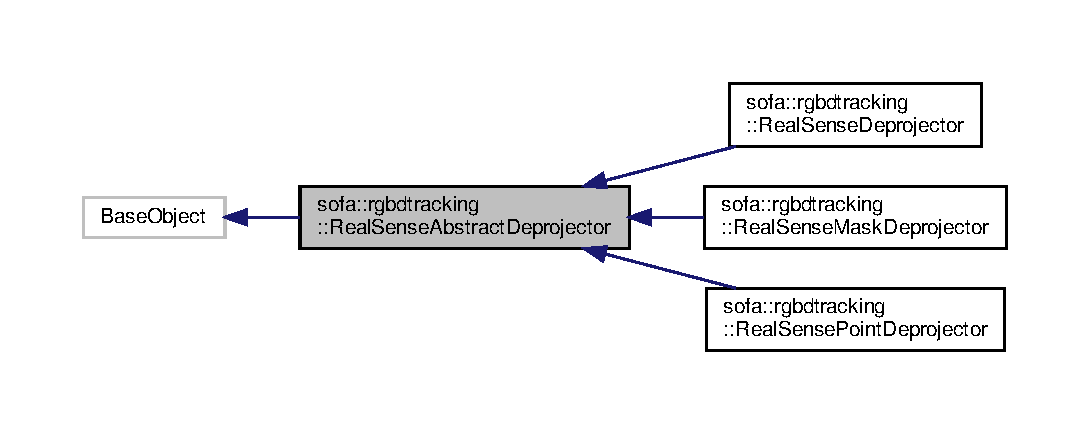
\includegraphics[width=350pt]{classsofa_1_1rgbdtracking_1_1_real_sense_abstract_deprojector__inherit__graph}
\end{center}
\end{figure}


Collaboration diagram for sofa\+:\+:rgbdtracking\+:\+:Real\+Sense\+Abstract\+Deprojector\+:\nopagebreak
\begin{figure}[H]
\begin{center}
\leavevmode
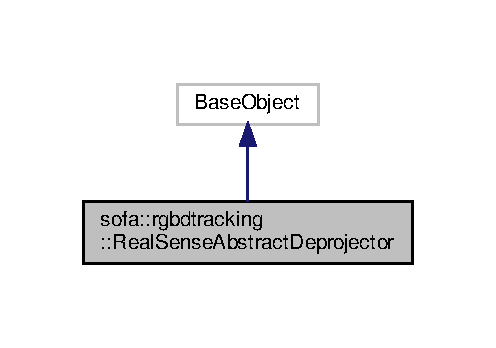
\includegraphics[width=238pt]{classsofa_1_1rgbdtracking_1_1_real_sense_abstract_deprojector__coll__graph}
\end{center}
\end{figure}
\subsection*{Public Types}
\begin{DoxyCompactItemize}
\item 
typedef core\+::objectmodel\+::\+Base\+Object \hyperlink{classsofa_1_1rgbdtracking_1_1_real_sense_abstract_deprojector_a9b4cae154f99cca58b05da9c4b0084ab}{Inherited}
\end{DoxyCompactItemize}
\subsection*{Public Member Functions}
\begin{DoxyCompactItemize}
\item 
\hyperlink{classsofa_1_1rgbdtracking_1_1_real_sense_abstract_deprojector_a595c10a0bf6eb93a562e9cb12dd269b7}{S\+O\+F\+A\+\_\+\+C\+L\+A\+SS} (\hyperlink{classsofa_1_1rgbdtracking_1_1_real_sense_abstract_deprojector}{Real\+Sense\+Abstract\+Deprojector}, core\+::objectmodel\+::\+Base\+Object)
\item 
\hyperlink{classsofa_1_1rgbdtracking_1_1_real_sense_abstract_deprojector_ab427c89296422fbb9184ecf328b9c05d}{Real\+Sense\+Abstract\+Deprojector} ()
\item 
void \hyperlink{classsofa_1_1rgbdtracking_1_1_real_sense_abstract_deprojector_ac809ca0096bb6ec5f003194ecef42533}{init} ()
\item 
void \hyperlink{classsofa_1_1rgbdtracking_1_1_real_sense_abstract_deprojector_a9b933303db901af2174388a524b671a1}{read\+Intrinsics} ()
\begin{DoxyCompactList}\small\item\em read\+Intrinsics reads from a specified file (data \char`\"{}intrinsics\char`\"{}) to rs2\+\_\+intrinsics cam\+\_\+intrinsics \end{DoxyCompactList}\item 
void \hyperlink{classsofa_1_1rgbdtracking_1_1_real_sense_abstract_deprojector_a7b8c549b1df30b374c1431594bcac52b}{deproject\+\_\+image} ()
\begin{DoxyCompactList}\small\item\em deproject\+\_\+image dispatches data processing depending on data (link to realsense cam or not) \end{DoxyCompactList}\item 
void \hyperlink{classsofa_1_1rgbdtracking_1_1_real_sense_abstract_deprojector_ac0889ca4dee6e9980f9f28909d6f3ba6}{deproject\+\_\+image\+\_\+offline} ()
\begin{DoxyCompactList}\small\item\em deproject\+\_\+image\+\_\+offline Load depth/distframe from saved files \end{DoxyCompactList}\item 
void \hyperlink{classsofa_1_1rgbdtracking_1_1_real_sense_abstract_deprojector_a899c0a0245338c2b771138f667d1825c}{deproject\+\_\+image\+\_\+online} ()
\begin{DoxyCompactList}\small\item\em deproject\+\_\+image\+\_\+online get depth/distframe/intrinsics.. from realsense cam \end{DoxyCompactList}\item 
void \hyperlink{classsofa_1_1rgbdtracking_1_1_real_sense_abstract_deprojector_a6e270c7bba84a068595aa361aa3f5f3c}{draw} (const core\+::visual\+::\+Visual\+Params $\ast$vparams)
\item 
void \hyperlink{classsofa_1_1rgbdtracking_1_1_real_sense_abstract_deprojector_ad8bc6a2a7cfe182481496dd4e10e6e42}{push\+\_\+to\+\_\+pointcloud} (helper\+::vector$<$ defaulttype\+::\+Vector3 $>$ \&outpoints, size\+\_\+t i, size\+\_\+t j, int index, \hyperlink{structsofa_1_1rgbdtracking_1_1_real_sense_dist_frame_1_1_real_sense_dist_struct}{Real\+Sense\+Dist\+Frame\+::\+Real\+Sense\+Dist\+Struct} \&diststruct, float dist)
\item 
void \hyperlink{classsofa_1_1rgbdtracking_1_1_real_sense_abstract_deprojector_a8f8c43ae9871e46e75b3ff462af093ca}{make\+Synthetic\+Volume} ()
\item 
pcl\+::\+Point\+X\+YZ \hyperlink{classsofa_1_1rgbdtracking_1_1_real_sense_abstract_deprojector_a39b77c197afd5fe30322103da8c75b74}{scale\+Point} (float $\ast$point3d)
\end{DoxyCompactItemize}
\subsection*{Public Attributes}
\begin{DoxyCompactItemize}
\item 
Data$<$ opencvplugin\+::\+Image\+Data $>$ \hyperlink{classsofa_1_1rgbdtracking_1_1_real_sense_abstract_deprojector_ae7f5594d19b61c9fb590c52a691640e7}{d\+\_\+depth}
\item 
Data$<$ defaulttype\+::\+Vector3 $>$ \hyperlink{classsofa_1_1rgbdtracking_1_1_real_sense_abstract_deprojector_a2f887b81e72511844e1dccc0bb8f9a2c}{d\+\_\+tr\+\_\+offset}
\item 
Data$<$ helper\+::vector$<$ defaulttype\+::\+Vector3 $>$ $>$ \hyperlink{classsofa_1_1rgbdtracking_1_1_real_sense_abstract_deprojector_a3ef009292c2c22613c774b73b327f366}{d\+\_\+output}
\item 
Data$<$ helper\+::vector$<$ defaulttype\+::\+Vector3 $>$ $>$ \hyperlink{classsofa_1_1rgbdtracking_1_1_real_sense_abstract_deprojector_abe1761bdd6106f7ee1b288bf3846fa71}{d\+\_\+synthvolume}
\item 
Data$<$ pointcloud\+::\+Point\+Cloud\+Data $>$ \hyperlink{classsofa_1_1rgbdtracking_1_1_real_sense_abstract_deprojector_a93bfad0013b406e433cf07e342cdc4b5}{d\+\_\+outpcl}
\item 
Data$<$ opencvplugin\+::\+Track\+Bar1 $>$ \hyperlink{classsofa_1_1rgbdtracking_1_1_real_sense_abstract_deprojector_a01e0cd824f7c1e046f9b8a4b0fb5b8ba}{d\+\_\+scale}
\item 
\hyperlink{namespacesofa_1_1rgbdtracking_a00834a9204a667746fef9a402ccbfb55}{Data\+Callback} \hyperlink{classsofa_1_1rgbdtracking_1_1_real_sense_abstract_deprojector_ac692621d9153db98d722796883b1cb88}{c\+\_\+scale}
\item 
Data$<$ \hyperlink{classsofa_1_1rgbdtracking_1_1_real_sense_dist_frame}{Real\+Sense\+Dist\+Frame} $>$ \hyperlink{classsofa_1_1rgbdtracking_1_1_real_sense_abstract_deprojector_a06f9d1a842d19213587304d7e1889b8d}{d\+\_\+distframe}
\item 
Data$<$ std\+::string $>$ \hyperlink{classsofa_1_1rgbdtracking_1_1_real_sense_abstract_deprojector_a8208172bcb64e5ffa7e3ef36182d9fff}{d\+\_\+intrinsics}
\item 
\hyperlink{namespacesofa_1_1rgbdtracking_a00834a9204a667746fef9a402ccbfb55}{Data\+Callback} \hyperlink{classsofa_1_1rgbdtracking_1_1_real_sense_abstract_deprojector_a1194f7c58abfef73ea623a3bd18b09c7}{c\+\_\+intrinsics}
\item 
Data$<$ opencvplugin\+::\+Track\+Bar2 $>$ \hyperlink{classsofa_1_1rgbdtracking_1_1_real_sense_abstract_deprojector_a8c68e247b9ec182e5b014e1d52ed5284}{d\+\_\+minmax}
\item 
Data$<$ bool $>$ \hyperlink{classsofa_1_1rgbdtracking_1_1_real_sense_abstract_deprojector_a57a20129ea423d43053c11764b39640a}{d\+\_\+flip}
\item 
Data$<$ int $>$ \hyperlink{classsofa_1_1rgbdtracking_1_1_real_sense_abstract_deprojector_aa28563fc31f5d63f1df5b32940a2e305}{d\+\_\+downsampler}
\item 
Data$<$ bool $>$ \hyperlink{classsofa_1_1rgbdtracking_1_1_real_sense_abstract_deprojector_afd99828d27af6b6c40cc17dec09fd818}{d\+\_\+drawpcl}
\item 
Data$<$ int $>$ \hyperlink{classsofa_1_1rgbdtracking_1_1_real_sense_abstract_deprojector_ac850857f7f2460b014b5d16545904231}{d\+\_\+densify}
\item 
core\+::objectmodel\+::\+Single\+Link$<$ \hyperlink{classsofa_1_1rgbdtracking_1_1_real_sense_abstract_deprojector}{Real\+Sense\+Abstract\+Deprojector}, \hyperlink{classsofa_1_1rgbdtracking_1_1_real_sense_cam}{Real\+Sense\+Cam}, Base\+Link\+::\+F\+L\+A\+G\+\_\+\+S\+T\+O\+R\+E\+P\+A\+TH$\vert$Base\+Link\+::\+F\+L\+A\+G\+\_\+\+S\+T\+R\+O\+N\+G\+L\+I\+NK $>$ \hyperlink{classsofa_1_1rgbdtracking_1_1_real_sense_abstract_deprojector_aab3f3872a892158eb75c162ceb9dc270}{l\+\_\+rs\+\_\+cam}
\item 
pcl\+::\+Point\+Cloud$<$ pcl\+::\+Point\+X\+YZ $>$\+::Ptr \hyperlink{classsofa_1_1rgbdtracking_1_1_real_sense_abstract_deprojector_a3317c507cc889b1537c708abb50196da}{m\+\_\+pointcloud}
\item 
rs2\+\_\+intrinsics \hyperlink{classsofa_1_1rgbdtracking_1_1_real_sense_abstract_deprojector_abb8025a1f9a471ec9370263b637271f4}{cam\+\_\+intrinsics}
\end{DoxyCompactItemize}


\subsection{Member Typedef Documentation}
\mbox{\Hypertarget{classsofa_1_1rgbdtracking_1_1_real_sense_abstract_deprojector_a9b4cae154f99cca58b05da9c4b0084ab}\label{classsofa_1_1rgbdtracking_1_1_real_sense_abstract_deprojector_a9b4cae154f99cca58b05da9c4b0084ab}} 
\index{sofa\+::rgbdtracking\+::\+Real\+Sense\+Abstract\+Deprojector@{sofa\+::rgbdtracking\+::\+Real\+Sense\+Abstract\+Deprojector}!Inherited@{Inherited}}
\index{Inherited@{Inherited}!sofa\+::rgbdtracking\+::\+Real\+Sense\+Abstract\+Deprojector@{sofa\+::rgbdtracking\+::\+Real\+Sense\+Abstract\+Deprojector}}
\subsubsection{\texorpdfstring{Inherited}{Inherited}}
{\footnotesize\ttfamily typedef core\+::objectmodel\+::\+Base\+Object \hyperlink{classsofa_1_1rgbdtracking_1_1_real_sense_abstract_deprojector_a9b4cae154f99cca58b05da9c4b0084ab}{sofa\+::rgbdtracking\+::\+Real\+Sense\+Abstract\+Deprojector\+::\+Inherited}}



\subsection{Constructor \& Destructor Documentation}
\mbox{\Hypertarget{classsofa_1_1rgbdtracking_1_1_real_sense_abstract_deprojector_ab427c89296422fbb9184ecf328b9c05d}\label{classsofa_1_1rgbdtracking_1_1_real_sense_abstract_deprojector_ab427c89296422fbb9184ecf328b9c05d}} 
\index{sofa\+::rgbdtracking\+::\+Real\+Sense\+Abstract\+Deprojector@{sofa\+::rgbdtracking\+::\+Real\+Sense\+Abstract\+Deprojector}!Real\+Sense\+Abstract\+Deprojector@{Real\+Sense\+Abstract\+Deprojector}}
\index{Real\+Sense\+Abstract\+Deprojector@{Real\+Sense\+Abstract\+Deprojector}!sofa\+::rgbdtracking\+::\+Real\+Sense\+Abstract\+Deprojector@{sofa\+::rgbdtracking\+::\+Real\+Sense\+Abstract\+Deprojector}}
\subsubsection{\texorpdfstring{Real\+Sense\+Abstract\+Deprojector()}{RealSenseAbstractDeprojector()}}
{\footnotesize\ttfamily sofa\+::rgbdtracking\+::\+Real\+Sense\+Abstract\+Deprojector\+::\+Real\+Sense\+Abstract\+Deprojector (\begin{DoxyParamCaption}{ }\end{DoxyParamCaption})\hspace{0.3cm}{\ttfamily [inline]}}



\subsection{Member Function Documentation}
\mbox{\Hypertarget{classsofa_1_1rgbdtracking_1_1_real_sense_abstract_deprojector_a7b8c549b1df30b374c1431594bcac52b}\label{classsofa_1_1rgbdtracking_1_1_real_sense_abstract_deprojector_a7b8c549b1df30b374c1431594bcac52b}} 
\index{sofa\+::rgbdtracking\+::\+Real\+Sense\+Abstract\+Deprojector@{sofa\+::rgbdtracking\+::\+Real\+Sense\+Abstract\+Deprojector}!deproject\+\_\+image@{deproject\+\_\+image}}
\index{deproject\+\_\+image@{deproject\+\_\+image}!sofa\+::rgbdtracking\+::\+Real\+Sense\+Abstract\+Deprojector@{sofa\+::rgbdtracking\+::\+Real\+Sense\+Abstract\+Deprojector}}
\subsubsection{\texorpdfstring{deproject\+\_\+image()}{deproject\_image()}}
{\footnotesize\ttfamily void sofa\+::rgbdtracking\+::\+Real\+Sense\+Abstract\+Deprojector\+::deproject\+\_\+image (\begin{DoxyParamCaption}{ }\end{DoxyParamCaption})\hspace{0.3cm}{\ttfamily [inline]}}



deproject\+\_\+image dispatches data processing depending on data (link to realsense cam or not) 

\mbox{\Hypertarget{classsofa_1_1rgbdtracking_1_1_real_sense_abstract_deprojector_ac0889ca4dee6e9980f9f28909d6f3ba6}\label{classsofa_1_1rgbdtracking_1_1_real_sense_abstract_deprojector_ac0889ca4dee6e9980f9f28909d6f3ba6}} 
\index{sofa\+::rgbdtracking\+::\+Real\+Sense\+Abstract\+Deprojector@{sofa\+::rgbdtracking\+::\+Real\+Sense\+Abstract\+Deprojector}!deproject\+\_\+image\+\_\+offline@{deproject\+\_\+image\+\_\+offline}}
\index{deproject\+\_\+image\+\_\+offline@{deproject\+\_\+image\+\_\+offline}!sofa\+::rgbdtracking\+::\+Real\+Sense\+Abstract\+Deprojector@{sofa\+::rgbdtracking\+::\+Real\+Sense\+Abstract\+Deprojector}}
\subsubsection{\texorpdfstring{deproject\+\_\+image\+\_\+offline()}{deproject\_image\_offline()}}
{\footnotesize\ttfamily void sofa\+::rgbdtracking\+::\+Real\+Sense\+Abstract\+Deprojector\+::deproject\+\_\+image\+\_\+offline (\begin{DoxyParamCaption}{ }\end{DoxyParamCaption})\hspace{0.3cm}{\ttfamily [inline]}}



deproject\+\_\+image\+\_\+offline Load depth/distframe from saved files 

\mbox{\Hypertarget{classsofa_1_1rgbdtracking_1_1_real_sense_abstract_deprojector_a899c0a0245338c2b771138f667d1825c}\label{classsofa_1_1rgbdtracking_1_1_real_sense_abstract_deprojector_a899c0a0245338c2b771138f667d1825c}} 
\index{sofa\+::rgbdtracking\+::\+Real\+Sense\+Abstract\+Deprojector@{sofa\+::rgbdtracking\+::\+Real\+Sense\+Abstract\+Deprojector}!deproject\+\_\+image\+\_\+online@{deproject\+\_\+image\+\_\+online}}
\index{deproject\+\_\+image\+\_\+online@{deproject\+\_\+image\+\_\+online}!sofa\+::rgbdtracking\+::\+Real\+Sense\+Abstract\+Deprojector@{sofa\+::rgbdtracking\+::\+Real\+Sense\+Abstract\+Deprojector}}
\subsubsection{\texorpdfstring{deproject\+\_\+image\+\_\+online()}{deproject\_image\_online()}}
{\footnotesize\ttfamily void sofa\+::rgbdtracking\+::\+Real\+Sense\+Abstract\+Deprojector\+::deproject\+\_\+image\+\_\+online (\begin{DoxyParamCaption}{ }\end{DoxyParamCaption})\hspace{0.3cm}{\ttfamily [inline]}}



deproject\+\_\+image\+\_\+online get depth/distframe/intrinsics.. from realsense cam 

\mbox{\Hypertarget{classsofa_1_1rgbdtracking_1_1_real_sense_abstract_deprojector_a6e270c7bba84a068595aa361aa3f5f3c}\label{classsofa_1_1rgbdtracking_1_1_real_sense_abstract_deprojector_a6e270c7bba84a068595aa361aa3f5f3c}} 
\index{sofa\+::rgbdtracking\+::\+Real\+Sense\+Abstract\+Deprojector@{sofa\+::rgbdtracking\+::\+Real\+Sense\+Abstract\+Deprojector}!draw@{draw}}
\index{draw@{draw}!sofa\+::rgbdtracking\+::\+Real\+Sense\+Abstract\+Deprojector@{sofa\+::rgbdtracking\+::\+Real\+Sense\+Abstract\+Deprojector}}
\subsubsection{\texorpdfstring{draw()}{draw()}}
{\footnotesize\ttfamily void sofa\+::rgbdtracking\+::\+Real\+Sense\+Abstract\+Deprojector\+::draw (\begin{DoxyParamCaption}\item[{const core\+::visual\+::\+Visual\+Params $\ast$}]{vparams }\end{DoxyParamCaption})\hspace{0.3cm}{\ttfamily [inline]}}

\mbox{\Hypertarget{classsofa_1_1rgbdtracking_1_1_real_sense_abstract_deprojector_ac809ca0096bb6ec5f003194ecef42533}\label{classsofa_1_1rgbdtracking_1_1_real_sense_abstract_deprojector_ac809ca0096bb6ec5f003194ecef42533}} 
\index{sofa\+::rgbdtracking\+::\+Real\+Sense\+Abstract\+Deprojector@{sofa\+::rgbdtracking\+::\+Real\+Sense\+Abstract\+Deprojector}!init@{init}}
\index{init@{init}!sofa\+::rgbdtracking\+::\+Real\+Sense\+Abstract\+Deprojector@{sofa\+::rgbdtracking\+::\+Real\+Sense\+Abstract\+Deprojector}}
\subsubsection{\texorpdfstring{init()}{init()}}
{\footnotesize\ttfamily void sofa\+::rgbdtracking\+::\+Real\+Sense\+Abstract\+Deprojector\+::init (\begin{DoxyParamCaption}{ }\end{DoxyParamCaption})\hspace{0.3cm}{\ttfamily [inline]}}

\mbox{\Hypertarget{classsofa_1_1rgbdtracking_1_1_real_sense_abstract_deprojector_a8f8c43ae9871e46e75b3ff462af093ca}\label{classsofa_1_1rgbdtracking_1_1_real_sense_abstract_deprojector_a8f8c43ae9871e46e75b3ff462af093ca}} 
\index{sofa\+::rgbdtracking\+::\+Real\+Sense\+Abstract\+Deprojector@{sofa\+::rgbdtracking\+::\+Real\+Sense\+Abstract\+Deprojector}!make\+Synthetic\+Volume@{make\+Synthetic\+Volume}}
\index{make\+Synthetic\+Volume@{make\+Synthetic\+Volume}!sofa\+::rgbdtracking\+::\+Real\+Sense\+Abstract\+Deprojector@{sofa\+::rgbdtracking\+::\+Real\+Sense\+Abstract\+Deprojector}}
\subsubsection{\texorpdfstring{make\+Synthetic\+Volume()}{makeSyntheticVolume()}}
{\footnotesize\ttfamily void sofa\+::rgbdtracking\+::\+Real\+Sense\+Abstract\+Deprojector\+::make\+Synthetic\+Volume (\begin{DoxyParamCaption}{ }\end{DoxyParamCaption})\hspace{0.3cm}{\ttfamily [inline]}}

\mbox{\Hypertarget{classsofa_1_1rgbdtracking_1_1_real_sense_abstract_deprojector_ad8bc6a2a7cfe182481496dd4e10e6e42}\label{classsofa_1_1rgbdtracking_1_1_real_sense_abstract_deprojector_ad8bc6a2a7cfe182481496dd4e10e6e42}} 
\index{sofa\+::rgbdtracking\+::\+Real\+Sense\+Abstract\+Deprojector@{sofa\+::rgbdtracking\+::\+Real\+Sense\+Abstract\+Deprojector}!push\+\_\+to\+\_\+pointcloud@{push\+\_\+to\+\_\+pointcloud}}
\index{push\+\_\+to\+\_\+pointcloud@{push\+\_\+to\+\_\+pointcloud}!sofa\+::rgbdtracking\+::\+Real\+Sense\+Abstract\+Deprojector@{sofa\+::rgbdtracking\+::\+Real\+Sense\+Abstract\+Deprojector}}
\subsubsection{\texorpdfstring{push\+\_\+to\+\_\+pointcloud()}{push\_to\_pointcloud()}}
{\footnotesize\ttfamily void sofa\+::rgbdtracking\+::\+Real\+Sense\+Abstract\+Deprojector\+::push\+\_\+to\+\_\+pointcloud (\begin{DoxyParamCaption}\item[{helper\+::vector$<$ defaulttype\+::\+Vector3 $>$ \&}]{outpoints,  }\item[{size\+\_\+t}]{i,  }\item[{size\+\_\+t}]{j,  }\item[{int}]{index,  }\item[{\hyperlink{structsofa_1_1rgbdtracking_1_1_real_sense_dist_frame_1_1_real_sense_dist_struct}{Real\+Sense\+Dist\+Frame\+::\+Real\+Sense\+Dist\+Struct} \&}]{diststruct,  }\item[{float}]{dist }\end{DoxyParamCaption})\hspace{0.3cm}{\ttfamily [inline]}}

\mbox{\Hypertarget{classsofa_1_1rgbdtracking_1_1_real_sense_abstract_deprojector_a9b933303db901af2174388a524b671a1}\label{classsofa_1_1rgbdtracking_1_1_real_sense_abstract_deprojector_a9b933303db901af2174388a524b671a1}} 
\index{sofa\+::rgbdtracking\+::\+Real\+Sense\+Abstract\+Deprojector@{sofa\+::rgbdtracking\+::\+Real\+Sense\+Abstract\+Deprojector}!read\+Intrinsics@{read\+Intrinsics}}
\index{read\+Intrinsics@{read\+Intrinsics}!sofa\+::rgbdtracking\+::\+Real\+Sense\+Abstract\+Deprojector@{sofa\+::rgbdtracking\+::\+Real\+Sense\+Abstract\+Deprojector}}
\subsubsection{\texorpdfstring{read\+Intrinsics()}{readIntrinsics()}}
{\footnotesize\ttfamily void sofa\+::rgbdtracking\+::\+Real\+Sense\+Abstract\+Deprojector\+::read\+Intrinsics (\begin{DoxyParamCaption}{ }\end{DoxyParamCaption})\hspace{0.3cm}{\ttfamily [inline]}}



read\+Intrinsics reads from a specified file (data \char`\"{}intrinsics\char`\"{}) to rs2\+\_\+intrinsics cam\+\_\+intrinsics 

\mbox{\Hypertarget{classsofa_1_1rgbdtracking_1_1_real_sense_abstract_deprojector_a39b77c197afd5fe30322103da8c75b74}\label{classsofa_1_1rgbdtracking_1_1_real_sense_abstract_deprojector_a39b77c197afd5fe30322103da8c75b74}} 
\index{sofa\+::rgbdtracking\+::\+Real\+Sense\+Abstract\+Deprojector@{sofa\+::rgbdtracking\+::\+Real\+Sense\+Abstract\+Deprojector}!scale\+Point@{scale\+Point}}
\index{scale\+Point@{scale\+Point}!sofa\+::rgbdtracking\+::\+Real\+Sense\+Abstract\+Deprojector@{sofa\+::rgbdtracking\+::\+Real\+Sense\+Abstract\+Deprojector}}
\subsubsection{\texorpdfstring{scale\+Point()}{scalePoint()}}
{\footnotesize\ttfamily pcl\+::\+Point\+X\+YZ sofa\+::rgbdtracking\+::\+Real\+Sense\+Abstract\+Deprojector\+::scale\+Point (\begin{DoxyParamCaption}\item[{float $\ast$}]{point3d }\end{DoxyParamCaption})\hspace{0.3cm}{\ttfamily [inline]}}

\mbox{\Hypertarget{classsofa_1_1rgbdtracking_1_1_real_sense_abstract_deprojector_a595c10a0bf6eb93a562e9cb12dd269b7}\label{classsofa_1_1rgbdtracking_1_1_real_sense_abstract_deprojector_a595c10a0bf6eb93a562e9cb12dd269b7}} 
\index{sofa\+::rgbdtracking\+::\+Real\+Sense\+Abstract\+Deprojector@{sofa\+::rgbdtracking\+::\+Real\+Sense\+Abstract\+Deprojector}!S\+O\+F\+A\+\_\+\+C\+L\+A\+SS@{S\+O\+F\+A\+\_\+\+C\+L\+A\+SS}}
\index{S\+O\+F\+A\+\_\+\+C\+L\+A\+SS@{S\+O\+F\+A\+\_\+\+C\+L\+A\+SS}!sofa\+::rgbdtracking\+::\+Real\+Sense\+Abstract\+Deprojector@{sofa\+::rgbdtracking\+::\+Real\+Sense\+Abstract\+Deprojector}}
\subsubsection{\texorpdfstring{S\+O\+F\+A\+\_\+\+C\+L\+A\+S\+S()}{SOFA\_CLASS()}}
{\footnotesize\ttfamily sofa\+::rgbdtracking\+::\+Real\+Sense\+Abstract\+Deprojector\+::\+S\+O\+F\+A\+\_\+\+C\+L\+A\+SS (\begin{DoxyParamCaption}\item[{\hyperlink{classsofa_1_1rgbdtracking_1_1_real_sense_abstract_deprojector}{Real\+Sense\+Abstract\+Deprojector}}]{,  }\item[{core\+::objectmodel\+::\+Base\+Object}]{ }\end{DoxyParamCaption})}



\subsection{Member Data Documentation}
\mbox{\Hypertarget{classsofa_1_1rgbdtracking_1_1_real_sense_abstract_deprojector_a1194f7c58abfef73ea623a3bd18b09c7}\label{classsofa_1_1rgbdtracking_1_1_real_sense_abstract_deprojector_a1194f7c58abfef73ea623a3bd18b09c7}} 
\index{sofa\+::rgbdtracking\+::\+Real\+Sense\+Abstract\+Deprojector@{sofa\+::rgbdtracking\+::\+Real\+Sense\+Abstract\+Deprojector}!c\+\_\+intrinsics@{c\+\_\+intrinsics}}
\index{c\+\_\+intrinsics@{c\+\_\+intrinsics}!sofa\+::rgbdtracking\+::\+Real\+Sense\+Abstract\+Deprojector@{sofa\+::rgbdtracking\+::\+Real\+Sense\+Abstract\+Deprojector}}
\subsubsection{\texorpdfstring{c\+\_\+intrinsics}{c\_intrinsics}}
{\footnotesize\ttfamily \hyperlink{namespacesofa_1_1rgbdtracking_a00834a9204a667746fef9a402ccbfb55}{Data\+Callback} sofa\+::rgbdtracking\+::\+Real\+Sense\+Abstract\+Deprojector\+::c\+\_\+intrinsics}

\mbox{\Hypertarget{classsofa_1_1rgbdtracking_1_1_real_sense_abstract_deprojector_ac692621d9153db98d722796883b1cb88}\label{classsofa_1_1rgbdtracking_1_1_real_sense_abstract_deprojector_ac692621d9153db98d722796883b1cb88}} 
\index{sofa\+::rgbdtracking\+::\+Real\+Sense\+Abstract\+Deprojector@{sofa\+::rgbdtracking\+::\+Real\+Sense\+Abstract\+Deprojector}!c\+\_\+scale@{c\+\_\+scale}}
\index{c\+\_\+scale@{c\+\_\+scale}!sofa\+::rgbdtracking\+::\+Real\+Sense\+Abstract\+Deprojector@{sofa\+::rgbdtracking\+::\+Real\+Sense\+Abstract\+Deprojector}}
\subsubsection{\texorpdfstring{c\+\_\+scale}{c\_scale}}
{\footnotesize\ttfamily \hyperlink{namespacesofa_1_1rgbdtracking_a00834a9204a667746fef9a402ccbfb55}{Data\+Callback} sofa\+::rgbdtracking\+::\+Real\+Sense\+Abstract\+Deprojector\+::c\+\_\+scale}

\mbox{\Hypertarget{classsofa_1_1rgbdtracking_1_1_real_sense_abstract_deprojector_abb8025a1f9a471ec9370263b637271f4}\label{classsofa_1_1rgbdtracking_1_1_real_sense_abstract_deprojector_abb8025a1f9a471ec9370263b637271f4}} 
\index{sofa\+::rgbdtracking\+::\+Real\+Sense\+Abstract\+Deprojector@{sofa\+::rgbdtracking\+::\+Real\+Sense\+Abstract\+Deprojector}!cam\+\_\+intrinsics@{cam\+\_\+intrinsics}}
\index{cam\+\_\+intrinsics@{cam\+\_\+intrinsics}!sofa\+::rgbdtracking\+::\+Real\+Sense\+Abstract\+Deprojector@{sofa\+::rgbdtracking\+::\+Real\+Sense\+Abstract\+Deprojector}}
\subsubsection{\texorpdfstring{cam\+\_\+intrinsics}{cam\_intrinsics}}
{\footnotesize\ttfamily rs2\+\_\+intrinsics sofa\+::rgbdtracking\+::\+Real\+Sense\+Abstract\+Deprojector\+::cam\+\_\+intrinsics}

\mbox{\Hypertarget{classsofa_1_1rgbdtracking_1_1_real_sense_abstract_deprojector_ac850857f7f2460b014b5d16545904231}\label{classsofa_1_1rgbdtracking_1_1_real_sense_abstract_deprojector_ac850857f7f2460b014b5d16545904231}} 
\index{sofa\+::rgbdtracking\+::\+Real\+Sense\+Abstract\+Deprojector@{sofa\+::rgbdtracking\+::\+Real\+Sense\+Abstract\+Deprojector}!d\+\_\+densify@{d\+\_\+densify}}
\index{d\+\_\+densify@{d\+\_\+densify}!sofa\+::rgbdtracking\+::\+Real\+Sense\+Abstract\+Deprojector@{sofa\+::rgbdtracking\+::\+Real\+Sense\+Abstract\+Deprojector}}
\subsubsection{\texorpdfstring{d\+\_\+densify}{d\_densify}}
{\footnotesize\ttfamily Data$<$int$>$ sofa\+::rgbdtracking\+::\+Real\+Sense\+Abstract\+Deprojector\+::d\+\_\+densify}

\mbox{\Hypertarget{classsofa_1_1rgbdtracking_1_1_real_sense_abstract_deprojector_ae7f5594d19b61c9fb590c52a691640e7}\label{classsofa_1_1rgbdtracking_1_1_real_sense_abstract_deprojector_ae7f5594d19b61c9fb590c52a691640e7}} 
\index{sofa\+::rgbdtracking\+::\+Real\+Sense\+Abstract\+Deprojector@{sofa\+::rgbdtracking\+::\+Real\+Sense\+Abstract\+Deprojector}!d\+\_\+depth@{d\+\_\+depth}}
\index{d\+\_\+depth@{d\+\_\+depth}!sofa\+::rgbdtracking\+::\+Real\+Sense\+Abstract\+Deprojector@{sofa\+::rgbdtracking\+::\+Real\+Sense\+Abstract\+Deprojector}}
\subsubsection{\texorpdfstring{d\+\_\+depth}{d\_depth}}
{\footnotesize\ttfamily Data$<$opencvplugin\+::\+Image\+Data$>$ sofa\+::rgbdtracking\+::\+Real\+Sense\+Abstract\+Deprojector\+::d\+\_\+depth}

\mbox{\Hypertarget{classsofa_1_1rgbdtracking_1_1_real_sense_abstract_deprojector_a06f9d1a842d19213587304d7e1889b8d}\label{classsofa_1_1rgbdtracking_1_1_real_sense_abstract_deprojector_a06f9d1a842d19213587304d7e1889b8d}} 
\index{sofa\+::rgbdtracking\+::\+Real\+Sense\+Abstract\+Deprojector@{sofa\+::rgbdtracking\+::\+Real\+Sense\+Abstract\+Deprojector}!d\+\_\+distframe@{d\+\_\+distframe}}
\index{d\+\_\+distframe@{d\+\_\+distframe}!sofa\+::rgbdtracking\+::\+Real\+Sense\+Abstract\+Deprojector@{sofa\+::rgbdtracking\+::\+Real\+Sense\+Abstract\+Deprojector}}
\subsubsection{\texorpdfstring{d\+\_\+distframe}{d\_distframe}}
{\footnotesize\ttfamily Data$<$\hyperlink{classsofa_1_1rgbdtracking_1_1_real_sense_dist_frame}{Real\+Sense\+Dist\+Frame}$>$ sofa\+::rgbdtracking\+::\+Real\+Sense\+Abstract\+Deprojector\+::d\+\_\+distframe}

\mbox{\Hypertarget{classsofa_1_1rgbdtracking_1_1_real_sense_abstract_deprojector_aa28563fc31f5d63f1df5b32940a2e305}\label{classsofa_1_1rgbdtracking_1_1_real_sense_abstract_deprojector_aa28563fc31f5d63f1df5b32940a2e305}} 
\index{sofa\+::rgbdtracking\+::\+Real\+Sense\+Abstract\+Deprojector@{sofa\+::rgbdtracking\+::\+Real\+Sense\+Abstract\+Deprojector}!d\+\_\+downsampler@{d\+\_\+downsampler}}
\index{d\+\_\+downsampler@{d\+\_\+downsampler}!sofa\+::rgbdtracking\+::\+Real\+Sense\+Abstract\+Deprojector@{sofa\+::rgbdtracking\+::\+Real\+Sense\+Abstract\+Deprojector}}
\subsubsection{\texorpdfstring{d\+\_\+downsampler}{d\_downsampler}}
{\footnotesize\ttfamily Data$<$int$>$ sofa\+::rgbdtracking\+::\+Real\+Sense\+Abstract\+Deprojector\+::d\+\_\+downsampler}

\mbox{\Hypertarget{classsofa_1_1rgbdtracking_1_1_real_sense_abstract_deprojector_afd99828d27af6b6c40cc17dec09fd818}\label{classsofa_1_1rgbdtracking_1_1_real_sense_abstract_deprojector_afd99828d27af6b6c40cc17dec09fd818}} 
\index{sofa\+::rgbdtracking\+::\+Real\+Sense\+Abstract\+Deprojector@{sofa\+::rgbdtracking\+::\+Real\+Sense\+Abstract\+Deprojector}!d\+\_\+drawpcl@{d\+\_\+drawpcl}}
\index{d\+\_\+drawpcl@{d\+\_\+drawpcl}!sofa\+::rgbdtracking\+::\+Real\+Sense\+Abstract\+Deprojector@{sofa\+::rgbdtracking\+::\+Real\+Sense\+Abstract\+Deprojector}}
\subsubsection{\texorpdfstring{d\+\_\+drawpcl}{d\_drawpcl}}
{\footnotesize\ttfamily Data$<$bool$>$ sofa\+::rgbdtracking\+::\+Real\+Sense\+Abstract\+Deprojector\+::d\+\_\+drawpcl}

\mbox{\Hypertarget{classsofa_1_1rgbdtracking_1_1_real_sense_abstract_deprojector_a57a20129ea423d43053c11764b39640a}\label{classsofa_1_1rgbdtracking_1_1_real_sense_abstract_deprojector_a57a20129ea423d43053c11764b39640a}} 
\index{sofa\+::rgbdtracking\+::\+Real\+Sense\+Abstract\+Deprojector@{sofa\+::rgbdtracking\+::\+Real\+Sense\+Abstract\+Deprojector}!d\+\_\+flip@{d\+\_\+flip}}
\index{d\+\_\+flip@{d\+\_\+flip}!sofa\+::rgbdtracking\+::\+Real\+Sense\+Abstract\+Deprojector@{sofa\+::rgbdtracking\+::\+Real\+Sense\+Abstract\+Deprojector}}
\subsubsection{\texorpdfstring{d\+\_\+flip}{d\_flip}}
{\footnotesize\ttfamily Data$<$bool$>$ sofa\+::rgbdtracking\+::\+Real\+Sense\+Abstract\+Deprojector\+::d\+\_\+flip}

\mbox{\Hypertarget{classsofa_1_1rgbdtracking_1_1_real_sense_abstract_deprojector_a8208172bcb64e5ffa7e3ef36182d9fff}\label{classsofa_1_1rgbdtracking_1_1_real_sense_abstract_deprojector_a8208172bcb64e5ffa7e3ef36182d9fff}} 
\index{sofa\+::rgbdtracking\+::\+Real\+Sense\+Abstract\+Deprojector@{sofa\+::rgbdtracking\+::\+Real\+Sense\+Abstract\+Deprojector}!d\+\_\+intrinsics@{d\+\_\+intrinsics}}
\index{d\+\_\+intrinsics@{d\+\_\+intrinsics}!sofa\+::rgbdtracking\+::\+Real\+Sense\+Abstract\+Deprojector@{sofa\+::rgbdtracking\+::\+Real\+Sense\+Abstract\+Deprojector}}
\subsubsection{\texorpdfstring{d\+\_\+intrinsics}{d\_intrinsics}}
{\footnotesize\ttfamily Data$<$std\+::string$>$ sofa\+::rgbdtracking\+::\+Real\+Sense\+Abstract\+Deprojector\+::d\+\_\+intrinsics}

\mbox{\Hypertarget{classsofa_1_1rgbdtracking_1_1_real_sense_abstract_deprojector_a8c68e247b9ec182e5b014e1d52ed5284}\label{classsofa_1_1rgbdtracking_1_1_real_sense_abstract_deprojector_a8c68e247b9ec182e5b014e1d52ed5284}} 
\index{sofa\+::rgbdtracking\+::\+Real\+Sense\+Abstract\+Deprojector@{sofa\+::rgbdtracking\+::\+Real\+Sense\+Abstract\+Deprojector}!d\+\_\+minmax@{d\+\_\+minmax}}
\index{d\+\_\+minmax@{d\+\_\+minmax}!sofa\+::rgbdtracking\+::\+Real\+Sense\+Abstract\+Deprojector@{sofa\+::rgbdtracking\+::\+Real\+Sense\+Abstract\+Deprojector}}
\subsubsection{\texorpdfstring{d\+\_\+minmax}{d\_minmax}}
{\footnotesize\ttfamily Data$<$opencvplugin\+::\+Track\+Bar2$>$ sofa\+::rgbdtracking\+::\+Real\+Sense\+Abstract\+Deprojector\+::d\+\_\+minmax}

\mbox{\Hypertarget{classsofa_1_1rgbdtracking_1_1_real_sense_abstract_deprojector_a93bfad0013b406e433cf07e342cdc4b5}\label{classsofa_1_1rgbdtracking_1_1_real_sense_abstract_deprojector_a93bfad0013b406e433cf07e342cdc4b5}} 
\index{sofa\+::rgbdtracking\+::\+Real\+Sense\+Abstract\+Deprojector@{sofa\+::rgbdtracking\+::\+Real\+Sense\+Abstract\+Deprojector}!d\+\_\+outpcl@{d\+\_\+outpcl}}
\index{d\+\_\+outpcl@{d\+\_\+outpcl}!sofa\+::rgbdtracking\+::\+Real\+Sense\+Abstract\+Deprojector@{sofa\+::rgbdtracking\+::\+Real\+Sense\+Abstract\+Deprojector}}
\subsubsection{\texorpdfstring{d\+\_\+outpcl}{d\_outpcl}}
{\footnotesize\ttfamily Data$<$pointcloud\+::\+Point\+Cloud\+Data$>$ sofa\+::rgbdtracking\+::\+Real\+Sense\+Abstract\+Deprojector\+::d\+\_\+outpcl}

\mbox{\Hypertarget{classsofa_1_1rgbdtracking_1_1_real_sense_abstract_deprojector_a3ef009292c2c22613c774b73b327f366}\label{classsofa_1_1rgbdtracking_1_1_real_sense_abstract_deprojector_a3ef009292c2c22613c774b73b327f366}} 
\index{sofa\+::rgbdtracking\+::\+Real\+Sense\+Abstract\+Deprojector@{sofa\+::rgbdtracking\+::\+Real\+Sense\+Abstract\+Deprojector}!d\+\_\+output@{d\+\_\+output}}
\index{d\+\_\+output@{d\+\_\+output}!sofa\+::rgbdtracking\+::\+Real\+Sense\+Abstract\+Deprojector@{sofa\+::rgbdtracking\+::\+Real\+Sense\+Abstract\+Deprojector}}
\subsubsection{\texorpdfstring{d\+\_\+output}{d\_output}}
{\footnotesize\ttfamily Data$<$helper\+::vector$<$defaulttype\+::\+Vector3$>$ $>$ sofa\+::rgbdtracking\+::\+Real\+Sense\+Abstract\+Deprojector\+::d\+\_\+output}

\mbox{\Hypertarget{classsofa_1_1rgbdtracking_1_1_real_sense_abstract_deprojector_a01e0cd824f7c1e046f9b8a4b0fb5b8ba}\label{classsofa_1_1rgbdtracking_1_1_real_sense_abstract_deprojector_a01e0cd824f7c1e046f9b8a4b0fb5b8ba}} 
\index{sofa\+::rgbdtracking\+::\+Real\+Sense\+Abstract\+Deprojector@{sofa\+::rgbdtracking\+::\+Real\+Sense\+Abstract\+Deprojector}!d\+\_\+scale@{d\+\_\+scale}}
\index{d\+\_\+scale@{d\+\_\+scale}!sofa\+::rgbdtracking\+::\+Real\+Sense\+Abstract\+Deprojector@{sofa\+::rgbdtracking\+::\+Real\+Sense\+Abstract\+Deprojector}}
\subsubsection{\texorpdfstring{d\+\_\+scale}{d\_scale}}
{\footnotesize\ttfamily Data$<$opencvplugin\+::\+Track\+Bar1$>$ sofa\+::rgbdtracking\+::\+Real\+Sense\+Abstract\+Deprojector\+::d\+\_\+scale}

\mbox{\Hypertarget{classsofa_1_1rgbdtracking_1_1_real_sense_abstract_deprojector_abe1761bdd6106f7ee1b288bf3846fa71}\label{classsofa_1_1rgbdtracking_1_1_real_sense_abstract_deprojector_abe1761bdd6106f7ee1b288bf3846fa71}} 
\index{sofa\+::rgbdtracking\+::\+Real\+Sense\+Abstract\+Deprojector@{sofa\+::rgbdtracking\+::\+Real\+Sense\+Abstract\+Deprojector}!d\+\_\+synthvolume@{d\+\_\+synthvolume}}
\index{d\+\_\+synthvolume@{d\+\_\+synthvolume}!sofa\+::rgbdtracking\+::\+Real\+Sense\+Abstract\+Deprojector@{sofa\+::rgbdtracking\+::\+Real\+Sense\+Abstract\+Deprojector}}
\subsubsection{\texorpdfstring{d\+\_\+synthvolume}{d\_synthvolume}}
{\footnotesize\ttfamily Data$<$helper\+::vector$<$defaulttype\+::\+Vector3$>$ $>$ sofa\+::rgbdtracking\+::\+Real\+Sense\+Abstract\+Deprojector\+::d\+\_\+synthvolume}

\mbox{\Hypertarget{classsofa_1_1rgbdtracking_1_1_real_sense_abstract_deprojector_a2f887b81e72511844e1dccc0bb8f9a2c}\label{classsofa_1_1rgbdtracking_1_1_real_sense_abstract_deprojector_a2f887b81e72511844e1dccc0bb8f9a2c}} 
\index{sofa\+::rgbdtracking\+::\+Real\+Sense\+Abstract\+Deprojector@{sofa\+::rgbdtracking\+::\+Real\+Sense\+Abstract\+Deprojector}!d\+\_\+tr\+\_\+offset@{d\+\_\+tr\+\_\+offset}}
\index{d\+\_\+tr\+\_\+offset@{d\+\_\+tr\+\_\+offset}!sofa\+::rgbdtracking\+::\+Real\+Sense\+Abstract\+Deprojector@{sofa\+::rgbdtracking\+::\+Real\+Sense\+Abstract\+Deprojector}}
\subsubsection{\texorpdfstring{d\+\_\+tr\+\_\+offset}{d\_tr\_offset}}
{\footnotesize\ttfamily Data$<$defaulttype\+::\+Vector3$>$ sofa\+::rgbdtracking\+::\+Real\+Sense\+Abstract\+Deprojector\+::d\+\_\+tr\+\_\+offset}

\mbox{\Hypertarget{classsofa_1_1rgbdtracking_1_1_real_sense_abstract_deprojector_aab3f3872a892158eb75c162ceb9dc270}\label{classsofa_1_1rgbdtracking_1_1_real_sense_abstract_deprojector_aab3f3872a892158eb75c162ceb9dc270}} 
\index{sofa\+::rgbdtracking\+::\+Real\+Sense\+Abstract\+Deprojector@{sofa\+::rgbdtracking\+::\+Real\+Sense\+Abstract\+Deprojector}!l\+\_\+rs\+\_\+cam@{l\+\_\+rs\+\_\+cam}}
\index{l\+\_\+rs\+\_\+cam@{l\+\_\+rs\+\_\+cam}!sofa\+::rgbdtracking\+::\+Real\+Sense\+Abstract\+Deprojector@{sofa\+::rgbdtracking\+::\+Real\+Sense\+Abstract\+Deprojector}}
\subsubsection{\texorpdfstring{l\+\_\+rs\+\_\+cam}{l\_rs\_cam}}
{\footnotesize\ttfamily core\+::objectmodel\+::\+Single\+Link$<$ \hyperlink{classsofa_1_1rgbdtracking_1_1_real_sense_abstract_deprojector}{Real\+Sense\+Abstract\+Deprojector}, \hyperlink{classsofa_1_1rgbdtracking_1_1_real_sense_cam}{Real\+Sense\+Cam}, Base\+Link\+::\+F\+L\+A\+G\+\_\+\+S\+T\+O\+R\+E\+P\+A\+TH$\vert$Base\+Link\+::\+F\+L\+A\+G\+\_\+\+S\+T\+R\+O\+N\+G\+L\+I\+NK $>$ sofa\+::rgbdtracking\+::\+Real\+Sense\+Abstract\+Deprojector\+::l\+\_\+rs\+\_\+cam}

\mbox{\Hypertarget{classsofa_1_1rgbdtracking_1_1_real_sense_abstract_deprojector_a3317c507cc889b1537c708abb50196da}\label{classsofa_1_1rgbdtracking_1_1_real_sense_abstract_deprojector_a3317c507cc889b1537c708abb50196da}} 
\index{sofa\+::rgbdtracking\+::\+Real\+Sense\+Abstract\+Deprojector@{sofa\+::rgbdtracking\+::\+Real\+Sense\+Abstract\+Deprojector}!m\+\_\+pointcloud@{m\+\_\+pointcloud}}
\index{m\+\_\+pointcloud@{m\+\_\+pointcloud}!sofa\+::rgbdtracking\+::\+Real\+Sense\+Abstract\+Deprojector@{sofa\+::rgbdtracking\+::\+Real\+Sense\+Abstract\+Deprojector}}
\subsubsection{\texorpdfstring{m\+\_\+pointcloud}{m\_pointcloud}}
{\footnotesize\ttfamily pcl\+::\+Point\+Cloud$<$pcl\+::\+Point\+X\+YZ$>$\+::Ptr sofa\+::rgbdtracking\+::\+Real\+Sense\+Abstract\+Deprojector\+::m\+\_\+pointcloud}



The documentation for this class was generated from the following file\+:\begin{DoxyCompactItemize}
\item 
src/sofa/realsenseplugin/projector/\hyperlink{_real_sense_abstract_projector_8h}{Real\+Sense\+Abstract\+Projector.\+h}\end{DoxyCompactItemize}

\hypertarget{classsofa_1_1rgbdtracking_1_1_real_sense_calibrator}{}\section{sofa\+:\+:rgbdtracking\+:\+:Real\+Sense\+Calibrator Class Reference}
\label{classsofa_1_1rgbdtracking_1_1_real_sense_calibrator}\index{sofa\+::rgbdtracking\+::\+Real\+Sense\+Calibrator@{sofa\+::rgbdtracking\+::\+Real\+Sense\+Calibrator}}


{\ttfamily \#include $<$Real\+Sense\+Calibrator.\+h$>$}



Inheritance diagram for sofa\+:\+:rgbdtracking\+:\+:Real\+Sense\+Calibrator\+:\nopagebreak
\begin{figure}[H]
\begin{center}
\leavevmode
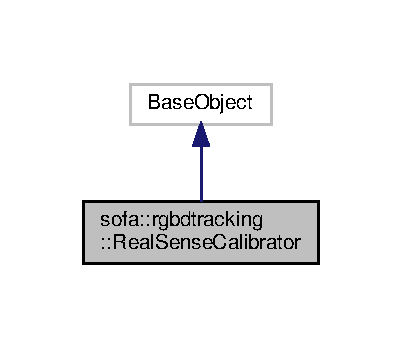
\includegraphics[width=193pt]{classsofa_1_1rgbdtracking_1_1_real_sense_calibrator__inherit__graph}
\end{center}
\end{figure}


Collaboration diagram for sofa\+:\+:rgbdtracking\+:\+:Real\+Sense\+Calibrator\+:\nopagebreak
\begin{figure}[H]
\begin{center}
\leavevmode
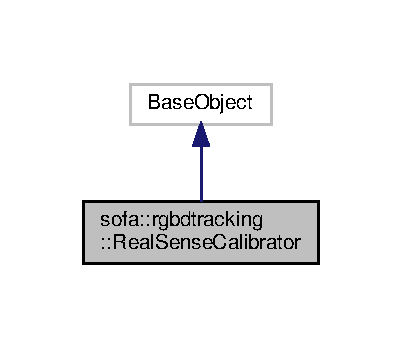
\includegraphics[width=193pt]{classsofa_1_1rgbdtracking_1_1_real_sense_calibrator__coll__graph}
\end{center}
\end{figure}
\subsection*{Public Types}
\begin{DoxyCompactItemize}
\item 
typedef core\+::objectmodel\+::\+Base\+Object \hyperlink{classsofa_1_1rgbdtracking_1_1_real_sense_calibrator_af5eef0eeea5daa52e920b9d29e5575dc}{Inherited}
\end{DoxyCompactItemize}
\subsection*{Public Member Functions}
\begin{DoxyCompactItemize}
\item 
\hyperlink{classsofa_1_1rgbdtracking_1_1_real_sense_calibrator_a65aec8ab1fa6f8bda1ed0b496d818522}{S\+O\+F\+A\+\_\+\+C\+L\+A\+SS} (\hyperlink{classsofa_1_1rgbdtracking_1_1_real_sense_calibrator}{Real\+Sense\+Calibrator}, \hyperlink{classsofa_1_1rgbdtracking_1_1_real_sense_calibrator_af5eef0eeea5daa52e920b9d29e5575dc}{Inherited})
\item 
\hyperlink{classsofa_1_1rgbdtracking_1_1_real_sense_calibrator_a4f171363d7cde684d2f84db2dcf0efe7}{Real\+Sense\+Calibrator} ()
\end{DoxyCompactItemize}


\subsection{Member Typedef Documentation}
\mbox{\Hypertarget{classsofa_1_1rgbdtracking_1_1_real_sense_calibrator_af5eef0eeea5daa52e920b9d29e5575dc}\label{classsofa_1_1rgbdtracking_1_1_real_sense_calibrator_af5eef0eeea5daa52e920b9d29e5575dc}} 
\index{sofa\+::rgbdtracking\+::\+Real\+Sense\+Calibrator@{sofa\+::rgbdtracking\+::\+Real\+Sense\+Calibrator}!Inherited@{Inherited}}
\index{Inherited@{Inherited}!sofa\+::rgbdtracking\+::\+Real\+Sense\+Calibrator@{sofa\+::rgbdtracking\+::\+Real\+Sense\+Calibrator}}
\subsubsection{\texorpdfstring{Inherited}{Inherited}}
{\footnotesize\ttfamily typedef core\+::objectmodel\+::\+Base\+Object \hyperlink{classsofa_1_1rgbdtracking_1_1_real_sense_calibrator_af5eef0eeea5daa52e920b9d29e5575dc}{sofa\+::rgbdtracking\+::\+Real\+Sense\+Calibrator\+::\+Inherited}}



\subsection{Constructor \& Destructor Documentation}
\mbox{\Hypertarget{classsofa_1_1rgbdtracking_1_1_real_sense_calibrator_a4f171363d7cde684d2f84db2dcf0efe7}\label{classsofa_1_1rgbdtracking_1_1_real_sense_calibrator_a4f171363d7cde684d2f84db2dcf0efe7}} 
\index{sofa\+::rgbdtracking\+::\+Real\+Sense\+Calibrator@{sofa\+::rgbdtracking\+::\+Real\+Sense\+Calibrator}!Real\+Sense\+Calibrator@{Real\+Sense\+Calibrator}}
\index{Real\+Sense\+Calibrator@{Real\+Sense\+Calibrator}!sofa\+::rgbdtracking\+::\+Real\+Sense\+Calibrator@{sofa\+::rgbdtracking\+::\+Real\+Sense\+Calibrator}}
\subsubsection{\texorpdfstring{Real\+Sense\+Calibrator()}{RealSenseCalibrator()}}
{\footnotesize\ttfamily sofa\+::rgbdtracking\+::\+Real\+Sense\+Calibrator\+::\+Real\+Sense\+Calibrator (\begin{DoxyParamCaption}{ }\end{DoxyParamCaption})\hspace{0.3cm}{\ttfamily [inline]}}



\subsection{Member Function Documentation}
\mbox{\Hypertarget{classsofa_1_1rgbdtracking_1_1_real_sense_calibrator_a65aec8ab1fa6f8bda1ed0b496d818522}\label{classsofa_1_1rgbdtracking_1_1_real_sense_calibrator_a65aec8ab1fa6f8bda1ed0b496d818522}} 
\index{sofa\+::rgbdtracking\+::\+Real\+Sense\+Calibrator@{sofa\+::rgbdtracking\+::\+Real\+Sense\+Calibrator}!S\+O\+F\+A\+\_\+\+C\+L\+A\+SS@{S\+O\+F\+A\+\_\+\+C\+L\+A\+SS}}
\index{S\+O\+F\+A\+\_\+\+C\+L\+A\+SS@{S\+O\+F\+A\+\_\+\+C\+L\+A\+SS}!sofa\+::rgbdtracking\+::\+Real\+Sense\+Calibrator@{sofa\+::rgbdtracking\+::\+Real\+Sense\+Calibrator}}
\subsubsection{\texorpdfstring{S\+O\+F\+A\+\_\+\+C\+L\+A\+S\+S()}{SOFA\_CLASS()}}
{\footnotesize\ttfamily sofa\+::rgbdtracking\+::\+Real\+Sense\+Calibrator\+::\+S\+O\+F\+A\+\_\+\+C\+L\+A\+SS (\begin{DoxyParamCaption}\item[{\hyperlink{classsofa_1_1rgbdtracking_1_1_real_sense_calibrator}{Real\+Sense\+Calibrator}}]{,  }\item[{\hyperlink{classsofa_1_1rgbdtracking_1_1_real_sense_calibrator_af5eef0eeea5daa52e920b9d29e5575dc}{Inherited}}]{ }\end{DoxyParamCaption})}



The documentation for this class was generated from the following file\+:\begin{DoxyCompactItemize}
\item 
src/sofa/realsenseplugin/utils/\hyperlink{_real_sense_calibrator_8h}{Real\+Sense\+Calibrator.\+h}\end{DoxyCompactItemize}

\hypertarget{classsofa_1_1rgbdtracking_1_1_real_sense_cam}{}\section{sofa\+:\+:rgbdtracking\+:\+:Real\+Sense\+Cam Class Reference}
\label{classsofa_1_1rgbdtracking_1_1_real_sense_cam}\index{sofa\+::rgbdtracking\+::\+Real\+Sense\+Cam@{sofa\+::rgbdtracking\+::\+Real\+Sense\+Cam}}


The \hyperlink{classsofa_1_1rgbdtracking_1_1_real_sense_cam}{Real\+Sense\+Cam} class Streamer to use when only one realsense is connected.  




{\ttfamily \#include $<$Real\+Sense\+Cam.\+h$>$}



Inheritance diagram for sofa\+:\+:rgbdtracking\+:\+:Real\+Sense\+Cam\+:
\nopagebreak
\begin{figure}[H]
\begin{center}
\leavevmode
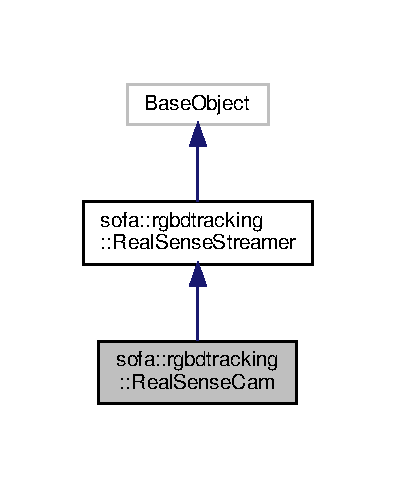
\includegraphics[width=190pt]{classsofa_1_1rgbdtracking_1_1_real_sense_cam__inherit__graph}
\end{center}
\end{figure}


Collaboration diagram for sofa\+:\+:rgbdtracking\+:\+:Real\+Sense\+Cam\+:
\nopagebreak
\begin{figure}[H]
\begin{center}
\leavevmode
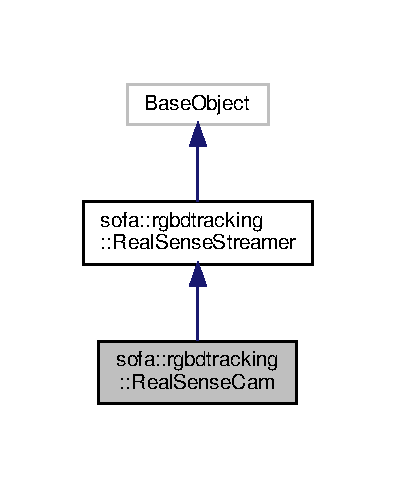
\includegraphics[width=190pt]{classsofa_1_1rgbdtracking_1_1_real_sense_cam__coll__graph}
\end{center}
\end{figure}
\subsection*{Public Types}
\begin{DoxyCompactItemize}
\item 
\mbox{\Hypertarget{classsofa_1_1rgbdtracking_1_1_real_sense_cam_a0a77e286d896d3e917359d3e7a3d6c47}\label{classsofa_1_1rgbdtracking_1_1_real_sense_cam_a0a77e286d896d3e917359d3e7a3d6c47}} 
typedef \hyperlink{classsofa_1_1rgbdtracking_1_1_real_sense_streamer}{Real\+Sense\+Streamer} {\bfseries Inherited}
\end{DoxyCompactItemize}
\subsection*{Public Member Functions}
\begin{DoxyCompactItemize}
\item 
\mbox{\Hypertarget{classsofa_1_1rgbdtracking_1_1_real_sense_cam_a32f3a2ac2480dba52c84620583c4d6e3}\label{classsofa_1_1rgbdtracking_1_1_real_sense_cam_a32f3a2ac2480dba52c84620583c4d6e3}} 
{\bfseries S\+O\+F\+A\+\_\+\+C\+L\+A\+SS} (\hyperlink{classsofa_1_1rgbdtracking_1_1_real_sense_cam}{Real\+Sense\+Cam}, \hyperlink{classsofa_1_1rgbdtracking_1_1_real_sense_streamer}{Real\+Sense\+Streamer})
\item 
\mbox{\Hypertarget{classsofa_1_1rgbdtracking_1_1_real_sense_cam_af0fc64dd75ab34819f1341ce97359634}\label{classsofa_1_1rgbdtracking_1_1_real_sense_cam_af0fc64dd75ab34819f1341ce97359634}} 
void {\bfseries decode\+Image} (cv\+::\+Mat \&img)
\item 
\mbox{\Hypertarget{classsofa_1_1rgbdtracking_1_1_real_sense_cam_abf95b6b7d177c8718c779947e1a19bdc}\label{classsofa_1_1rgbdtracking_1_1_real_sense_cam_abf95b6b7d177c8718c779947e1a19bdc}} 
void {\bfseries handle\+Event} (sofa\+::core\+::objectmodel\+::\+Event $\ast$event)
\end{DoxyCompactItemize}
\subsection*{Public Attributes}
\begin{DoxyCompactItemize}
\item 
\mbox{\Hypertarget{classsofa_1_1rgbdtracking_1_1_real_sense_cam_a44e727c66935e408f2ba4de6e0699b6b}\label{classsofa_1_1rgbdtracking_1_1_real_sense_cam_a44e727c66935e408f2ba4de6e0699b6b}} 
Data$<$ int $>$ {\bfseries depth\+Mode}
\item 
\mbox{\Hypertarget{classsofa_1_1rgbdtracking_1_1_real_sense_cam_ad605d7bbc20faee2b716df53474412dc}\label{classsofa_1_1rgbdtracking_1_1_real_sense_cam_ad605d7bbc20faee2b716df53474412dc}} 
Data$<$ opencvplugin\+::\+Track\+Bar1 $>$ {\bfseries d\+\_\+exposure}
\item 
\mbox{\Hypertarget{classsofa_1_1rgbdtracking_1_1_real_sense_cam_a67ec547de6f69bebef2a7f2e8d584f48}\label{classsofa_1_1rgbdtracking_1_1_real_sense_cam_a67ec547de6f69bebef2a7f2e8d584f48}} 
Data\+Callback {\bfseries c\+\_\+exposure}
\item 
\mbox{\Hypertarget{classsofa_1_1rgbdtracking_1_1_real_sense_cam_a07b608dff4127a1ea22ffcc93a0a2b8b}\label{classsofa_1_1rgbdtracking_1_1_real_sense_cam_a07b608dff4127a1ea22ffcc93a0a2b8b}} 
rs2\+\_\+intrinsics {\bfseries cam\+\_\+intrinsics}
\item 
\mbox{\Hypertarget{classsofa_1_1rgbdtracking_1_1_real_sense_cam_a9c40355cbe2db5d7ccd20a6ff3d6c8d2}\label{classsofa_1_1rgbdtracking_1_1_real_sense_cam_a9c40355cbe2db5d7ccd20a6ff3d6c8d2}} 
rs2\+::pipeline\+\_\+profile {\bfseries selection}
\item 
\mbox{\Hypertarget{classsofa_1_1rgbdtracking_1_1_real_sense_cam_a622f15e0a08312b92571bd5c4d040ea1}\label{classsofa_1_1rgbdtracking_1_1_real_sense_cam_a622f15e0a08312b92571bd5c4d040ea1}} 
rs2\+::pointcloud \hyperlink{classsofa_1_1rgbdtracking_1_1_real_sense_cam_a622f15e0a08312b92571bd5c4d040ea1}{pc}
\begin{DoxyCompactList}\small\item\em for pointcloud extraction, deprecated \end{DoxyCompactList}\item 
\mbox{\Hypertarget{classsofa_1_1rgbdtracking_1_1_real_sense_cam_a4fbb2690c02fea1635913680e08efd7b}\label{classsofa_1_1rgbdtracking_1_1_real_sense_cam_a4fbb2690c02fea1635913680e08efd7b}} 
rs2\+::points {\bfseries points}
\item 
\mbox{\Hypertarget{classsofa_1_1rgbdtracking_1_1_real_sense_cam_a630e600956571e553972403bba7fcf02}\label{classsofa_1_1rgbdtracking_1_1_real_sense_cam_a630e600956571e553972403bba7fcf02}} 
rs2\+::pipeline \hyperlink{classsofa_1_1rgbdtracking_1_1_real_sense_cam_a630e600956571e553972403bba7fcf02}{pipe}
\begin{DoxyCompactList}\small\item\em Real\+Sense pipeline, encapsulating the actual device and sensors. \end{DoxyCompactList}\item 
\mbox{\Hypertarget{classsofa_1_1rgbdtracking_1_1_real_sense_cam_a9fce91c3e7d2c1be3aaca521ea28d14f}\label{classsofa_1_1rgbdtracking_1_1_real_sense_cam_a9fce91c3e7d2c1be3aaca521ea28d14f}} 
bool {\bfseries pause}
\end{DoxyCompactItemize}
\subsection*{Protected Member Functions}
\begin{DoxyCompactItemize}
\item 
\mbox{\Hypertarget{classsofa_1_1rgbdtracking_1_1_real_sense_cam_ad11af2a678cdbe9d4cb69160654ddc59}\label{classsofa_1_1rgbdtracking_1_1_real_sense_cam_ad11af2a678cdbe9d4cb69160654ddc59}} 
void \hyperlink{classsofa_1_1rgbdtracking_1_1_real_sense_cam_ad11af2a678cdbe9d4cb69160654ddc59}{set\+Exposure} ()
\begin{DoxyCompactList}\small\item\em set exposure of camera from \char`\"{}exposure\char`\"{} data in sofa \end{DoxyCompactList}\item 
\mbox{\Hypertarget{classsofa_1_1rgbdtracking_1_1_real_sense_cam_a60647ccc41e670ac3f5d7ad8b5d96194}\label{classsofa_1_1rgbdtracking_1_1_real_sense_cam_a60647ccc41e670ac3f5d7ad8b5d96194}} 
void \hyperlink{classsofa_1_1rgbdtracking_1_1_real_sense_cam_a60647ccc41e670ac3f5d7ad8b5d96194}{config\+Pipe} ()
\begin{DoxyCompactList}\small\item\em setup realsense data acquisition pipeline \end{DoxyCompactList}\item 
\mbox{\Hypertarget{classsofa_1_1rgbdtracking_1_1_real_sense_cam_a90411168a51a6899f412391bfae3b7ed}\label{classsofa_1_1rgbdtracking_1_1_real_sense_cam_a90411168a51a6899f412391bfae3b7ed}} 
void \hyperlink{classsofa_1_1rgbdtracking_1_1_real_sense_cam_a90411168a51a6899f412391bfae3b7ed}{stabilize\+Auto\+Exp} ()
\begin{DoxyCompactList}\small\item\em wait for a second in order for auto exposure to settle in at initialization \end{DoxyCompactList}\item 
\mbox{\Hypertarget{classsofa_1_1rgbdtracking_1_1_real_sense_cam_a617df3395a331f0e4a046da1c79ab8f0}\label{classsofa_1_1rgbdtracking_1_1_real_sense_cam_a617df3395a331f0e4a046da1c79ab8f0}} 
void {\bfseries init} ()
\item 
\mbox{\Hypertarget{classsofa_1_1rgbdtracking_1_1_real_sense_cam_a29789038ece88a4d6485c0f6d01abe70}\label{classsofa_1_1rgbdtracking_1_1_real_sense_cam_a29789038ece88a4d6485c0f6d01abe70}} 
void {\bfseries acquire\+Aligned} (cv\+::\+Mat \&img)
\item 
\mbox{\Hypertarget{classsofa_1_1rgbdtracking_1_1_real_sense_cam_a14c83fdb652f4d40a95a402dd930f7a9}\label{classsofa_1_1rgbdtracking_1_1_real_sense_cam_a14c83fdb652f4d40a95a402dd930f7a9}} 
void {\bfseries getpointcloud} (rs2\+::frame color, rs2\+::frame depth)
\end{DoxyCompactItemize}


\subsection{Detailed Description}
The \hyperlink{classsofa_1_1rgbdtracking_1_1_real_sense_cam}{Real\+Sense\+Cam} class Streamer to use when only one realsense is connected. 

The documentation for this class was generated from the following file\+:\begin{DoxyCompactItemize}
\item 
src/sofa/realsenseplugin/streamer/Real\+Sense\+Cam.\+h\end{DoxyCompactItemize}

\hypertarget{classsofa_1_1rgbdtracking_1_1_real_sense_deprojector}{}\section{sofa\+:\+:rgbdtracking\+:\+:Real\+Sense\+Deprojector Class Reference}
\label{classsofa_1_1rgbdtracking_1_1_real_sense_deprojector}\index{sofa\+::rgbdtracking\+::\+Real\+Sense\+Deprojector@{sofa\+::rgbdtracking\+::\+Real\+Sense\+Deprojector}}


The \hyperlink{classsofa_1_1rgbdtracking_1_1_real_sense_deprojector}{Real\+Sense\+Deprojector} class Online / Offline 2\+D-\/3D deprojection of whole rgb-\/d scene.  




{\ttfamily \#include $<$Real\+Sense\+Deprojector.\+h$>$}



Inheritance diagram for sofa\+:\+:rgbdtracking\+:\+:Real\+Sense\+Deprojector\+:\nopagebreak
\begin{figure}[H]
\begin{center}
\leavevmode
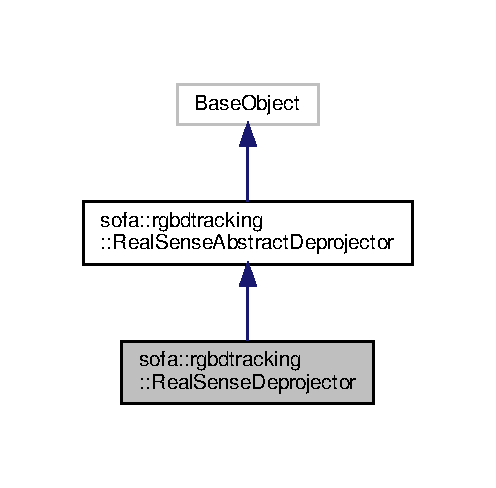
\includegraphics[width=238pt]{classsofa_1_1rgbdtracking_1_1_real_sense_deprojector__inherit__graph}
\end{center}
\end{figure}


Collaboration diagram for sofa\+:\+:rgbdtracking\+:\+:Real\+Sense\+Deprojector\+:\nopagebreak
\begin{figure}[H]
\begin{center}
\leavevmode
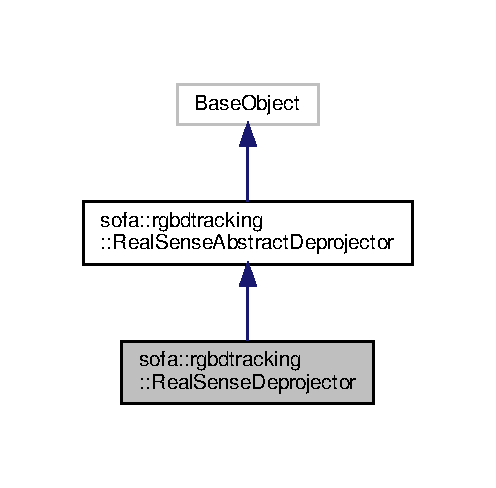
\includegraphics[width=238pt]{classsofa_1_1rgbdtracking_1_1_real_sense_deprojector__coll__graph}
\end{center}
\end{figure}
\subsection*{Public Types}
\begin{DoxyCompactItemize}
\item 
\mbox{\Hypertarget{classsofa_1_1rgbdtracking_1_1_real_sense_deprojector_a6bae03808ffd8dcb3a90e7ed450cac45}\label{classsofa_1_1rgbdtracking_1_1_real_sense_deprojector_a6bae03808ffd8dcb3a90e7ed450cac45}} 
typedef \hyperlink{classsofa_1_1rgbdtracking_1_1_real_sense_abstract_deprojector}{Real\+Sense\+Abstract\+Deprojector} {\bfseries Inherited}
\end{DoxyCompactItemize}
\subsection*{Public Member Functions}
\begin{DoxyCompactItemize}
\item 
\mbox{\Hypertarget{classsofa_1_1rgbdtracking_1_1_real_sense_deprojector_ab83880605bbf09764e64573381b5502c}\label{classsofa_1_1rgbdtracking_1_1_real_sense_deprojector_ab83880605bbf09764e64573381b5502c}} 
{\bfseries S\+O\+F\+A\+\_\+\+C\+L\+A\+SS} (\hyperlink{classsofa_1_1rgbdtracking_1_1_real_sense_deprojector}{Real\+Sense\+Deprojector}, Inherited)
\item 
void \hyperlink{classsofa_1_1rgbdtracking_1_1_real_sense_deprojector_aaa5648b58d79dcabc8265d7eec19b78a}{handle\+Event} (sofa\+::core\+::objectmodel\+::\+Event $\ast$event)
\begin{DoxyCompactList}\small\item\em handle\+Event \+: Press P to export 3D snapshot of current frame \end{DoxyCompactList}\end{DoxyCompactItemize}
\subsection*{Public Attributes}
\begin{DoxyCompactItemize}
\item 
\mbox{\Hypertarget{classsofa_1_1rgbdtracking_1_1_real_sense_deprojector_a61d80c84f736effdb2ecbd41000b1bea}\label{classsofa_1_1rgbdtracking_1_1_real_sense_deprojector_a61d80c84f736effdb2ecbd41000b1bea}} 
Data$<$ opencvplugin\+::\+Image\+Data $>$ \hyperlink{classsofa_1_1rgbdtracking_1_1_real_sense_deprojector_a61d80c84f736effdb2ecbd41000b1bea}{d\+\_\+color}
\begin{DoxyCompactList}\small\item\em color frame for snapshot exportation \end{DoxyCompactList}\item 
\mbox{\Hypertarget{classsofa_1_1rgbdtracking_1_1_real_sense_deprojector_ae6f6cf6fff6c3cc81e1370d17b627395}\label{classsofa_1_1rgbdtracking_1_1_real_sense_deprojector_ae6f6cf6fff6c3cc81e1370d17b627395}} 
Data$<$ std\+::string $>$ \hyperlink{classsofa_1_1rgbdtracking_1_1_real_sense_deprojector_ae6f6cf6fff6c3cc81e1370d17b627395}{d\+\_\+snap\+\_\+path}
\begin{DoxyCompactList}\small\item\em path to save snapshots to \end{DoxyCompactList}\item 
\mbox{\Hypertarget{classsofa_1_1rgbdtracking_1_1_real_sense_deprojector_a718873322b7771e3ddf7fa1da705ca6f}\label{classsofa_1_1rgbdtracking_1_1_real_sense_deprojector_a718873322b7771e3ddf7fa1da705ca6f}} 
Data\+Callback {\bfseries c\+\_\+image}
\end{DoxyCompactItemize}


\subsection{Detailed Description}
The \hyperlink{classsofa_1_1rgbdtracking_1_1_real_sense_deprojector}{Real\+Sense\+Deprojector} class Online / Offline 2\+D-\/3D deprojection of whole rgb-\/d scene. 

\subsection{Member Function Documentation}
\mbox{\Hypertarget{classsofa_1_1rgbdtracking_1_1_real_sense_deprojector_aaa5648b58d79dcabc8265d7eec19b78a}\label{classsofa_1_1rgbdtracking_1_1_real_sense_deprojector_aaa5648b58d79dcabc8265d7eec19b78a}} 
\index{sofa\+::rgbdtracking\+::\+Real\+Sense\+Deprojector@{sofa\+::rgbdtracking\+::\+Real\+Sense\+Deprojector}!handle\+Event@{handle\+Event}}
\index{handle\+Event@{handle\+Event}!sofa\+::rgbdtracking\+::\+Real\+Sense\+Deprojector@{sofa\+::rgbdtracking\+::\+Real\+Sense\+Deprojector}}
\subsubsection{\texorpdfstring{handle\+Event()}{handleEvent()}}
{\footnotesize\ttfamily void sofa\+::rgbdtracking\+::\+Real\+Sense\+Deprojector\+::handle\+Event (\begin{DoxyParamCaption}\item[{sofa\+::core\+::objectmodel\+::\+Event $\ast$}]{event }\end{DoxyParamCaption})\hspace{0.3cm}{\ttfamily [inline]}}



handle\+Event \+: Press P to export 3D snapshot of current frame 


\begin{DoxyParams}{Parameters}
{\em event} & \\
\hline
\end{DoxyParams}


The documentation for this class was generated from the following file\+:\begin{DoxyCompactItemize}
\item 
src/sofa/realsenseplugin/projector/Real\+Sense\+Deprojector.\+h\end{DoxyCompactItemize}

\hypertarget{classsofa_1_1rgbdtracking_1_1_real_sense_dist_frame}{}\section{sofa\+:\+:rgbdtracking\+:\+:Real\+Sense\+Dist\+Frame Class Reference}
\label{classsofa_1_1rgbdtracking_1_1_real_sense_dist_frame}\index{sofa\+::rgbdtracking\+::\+Real\+Sense\+Dist\+Frame@{sofa\+::rgbdtracking\+::\+Real\+Sense\+Dist\+Frame}}


The \hyperlink{classsofa_1_1rgbdtracking_1_1_real_sense_dist_frame}{Real\+Sense\+Dist\+Frame} class Used for distance frame usage as sofa data by components.  




{\ttfamily \#include $<$Real\+Sense\+Dist\+Frame.\+h$>$}



Collaboration diagram for sofa\+:\+:rgbdtracking\+:\+:Real\+Sense\+Dist\+Frame\+:\nopagebreak
\begin{figure}[H]
\begin{center}
\leavevmode
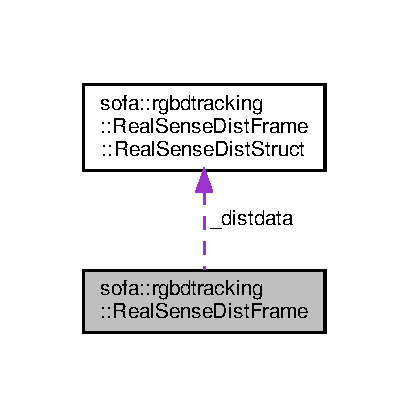
\includegraphics[width=196pt]{classsofa_1_1rgbdtracking_1_1_real_sense_dist_frame__coll__graph}
\end{center}
\end{figure}
\subsection*{Classes}
\begin{DoxyCompactItemize}
\item 
struct \hyperlink{structsofa_1_1rgbdtracking_1_1_real_sense_dist_frame_1_1_real_sense_dist_struct}{Real\+Sense\+Dist\+Struct}
\end{DoxyCompactItemize}
\subsection*{Public Member Functions}
\begin{DoxyCompactItemize}
\item 
\hyperlink{classsofa_1_1rgbdtracking_1_1_real_sense_dist_frame_a3d49568e24334c3381cc363987bcf459}{Real\+Sense\+Dist\+Frame} ()
\item 
\hyperlink{classsofa_1_1rgbdtracking_1_1_real_sense_dist_frame_ae2a25fc1045c2dd511e7ccdaa2ad0f04}{Real\+Sense\+Dist\+Frame} (\hyperlink{structsofa_1_1rgbdtracking_1_1_real_sense_dist_frame_1_1_real_sense_dist_struct}{Real\+Sense\+Dist\+Struct} diststr)
\item 
\hyperlink{classsofa_1_1rgbdtracking_1_1_real_sense_dist_frame_a6bea0bb06a130b94dc9066c60a22a4e1}{operator Real\+Sense\+Dist\+Struct \&} ()
\item 
\hyperlink{classsofa_1_1rgbdtracking_1_1_real_sense_dist_frame_adf4c6fd68dd4a70e21bdb90b7ee9e562}{operator const Real\+Sense\+Dist\+Struct \&} ()
\item 
size\+\_\+t \hyperlink{classsofa_1_1rgbdtracking_1_1_real_sense_dist_frame_a95d9d7721c43df3754b482467062dfe9}{width} () const
\item 
size\+\_\+t \hyperlink{classsofa_1_1rgbdtracking_1_1_real_sense_dist_frame_ac2ced1d45e4ad6845d78550b196bbab1}{height} () const
\item 
float $\ast$ \hyperlink{classsofa_1_1rgbdtracking_1_1_real_sense_dist_frame_a0b624e4794f1dc10b49c90b99748cf89}{data} ()
\item 
\hyperlink{structsofa_1_1rgbdtracking_1_1_real_sense_dist_frame_1_1_real_sense_dist_struct}{Real\+Sense\+Dist\+Struct} \& \hyperlink{classsofa_1_1rgbdtracking_1_1_real_sense_dist_frame_aaab7f670c0ce70e409c298922d9d5afe}{get\+Frame} ()
\end{DoxyCompactItemize}
\subsection*{Public Attributes}
\begin{DoxyCompactItemize}
\item 
\hyperlink{structsofa_1_1rgbdtracking_1_1_real_sense_dist_frame_1_1_real_sense_dist_struct}{Real\+Sense\+Dist\+Struct} \hyperlink{classsofa_1_1rgbdtracking_1_1_real_sense_dist_frame_a95575d91b20d0cdc8cb9a9ba3795f928}{\+\_\+distdata}
\end{DoxyCompactItemize}
\subsection*{Friends}
\begin{DoxyCompactItemize}
\item 
std\+::istream \& \hyperlink{classsofa_1_1rgbdtracking_1_1_real_sense_dist_frame_ac7776007f9ac565bc64143b9c2e29c7d}{operator$>$$>$} (std\+::istream \&in, \hyperlink{classsofa_1_1rgbdtracking_1_1_real_sense_dist_frame}{Real\+Sense\+Dist\+Frame} \&)
\item 
std\+::ostream \& \hyperlink{classsofa_1_1rgbdtracking_1_1_real_sense_dist_frame_ad9831ad196082e583b86e863ec7d3460}{operator$<$$<$} (std\+::ostream \&out, const \hyperlink{classsofa_1_1rgbdtracking_1_1_real_sense_dist_frame}{Real\+Sense\+Dist\+Frame} \&)
\end{DoxyCompactItemize}


\subsection{Detailed Description}
The \hyperlink{classsofa_1_1rgbdtracking_1_1_real_sense_dist_frame}{Real\+Sense\+Dist\+Frame} class Used for distance frame usage as sofa data by components. 

\subsection{Constructor \& Destructor Documentation}
\mbox{\Hypertarget{classsofa_1_1rgbdtracking_1_1_real_sense_dist_frame_a3d49568e24334c3381cc363987bcf459}\label{classsofa_1_1rgbdtracking_1_1_real_sense_dist_frame_a3d49568e24334c3381cc363987bcf459}} 
\index{sofa\+::rgbdtracking\+::\+Real\+Sense\+Dist\+Frame@{sofa\+::rgbdtracking\+::\+Real\+Sense\+Dist\+Frame}!Real\+Sense\+Dist\+Frame@{Real\+Sense\+Dist\+Frame}}
\index{Real\+Sense\+Dist\+Frame@{Real\+Sense\+Dist\+Frame}!sofa\+::rgbdtracking\+::\+Real\+Sense\+Dist\+Frame@{sofa\+::rgbdtracking\+::\+Real\+Sense\+Dist\+Frame}}
\subsubsection{\texorpdfstring{Real\+Sense\+Dist\+Frame()}{RealSenseDistFrame()}\hspace{0.1cm}{\footnotesize\ttfamily [1/2]}}
{\footnotesize\ttfamily sofa\+::rgbdtracking\+::\+Real\+Sense\+Dist\+Frame\+::\+Real\+Sense\+Dist\+Frame (\begin{DoxyParamCaption}{ }\end{DoxyParamCaption})\hspace{0.3cm}{\ttfamily [inline]}}

\mbox{\Hypertarget{classsofa_1_1rgbdtracking_1_1_real_sense_dist_frame_ae2a25fc1045c2dd511e7ccdaa2ad0f04}\label{classsofa_1_1rgbdtracking_1_1_real_sense_dist_frame_ae2a25fc1045c2dd511e7ccdaa2ad0f04}} 
\index{sofa\+::rgbdtracking\+::\+Real\+Sense\+Dist\+Frame@{sofa\+::rgbdtracking\+::\+Real\+Sense\+Dist\+Frame}!Real\+Sense\+Dist\+Frame@{Real\+Sense\+Dist\+Frame}}
\index{Real\+Sense\+Dist\+Frame@{Real\+Sense\+Dist\+Frame}!sofa\+::rgbdtracking\+::\+Real\+Sense\+Dist\+Frame@{sofa\+::rgbdtracking\+::\+Real\+Sense\+Dist\+Frame}}
\subsubsection{\texorpdfstring{Real\+Sense\+Dist\+Frame()}{RealSenseDistFrame()}\hspace{0.1cm}{\footnotesize\ttfamily [2/2]}}
{\footnotesize\ttfamily sofa\+::rgbdtracking\+::\+Real\+Sense\+Dist\+Frame\+::\+Real\+Sense\+Dist\+Frame (\begin{DoxyParamCaption}\item[{\hyperlink{structsofa_1_1rgbdtracking_1_1_real_sense_dist_frame_1_1_real_sense_dist_struct}{Real\+Sense\+Dist\+Struct}}]{diststr }\end{DoxyParamCaption})\hspace{0.3cm}{\ttfamily [inline]}}



\subsection{Member Function Documentation}
\mbox{\Hypertarget{classsofa_1_1rgbdtracking_1_1_real_sense_dist_frame_a0b624e4794f1dc10b49c90b99748cf89}\label{classsofa_1_1rgbdtracking_1_1_real_sense_dist_frame_a0b624e4794f1dc10b49c90b99748cf89}} 
\index{sofa\+::rgbdtracking\+::\+Real\+Sense\+Dist\+Frame@{sofa\+::rgbdtracking\+::\+Real\+Sense\+Dist\+Frame}!data@{data}}
\index{data@{data}!sofa\+::rgbdtracking\+::\+Real\+Sense\+Dist\+Frame@{sofa\+::rgbdtracking\+::\+Real\+Sense\+Dist\+Frame}}
\subsubsection{\texorpdfstring{data()}{data()}}
{\footnotesize\ttfamily float$\ast$ sofa\+::rgbdtracking\+::\+Real\+Sense\+Dist\+Frame\+::data (\begin{DoxyParamCaption}{ }\end{DoxyParamCaption})\hspace{0.3cm}{\ttfamily [inline]}}

\mbox{\Hypertarget{classsofa_1_1rgbdtracking_1_1_real_sense_dist_frame_aaab7f670c0ce70e409c298922d9d5afe}\label{classsofa_1_1rgbdtracking_1_1_real_sense_dist_frame_aaab7f670c0ce70e409c298922d9d5afe}} 
\index{sofa\+::rgbdtracking\+::\+Real\+Sense\+Dist\+Frame@{sofa\+::rgbdtracking\+::\+Real\+Sense\+Dist\+Frame}!get\+Frame@{get\+Frame}}
\index{get\+Frame@{get\+Frame}!sofa\+::rgbdtracking\+::\+Real\+Sense\+Dist\+Frame@{sofa\+::rgbdtracking\+::\+Real\+Sense\+Dist\+Frame}}
\subsubsection{\texorpdfstring{get\+Frame()}{getFrame()}}
{\footnotesize\ttfamily \hyperlink{structsofa_1_1rgbdtracking_1_1_real_sense_dist_frame_1_1_real_sense_dist_struct}{Real\+Sense\+Dist\+Struct}\& sofa\+::rgbdtracking\+::\+Real\+Sense\+Dist\+Frame\+::get\+Frame (\begin{DoxyParamCaption}{ }\end{DoxyParamCaption})\hspace{0.3cm}{\ttfamily [inline]}}

\mbox{\Hypertarget{classsofa_1_1rgbdtracking_1_1_real_sense_dist_frame_ac2ced1d45e4ad6845d78550b196bbab1}\label{classsofa_1_1rgbdtracking_1_1_real_sense_dist_frame_ac2ced1d45e4ad6845d78550b196bbab1}} 
\index{sofa\+::rgbdtracking\+::\+Real\+Sense\+Dist\+Frame@{sofa\+::rgbdtracking\+::\+Real\+Sense\+Dist\+Frame}!height@{height}}
\index{height@{height}!sofa\+::rgbdtracking\+::\+Real\+Sense\+Dist\+Frame@{sofa\+::rgbdtracking\+::\+Real\+Sense\+Dist\+Frame}}
\subsubsection{\texorpdfstring{height()}{height()}}
{\footnotesize\ttfamily size\+\_\+t sofa\+::rgbdtracking\+::\+Real\+Sense\+Dist\+Frame\+::height (\begin{DoxyParamCaption}{ }\end{DoxyParamCaption}) const\hspace{0.3cm}{\ttfamily [inline]}}

\mbox{\Hypertarget{classsofa_1_1rgbdtracking_1_1_real_sense_dist_frame_adf4c6fd68dd4a70e21bdb90b7ee9e562}\label{classsofa_1_1rgbdtracking_1_1_real_sense_dist_frame_adf4c6fd68dd4a70e21bdb90b7ee9e562}} 
\index{sofa\+::rgbdtracking\+::\+Real\+Sense\+Dist\+Frame@{sofa\+::rgbdtracking\+::\+Real\+Sense\+Dist\+Frame}!operator const Real\+Sense\+Dist\+Struct \&@{operator const Real\+Sense\+Dist\+Struct \&}}
\index{operator const Real\+Sense\+Dist\+Struct \&@{operator const Real\+Sense\+Dist\+Struct \&}!sofa\+::rgbdtracking\+::\+Real\+Sense\+Dist\+Frame@{sofa\+::rgbdtracking\+::\+Real\+Sense\+Dist\+Frame}}
\subsubsection{\texorpdfstring{operator const Real\+Sense\+Dist\+Struct \&()}{operator const RealSenseDistStruct \&()}}
{\footnotesize\ttfamily sofa\+::rgbdtracking\+::\+Real\+Sense\+Dist\+Frame\+::operator const \hyperlink{structsofa_1_1rgbdtracking_1_1_real_sense_dist_frame_1_1_real_sense_dist_struct}{Real\+Sense\+Dist\+Struct} \& (\begin{DoxyParamCaption}{ }\end{DoxyParamCaption})\hspace{0.3cm}{\ttfamily [inline]}}

\mbox{\Hypertarget{classsofa_1_1rgbdtracking_1_1_real_sense_dist_frame_a6bea0bb06a130b94dc9066c60a22a4e1}\label{classsofa_1_1rgbdtracking_1_1_real_sense_dist_frame_a6bea0bb06a130b94dc9066c60a22a4e1}} 
\index{sofa\+::rgbdtracking\+::\+Real\+Sense\+Dist\+Frame@{sofa\+::rgbdtracking\+::\+Real\+Sense\+Dist\+Frame}!operator Real\+Sense\+Dist\+Struct \&@{operator Real\+Sense\+Dist\+Struct \&}}
\index{operator Real\+Sense\+Dist\+Struct \&@{operator Real\+Sense\+Dist\+Struct \&}!sofa\+::rgbdtracking\+::\+Real\+Sense\+Dist\+Frame@{sofa\+::rgbdtracking\+::\+Real\+Sense\+Dist\+Frame}}
\subsubsection{\texorpdfstring{operator Real\+Sense\+Dist\+Struct \&()}{operator RealSenseDistStruct \&()}}
{\footnotesize\ttfamily sofa\+::rgbdtracking\+::\+Real\+Sense\+Dist\+Frame\+::operator \hyperlink{structsofa_1_1rgbdtracking_1_1_real_sense_dist_frame_1_1_real_sense_dist_struct}{Real\+Sense\+Dist\+Struct} \& (\begin{DoxyParamCaption}{ }\end{DoxyParamCaption})\hspace{0.3cm}{\ttfamily [inline]}}

\mbox{\Hypertarget{classsofa_1_1rgbdtracking_1_1_real_sense_dist_frame_a95d9d7721c43df3754b482467062dfe9}\label{classsofa_1_1rgbdtracking_1_1_real_sense_dist_frame_a95d9d7721c43df3754b482467062dfe9}} 
\index{sofa\+::rgbdtracking\+::\+Real\+Sense\+Dist\+Frame@{sofa\+::rgbdtracking\+::\+Real\+Sense\+Dist\+Frame}!width@{width}}
\index{width@{width}!sofa\+::rgbdtracking\+::\+Real\+Sense\+Dist\+Frame@{sofa\+::rgbdtracking\+::\+Real\+Sense\+Dist\+Frame}}
\subsubsection{\texorpdfstring{width()}{width()}}
{\footnotesize\ttfamily size\+\_\+t sofa\+::rgbdtracking\+::\+Real\+Sense\+Dist\+Frame\+::width (\begin{DoxyParamCaption}{ }\end{DoxyParamCaption}) const\hspace{0.3cm}{\ttfamily [inline]}}



\subsection{Friends And Related Function Documentation}
\mbox{\Hypertarget{classsofa_1_1rgbdtracking_1_1_real_sense_dist_frame_ad9831ad196082e583b86e863ec7d3460}\label{classsofa_1_1rgbdtracking_1_1_real_sense_dist_frame_ad9831ad196082e583b86e863ec7d3460}} 
\index{sofa\+::rgbdtracking\+::\+Real\+Sense\+Dist\+Frame@{sofa\+::rgbdtracking\+::\+Real\+Sense\+Dist\+Frame}!operator$<$$<$@{operator$<$$<$}}
\index{operator$<$$<$@{operator$<$$<$}!sofa\+::rgbdtracking\+::\+Real\+Sense\+Dist\+Frame@{sofa\+::rgbdtracking\+::\+Real\+Sense\+Dist\+Frame}}
\subsubsection{\texorpdfstring{operator$<$$<$}{operator<<}}
{\footnotesize\ttfamily std\+::ostream\& operator$<$$<$ (\begin{DoxyParamCaption}\item[{std\+::ostream \&}]{out,  }\item[{const \hyperlink{classsofa_1_1rgbdtracking_1_1_real_sense_dist_frame}{Real\+Sense\+Dist\+Frame} \&}]{ }\end{DoxyParamCaption})\hspace{0.3cm}{\ttfamily [friend]}}

\mbox{\Hypertarget{classsofa_1_1rgbdtracking_1_1_real_sense_dist_frame_ac7776007f9ac565bc64143b9c2e29c7d}\label{classsofa_1_1rgbdtracking_1_1_real_sense_dist_frame_ac7776007f9ac565bc64143b9c2e29c7d}} 
\index{sofa\+::rgbdtracking\+::\+Real\+Sense\+Dist\+Frame@{sofa\+::rgbdtracking\+::\+Real\+Sense\+Dist\+Frame}!operator$>$$>$@{operator$>$$>$}}
\index{operator$>$$>$@{operator$>$$>$}!sofa\+::rgbdtracking\+::\+Real\+Sense\+Dist\+Frame@{sofa\+::rgbdtracking\+::\+Real\+Sense\+Dist\+Frame}}
\subsubsection{\texorpdfstring{operator$>$$>$}{operator>>}}
{\footnotesize\ttfamily std\+::istream\& operator$>$$>$ (\begin{DoxyParamCaption}\item[{std\+::istream \&}]{in,  }\item[{\hyperlink{classsofa_1_1rgbdtracking_1_1_real_sense_dist_frame}{Real\+Sense\+Dist\+Frame} \&}]{ }\end{DoxyParamCaption})\hspace{0.3cm}{\ttfamily [friend]}}



\subsection{Member Data Documentation}
\mbox{\Hypertarget{classsofa_1_1rgbdtracking_1_1_real_sense_dist_frame_a95575d91b20d0cdc8cb9a9ba3795f928}\label{classsofa_1_1rgbdtracking_1_1_real_sense_dist_frame_a95575d91b20d0cdc8cb9a9ba3795f928}} 
\index{sofa\+::rgbdtracking\+::\+Real\+Sense\+Dist\+Frame@{sofa\+::rgbdtracking\+::\+Real\+Sense\+Dist\+Frame}!\+\_\+distdata@{\+\_\+distdata}}
\index{\+\_\+distdata@{\+\_\+distdata}!sofa\+::rgbdtracking\+::\+Real\+Sense\+Dist\+Frame@{sofa\+::rgbdtracking\+::\+Real\+Sense\+Dist\+Frame}}
\subsubsection{\texorpdfstring{\+\_\+distdata}{\_distdata}}
{\footnotesize\ttfamily \hyperlink{structsofa_1_1rgbdtracking_1_1_real_sense_dist_frame_1_1_real_sense_dist_struct}{Real\+Sense\+Dist\+Struct} sofa\+::rgbdtracking\+::\+Real\+Sense\+Dist\+Frame\+::\+\_\+distdata}



The documentation for this class was generated from the following file\+:\begin{DoxyCompactItemize}
\item 
src/sofa/realsenseplugin/projector/\hyperlink{_real_sense_dist_frame_8h}{Real\+Sense\+Dist\+Frame.\+h}\end{DoxyCompactItemize}

\hypertarget{classsofa_1_1rgbdtracking_1_1_real_sense_dist_frame_exporter}{}\section{sofa\+:\+:rgbdtracking\+:\+:Real\+Sense\+Dist\+Frame\+Exporter Class Reference}
\label{classsofa_1_1rgbdtracking_1_1_real_sense_dist_frame_exporter}\index{sofa\+::rgbdtracking\+::\+Real\+Sense\+Dist\+Frame\+Exporter@{sofa\+::rgbdtracking\+::\+Real\+Sense\+Dist\+Frame\+Exporter}}


The \hyperlink{classsofa_1_1rgbdtracking_1_1_real_sense_dist_frame_exporter}{Real\+Sense\+Dist\+Frame\+Exporter} class exports distance frames to file for offline processing.  




{\ttfamily \#include $<$Real\+Sense\+Dist\+Frame.\+h$>$}



Inheritance diagram for sofa\+:\+:rgbdtracking\+:\+:Real\+Sense\+Dist\+Frame\+Exporter\+:\nopagebreak
\begin{figure}[H]
\begin{center}
\leavevmode
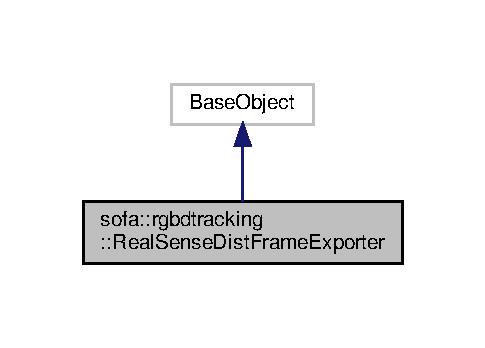
\includegraphics[width=233pt]{classsofa_1_1rgbdtracking_1_1_real_sense_dist_frame_exporter__inherit__graph}
\end{center}
\end{figure}


Collaboration diagram for sofa\+:\+:rgbdtracking\+:\+:Real\+Sense\+Dist\+Frame\+Exporter\+:\nopagebreak
\begin{figure}[H]
\begin{center}
\leavevmode
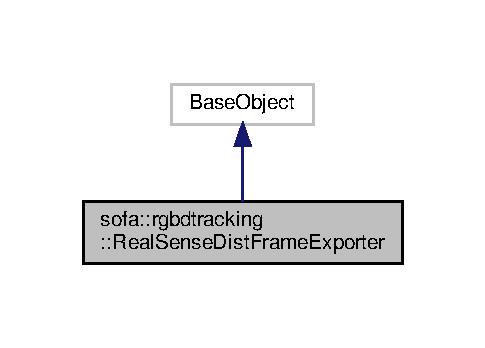
\includegraphics[width=233pt]{classsofa_1_1rgbdtracking_1_1_real_sense_dist_frame_exporter__coll__graph}
\end{center}
\end{figure}
\subsection*{Public Types}
\begin{DoxyCompactItemize}
\item 
typedef core\+::objectmodel\+::\+Base\+Object \hyperlink{classsofa_1_1rgbdtracking_1_1_real_sense_dist_frame_exporter_a3d5e841c18a10910a89dcaa8fafcaa53}{Inherited}
\end{DoxyCompactItemize}
\subsection*{Public Member Functions}
\begin{DoxyCompactItemize}
\item 
\hyperlink{classsofa_1_1rgbdtracking_1_1_real_sense_dist_frame_exporter_a4e09a848d4afe49248391a934c051eb5}{S\+O\+F\+A\+\_\+\+C\+L\+A\+SS} (\hyperlink{classsofa_1_1rgbdtracking_1_1_real_sense_dist_frame_exporter}{Real\+Sense\+Dist\+Frame\+Exporter}, core\+::objectmodel\+::\+Base\+Object)
\item 
\hyperlink{classsofa_1_1rgbdtracking_1_1_real_sense_dist_frame_exporter_a662756cddb128dfee5e6b7ceff636e68}{Real\+Sense\+Dist\+Frame\+Exporter} ()
\item 
\hyperlink{classsofa_1_1rgbdtracking_1_1_real_sense_dist_frame_exporter_af42acfd51a513b13ee2f70e6f4651b2e}{$\sim$\+Real\+Sense\+Dist\+Frame\+Exporter} ()
\item 
void \hyperlink{classsofa_1_1rgbdtracking_1_1_real_sense_dist_frame_exporter_af0422eedd90f9e7b8c5b17c33994a39c}{update\+File\+Stream} ()
\item 
void \hyperlink{classsofa_1_1rgbdtracking_1_1_real_sense_dist_frame_exporter_a97e36488ae57725cf05f28c1d70b18a3}{save\+Frame\+To\+Stream} ()
\begin{DoxyCompactList}\small\item\em write the frame in an opened binary file stream \end{DoxyCompactList}\item 
void \hyperlink{classsofa_1_1rgbdtracking_1_1_real_sense_dist_frame_exporter_ab788c5084fff8f6e8ee0d7b000af871b}{save\+Frame} ()
\begin{DoxyCompactList}\small\item\em Calledback each time distance frame changes. \end{DoxyCompactList}\item 
std\+::string \hyperlink{classsofa_1_1rgbdtracking_1_1_real_sense_dist_frame_exporter_aa5ebbe273df7d13fe9a8f648aa624d1c}{process\+File\+Name} ()
\end{DoxyCompactItemize}
\subsection*{Public Attributes}
\begin{DoxyCompactItemize}
\item 
Data$<$ std\+::string $>$ \hyperlink{classsofa_1_1rgbdtracking_1_1_real_sense_dist_frame_exporter_aa1e3e8aa4358ca07739f2c5977d5c895}{d\+\_\+filename}
\item 
\hyperlink{namespacesofa_1_1rgbdtracking_a00834a9204a667746fef9a402ccbfb55}{Data\+Callback} \hyperlink{classsofa_1_1rgbdtracking_1_1_real_sense_dist_frame_exporter_a6a6079ff7d5fdc6aaaab98359e25aba4}{c\+\_\+distframe}
\item 
Data$<$ \hyperlink{classsofa_1_1rgbdtracking_1_1_real_sense_dist_frame}{Real\+Sense\+Dist\+Frame} $>$ \hyperlink{classsofa_1_1rgbdtracking_1_1_real_sense_dist_frame_exporter_a452a048591840521dca0604336df2503}{d\+\_\+distframe}
\item 
\hyperlink{namespacesofa_1_1rgbdtracking_a00834a9204a667746fef9a402ccbfb55}{Data\+Callback} \hyperlink{classsofa_1_1rgbdtracking_1_1_real_sense_dist_frame_exporter_a1f2771b0bf0096dc0c9266f3a1916588}{c\+\_\+filename}
\item 
Data$<$ int $>$ \hyperlink{classsofa_1_1rgbdtracking_1_1_real_sense_dist_frame_exporter_a6668d5b01ecf46b879fa0ee9c1abc43a}{d\+\_\+fpf}
\end{DoxyCompactItemize}
\subsection*{Protected Attributes}
\begin{DoxyCompactItemize}
\item 
std\+::\+F\+I\+LE $\ast$ \hyperlink{classsofa_1_1rgbdtracking_1_1_real_sense_dist_frame_exporter_a957e900e01ace4b0ef3e824300fefa5a}{filestream}
\item 
size\+\_\+t \hyperlink{classsofa_1_1rgbdtracking_1_1_real_sense_dist_frame_exporter_a0ae464397c6bf4afb7f3df3fe36d8744}{frame\+\_\+count}
\item 
size\+\_\+t \hyperlink{classsofa_1_1rgbdtracking_1_1_real_sense_dist_frame_exporter_aa3f4a42456ee7dee54a20f3a5f979bca}{file\+\_\+id}
\end{DoxyCompactItemize}


\subsection{Detailed Description}
The \hyperlink{classsofa_1_1rgbdtracking_1_1_real_sense_dist_frame_exporter}{Real\+Sense\+Dist\+Frame\+Exporter} class exports distance frames to file for offline processing. 

\subsection{Member Typedef Documentation}
\mbox{\Hypertarget{classsofa_1_1rgbdtracking_1_1_real_sense_dist_frame_exporter_a3d5e841c18a10910a89dcaa8fafcaa53}\label{classsofa_1_1rgbdtracking_1_1_real_sense_dist_frame_exporter_a3d5e841c18a10910a89dcaa8fafcaa53}} 
\index{sofa\+::rgbdtracking\+::\+Real\+Sense\+Dist\+Frame\+Exporter@{sofa\+::rgbdtracking\+::\+Real\+Sense\+Dist\+Frame\+Exporter}!Inherited@{Inherited}}
\index{Inherited@{Inherited}!sofa\+::rgbdtracking\+::\+Real\+Sense\+Dist\+Frame\+Exporter@{sofa\+::rgbdtracking\+::\+Real\+Sense\+Dist\+Frame\+Exporter}}
\subsubsection{\texorpdfstring{Inherited}{Inherited}}
{\footnotesize\ttfamily typedef core\+::objectmodel\+::\+Base\+Object \hyperlink{classsofa_1_1rgbdtracking_1_1_real_sense_dist_frame_exporter_a3d5e841c18a10910a89dcaa8fafcaa53}{sofa\+::rgbdtracking\+::\+Real\+Sense\+Dist\+Frame\+Exporter\+::\+Inherited}}



\subsection{Constructor \& Destructor Documentation}
\mbox{\Hypertarget{classsofa_1_1rgbdtracking_1_1_real_sense_dist_frame_exporter_a662756cddb128dfee5e6b7ceff636e68}\label{classsofa_1_1rgbdtracking_1_1_real_sense_dist_frame_exporter_a662756cddb128dfee5e6b7ceff636e68}} 
\index{sofa\+::rgbdtracking\+::\+Real\+Sense\+Dist\+Frame\+Exporter@{sofa\+::rgbdtracking\+::\+Real\+Sense\+Dist\+Frame\+Exporter}!Real\+Sense\+Dist\+Frame\+Exporter@{Real\+Sense\+Dist\+Frame\+Exporter}}
\index{Real\+Sense\+Dist\+Frame\+Exporter@{Real\+Sense\+Dist\+Frame\+Exporter}!sofa\+::rgbdtracking\+::\+Real\+Sense\+Dist\+Frame\+Exporter@{sofa\+::rgbdtracking\+::\+Real\+Sense\+Dist\+Frame\+Exporter}}
\subsubsection{\texorpdfstring{Real\+Sense\+Dist\+Frame\+Exporter()}{RealSenseDistFrameExporter()}}
{\footnotesize\ttfamily sofa\+::rgbdtracking\+::\+Real\+Sense\+Dist\+Frame\+Exporter\+::\+Real\+Sense\+Dist\+Frame\+Exporter (\begin{DoxyParamCaption}{ }\end{DoxyParamCaption})\hspace{0.3cm}{\ttfamily [inline]}}

\mbox{\Hypertarget{classsofa_1_1rgbdtracking_1_1_real_sense_dist_frame_exporter_af42acfd51a513b13ee2f70e6f4651b2e}\label{classsofa_1_1rgbdtracking_1_1_real_sense_dist_frame_exporter_af42acfd51a513b13ee2f70e6f4651b2e}} 
\index{sofa\+::rgbdtracking\+::\+Real\+Sense\+Dist\+Frame\+Exporter@{sofa\+::rgbdtracking\+::\+Real\+Sense\+Dist\+Frame\+Exporter}!````~Real\+Sense\+Dist\+Frame\+Exporter@{$\sim$\+Real\+Sense\+Dist\+Frame\+Exporter}}
\index{````~Real\+Sense\+Dist\+Frame\+Exporter@{$\sim$\+Real\+Sense\+Dist\+Frame\+Exporter}!sofa\+::rgbdtracking\+::\+Real\+Sense\+Dist\+Frame\+Exporter@{sofa\+::rgbdtracking\+::\+Real\+Sense\+Dist\+Frame\+Exporter}}
\subsubsection{\texorpdfstring{$\sim$\+Real\+Sense\+Dist\+Frame\+Exporter()}{~RealSenseDistFrameExporter()}}
{\footnotesize\ttfamily sofa\+::rgbdtracking\+::\+Real\+Sense\+Dist\+Frame\+Exporter\+::$\sim$\+Real\+Sense\+Dist\+Frame\+Exporter (\begin{DoxyParamCaption}{ }\end{DoxyParamCaption})\hspace{0.3cm}{\ttfamily [inline]}}



\subsection{Member Function Documentation}
\mbox{\Hypertarget{classsofa_1_1rgbdtracking_1_1_real_sense_dist_frame_exporter_aa5ebbe273df7d13fe9a8f648aa624d1c}\label{classsofa_1_1rgbdtracking_1_1_real_sense_dist_frame_exporter_aa5ebbe273df7d13fe9a8f648aa624d1c}} 
\index{sofa\+::rgbdtracking\+::\+Real\+Sense\+Dist\+Frame\+Exporter@{sofa\+::rgbdtracking\+::\+Real\+Sense\+Dist\+Frame\+Exporter}!process\+File\+Name@{process\+File\+Name}}
\index{process\+File\+Name@{process\+File\+Name}!sofa\+::rgbdtracking\+::\+Real\+Sense\+Dist\+Frame\+Exporter@{sofa\+::rgbdtracking\+::\+Real\+Sense\+Dist\+Frame\+Exporter}}
\subsubsection{\texorpdfstring{process\+File\+Name()}{processFileName()}}
{\footnotesize\ttfamily std\+::string sofa\+::rgbdtracking\+::\+Real\+Sense\+Dist\+Frame\+Exporter\+::process\+File\+Name (\begin{DoxyParamCaption}{ }\end{DoxyParamCaption})\hspace{0.3cm}{\ttfamily [inline]}}

\mbox{\Hypertarget{classsofa_1_1rgbdtracking_1_1_real_sense_dist_frame_exporter_ab788c5084fff8f6e8ee0d7b000af871b}\label{classsofa_1_1rgbdtracking_1_1_real_sense_dist_frame_exporter_ab788c5084fff8f6e8ee0d7b000af871b}} 
\index{sofa\+::rgbdtracking\+::\+Real\+Sense\+Dist\+Frame\+Exporter@{sofa\+::rgbdtracking\+::\+Real\+Sense\+Dist\+Frame\+Exporter}!save\+Frame@{save\+Frame}}
\index{save\+Frame@{save\+Frame}!sofa\+::rgbdtracking\+::\+Real\+Sense\+Dist\+Frame\+Exporter@{sofa\+::rgbdtracking\+::\+Real\+Sense\+Dist\+Frame\+Exporter}}
\subsubsection{\texorpdfstring{save\+Frame()}{saveFrame()}}
{\footnotesize\ttfamily void sofa\+::rgbdtracking\+::\+Real\+Sense\+Dist\+Frame\+Exporter\+::save\+Frame (\begin{DoxyParamCaption}{ }\end{DoxyParamCaption})\hspace{0.3cm}{\ttfamily [inline]}}



Calledback each time distance frame changes. 

\mbox{\Hypertarget{classsofa_1_1rgbdtracking_1_1_real_sense_dist_frame_exporter_a97e36488ae57725cf05f28c1d70b18a3}\label{classsofa_1_1rgbdtracking_1_1_real_sense_dist_frame_exporter_a97e36488ae57725cf05f28c1d70b18a3}} 
\index{sofa\+::rgbdtracking\+::\+Real\+Sense\+Dist\+Frame\+Exporter@{sofa\+::rgbdtracking\+::\+Real\+Sense\+Dist\+Frame\+Exporter}!save\+Frame\+To\+Stream@{save\+Frame\+To\+Stream}}
\index{save\+Frame\+To\+Stream@{save\+Frame\+To\+Stream}!sofa\+::rgbdtracking\+::\+Real\+Sense\+Dist\+Frame\+Exporter@{sofa\+::rgbdtracking\+::\+Real\+Sense\+Dist\+Frame\+Exporter}}
\subsubsection{\texorpdfstring{save\+Frame\+To\+Stream()}{saveFrameToStream()}}
{\footnotesize\ttfamily void sofa\+::rgbdtracking\+::\+Real\+Sense\+Dist\+Frame\+Exporter\+::save\+Frame\+To\+Stream (\begin{DoxyParamCaption}{ }\end{DoxyParamCaption})\hspace{0.3cm}{\ttfamily [inline]}}



write the frame in an opened binary file stream 

\mbox{\Hypertarget{classsofa_1_1rgbdtracking_1_1_real_sense_dist_frame_exporter_a4e09a848d4afe49248391a934c051eb5}\label{classsofa_1_1rgbdtracking_1_1_real_sense_dist_frame_exporter_a4e09a848d4afe49248391a934c051eb5}} 
\index{sofa\+::rgbdtracking\+::\+Real\+Sense\+Dist\+Frame\+Exporter@{sofa\+::rgbdtracking\+::\+Real\+Sense\+Dist\+Frame\+Exporter}!S\+O\+F\+A\+\_\+\+C\+L\+A\+SS@{S\+O\+F\+A\+\_\+\+C\+L\+A\+SS}}
\index{S\+O\+F\+A\+\_\+\+C\+L\+A\+SS@{S\+O\+F\+A\+\_\+\+C\+L\+A\+SS}!sofa\+::rgbdtracking\+::\+Real\+Sense\+Dist\+Frame\+Exporter@{sofa\+::rgbdtracking\+::\+Real\+Sense\+Dist\+Frame\+Exporter}}
\subsubsection{\texorpdfstring{S\+O\+F\+A\+\_\+\+C\+L\+A\+S\+S()}{SOFA\_CLASS()}}
{\footnotesize\ttfamily sofa\+::rgbdtracking\+::\+Real\+Sense\+Dist\+Frame\+Exporter\+::\+S\+O\+F\+A\+\_\+\+C\+L\+A\+SS (\begin{DoxyParamCaption}\item[{\hyperlink{classsofa_1_1rgbdtracking_1_1_real_sense_dist_frame_exporter}{Real\+Sense\+Dist\+Frame\+Exporter}}]{,  }\item[{core\+::objectmodel\+::\+Base\+Object}]{ }\end{DoxyParamCaption})}

\mbox{\Hypertarget{classsofa_1_1rgbdtracking_1_1_real_sense_dist_frame_exporter_af0422eedd90f9e7b8c5b17c33994a39c}\label{classsofa_1_1rgbdtracking_1_1_real_sense_dist_frame_exporter_af0422eedd90f9e7b8c5b17c33994a39c}} 
\index{sofa\+::rgbdtracking\+::\+Real\+Sense\+Dist\+Frame\+Exporter@{sofa\+::rgbdtracking\+::\+Real\+Sense\+Dist\+Frame\+Exporter}!update\+File\+Stream@{update\+File\+Stream}}
\index{update\+File\+Stream@{update\+File\+Stream}!sofa\+::rgbdtracking\+::\+Real\+Sense\+Dist\+Frame\+Exporter@{sofa\+::rgbdtracking\+::\+Real\+Sense\+Dist\+Frame\+Exporter}}
\subsubsection{\texorpdfstring{update\+File\+Stream()}{updateFileStream()}}
{\footnotesize\ttfamily void sofa\+::rgbdtracking\+::\+Real\+Sense\+Dist\+Frame\+Exporter\+::update\+File\+Stream (\begin{DoxyParamCaption}{ }\end{DoxyParamCaption})\hspace{0.3cm}{\ttfamily [inline]}}



\subsection{Member Data Documentation}
\mbox{\Hypertarget{classsofa_1_1rgbdtracking_1_1_real_sense_dist_frame_exporter_a6a6079ff7d5fdc6aaaab98359e25aba4}\label{classsofa_1_1rgbdtracking_1_1_real_sense_dist_frame_exporter_a6a6079ff7d5fdc6aaaab98359e25aba4}} 
\index{sofa\+::rgbdtracking\+::\+Real\+Sense\+Dist\+Frame\+Exporter@{sofa\+::rgbdtracking\+::\+Real\+Sense\+Dist\+Frame\+Exporter}!c\+\_\+distframe@{c\+\_\+distframe}}
\index{c\+\_\+distframe@{c\+\_\+distframe}!sofa\+::rgbdtracking\+::\+Real\+Sense\+Dist\+Frame\+Exporter@{sofa\+::rgbdtracking\+::\+Real\+Sense\+Dist\+Frame\+Exporter}}
\subsubsection{\texorpdfstring{c\+\_\+distframe}{c\_distframe}}
{\footnotesize\ttfamily \hyperlink{namespacesofa_1_1rgbdtracking_a00834a9204a667746fef9a402ccbfb55}{Data\+Callback} sofa\+::rgbdtracking\+::\+Real\+Sense\+Dist\+Frame\+Exporter\+::c\+\_\+distframe}

\mbox{\Hypertarget{classsofa_1_1rgbdtracking_1_1_real_sense_dist_frame_exporter_a1f2771b0bf0096dc0c9266f3a1916588}\label{classsofa_1_1rgbdtracking_1_1_real_sense_dist_frame_exporter_a1f2771b0bf0096dc0c9266f3a1916588}} 
\index{sofa\+::rgbdtracking\+::\+Real\+Sense\+Dist\+Frame\+Exporter@{sofa\+::rgbdtracking\+::\+Real\+Sense\+Dist\+Frame\+Exporter}!c\+\_\+filename@{c\+\_\+filename}}
\index{c\+\_\+filename@{c\+\_\+filename}!sofa\+::rgbdtracking\+::\+Real\+Sense\+Dist\+Frame\+Exporter@{sofa\+::rgbdtracking\+::\+Real\+Sense\+Dist\+Frame\+Exporter}}
\subsubsection{\texorpdfstring{c\+\_\+filename}{c\_filename}}
{\footnotesize\ttfamily \hyperlink{namespacesofa_1_1rgbdtracking_a00834a9204a667746fef9a402ccbfb55}{Data\+Callback} sofa\+::rgbdtracking\+::\+Real\+Sense\+Dist\+Frame\+Exporter\+::c\+\_\+filename}

\mbox{\Hypertarget{classsofa_1_1rgbdtracking_1_1_real_sense_dist_frame_exporter_a452a048591840521dca0604336df2503}\label{classsofa_1_1rgbdtracking_1_1_real_sense_dist_frame_exporter_a452a048591840521dca0604336df2503}} 
\index{sofa\+::rgbdtracking\+::\+Real\+Sense\+Dist\+Frame\+Exporter@{sofa\+::rgbdtracking\+::\+Real\+Sense\+Dist\+Frame\+Exporter}!d\+\_\+distframe@{d\+\_\+distframe}}
\index{d\+\_\+distframe@{d\+\_\+distframe}!sofa\+::rgbdtracking\+::\+Real\+Sense\+Dist\+Frame\+Exporter@{sofa\+::rgbdtracking\+::\+Real\+Sense\+Dist\+Frame\+Exporter}}
\subsubsection{\texorpdfstring{d\+\_\+distframe}{d\_distframe}}
{\footnotesize\ttfamily Data$<$\hyperlink{classsofa_1_1rgbdtracking_1_1_real_sense_dist_frame}{Real\+Sense\+Dist\+Frame}$>$ sofa\+::rgbdtracking\+::\+Real\+Sense\+Dist\+Frame\+Exporter\+::d\+\_\+distframe}

\mbox{\Hypertarget{classsofa_1_1rgbdtracking_1_1_real_sense_dist_frame_exporter_aa1e3e8aa4358ca07739f2c5977d5c895}\label{classsofa_1_1rgbdtracking_1_1_real_sense_dist_frame_exporter_aa1e3e8aa4358ca07739f2c5977d5c895}} 
\index{sofa\+::rgbdtracking\+::\+Real\+Sense\+Dist\+Frame\+Exporter@{sofa\+::rgbdtracking\+::\+Real\+Sense\+Dist\+Frame\+Exporter}!d\+\_\+filename@{d\+\_\+filename}}
\index{d\+\_\+filename@{d\+\_\+filename}!sofa\+::rgbdtracking\+::\+Real\+Sense\+Dist\+Frame\+Exporter@{sofa\+::rgbdtracking\+::\+Real\+Sense\+Dist\+Frame\+Exporter}}
\subsubsection{\texorpdfstring{d\+\_\+filename}{d\_filename}}
{\footnotesize\ttfamily Data$<$std\+::string$>$ sofa\+::rgbdtracking\+::\+Real\+Sense\+Dist\+Frame\+Exporter\+::d\+\_\+filename}

\mbox{\Hypertarget{classsofa_1_1rgbdtracking_1_1_real_sense_dist_frame_exporter_a6668d5b01ecf46b879fa0ee9c1abc43a}\label{classsofa_1_1rgbdtracking_1_1_real_sense_dist_frame_exporter_a6668d5b01ecf46b879fa0ee9c1abc43a}} 
\index{sofa\+::rgbdtracking\+::\+Real\+Sense\+Dist\+Frame\+Exporter@{sofa\+::rgbdtracking\+::\+Real\+Sense\+Dist\+Frame\+Exporter}!d\+\_\+fpf@{d\+\_\+fpf}}
\index{d\+\_\+fpf@{d\+\_\+fpf}!sofa\+::rgbdtracking\+::\+Real\+Sense\+Dist\+Frame\+Exporter@{sofa\+::rgbdtracking\+::\+Real\+Sense\+Dist\+Frame\+Exporter}}
\subsubsection{\texorpdfstring{d\+\_\+fpf}{d\_fpf}}
{\footnotesize\ttfamily Data$<$int$>$ sofa\+::rgbdtracking\+::\+Real\+Sense\+Dist\+Frame\+Exporter\+::d\+\_\+fpf}

\mbox{\Hypertarget{classsofa_1_1rgbdtracking_1_1_real_sense_dist_frame_exporter_aa3f4a42456ee7dee54a20f3a5f979bca}\label{classsofa_1_1rgbdtracking_1_1_real_sense_dist_frame_exporter_aa3f4a42456ee7dee54a20f3a5f979bca}} 
\index{sofa\+::rgbdtracking\+::\+Real\+Sense\+Dist\+Frame\+Exporter@{sofa\+::rgbdtracking\+::\+Real\+Sense\+Dist\+Frame\+Exporter}!file\+\_\+id@{file\+\_\+id}}
\index{file\+\_\+id@{file\+\_\+id}!sofa\+::rgbdtracking\+::\+Real\+Sense\+Dist\+Frame\+Exporter@{sofa\+::rgbdtracking\+::\+Real\+Sense\+Dist\+Frame\+Exporter}}
\subsubsection{\texorpdfstring{file\+\_\+id}{file\_id}}
{\footnotesize\ttfamily size\+\_\+t sofa\+::rgbdtracking\+::\+Real\+Sense\+Dist\+Frame\+Exporter\+::file\+\_\+id\hspace{0.3cm}{\ttfamily [protected]}}

\mbox{\Hypertarget{classsofa_1_1rgbdtracking_1_1_real_sense_dist_frame_exporter_a957e900e01ace4b0ef3e824300fefa5a}\label{classsofa_1_1rgbdtracking_1_1_real_sense_dist_frame_exporter_a957e900e01ace4b0ef3e824300fefa5a}} 
\index{sofa\+::rgbdtracking\+::\+Real\+Sense\+Dist\+Frame\+Exporter@{sofa\+::rgbdtracking\+::\+Real\+Sense\+Dist\+Frame\+Exporter}!filestream@{filestream}}
\index{filestream@{filestream}!sofa\+::rgbdtracking\+::\+Real\+Sense\+Dist\+Frame\+Exporter@{sofa\+::rgbdtracking\+::\+Real\+Sense\+Dist\+Frame\+Exporter}}
\subsubsection{\texorpdfstring{filestream}{filestream}}
{\footnotesize\ttfamily std\+::\+F\+I\+LE$\ast$ sofa\+::rgbdtracking\+::\+Real\+Sense\+Dist\+Frame\+Exporter\+::filestream\hspace{0.3cm}{\ttfamily [protected]}}

\mbox{\Hypertarget{classsofa_1_1rgbdtracking_1_1_real_sense_dist_frame_exporter_a0ae464397c6bf4afb7f3df3fe36d8744}\label{classsofa_1_1rgbdtracking_1_1_real_sense_dist_frame_exporter_a0ae464397c6bf4afb7f3df3fe36d8744}} 
\index{sofa\+::rgbdtracking\+::\+Real\+Sense\+Dist\+Frame\+Exporter@{sofa\+::rgbdtracking\+::\+Real\+Sense\+Dist\+Frame\+Exporter}!frame\+\_\+count@{frame\+\_\+count}}
\index{frame\+\_\+count@{frame\+\_\+count}!sofa\+::rgbdtracking\+::\+Real\+Sense\+Dist\+Frame\+Exporter@{sofa\+::rgbdtracking\+::\+Real\+Sense\+Dist\+Frame\+Exporter}}
\subsubsection{\texorpdfstring{frame\+\_\+count}{frame\_count}}
{\footnotesize\ttfamily size\+\_\+t sofa\+::rgbdtracking\+::\+Real\+Sense\+Dist\+Frame\+Exporter\+::frame\+\_\+count\hspace{0.3cm}{\ttfamily [protected]}}



The documentation for this class was generated from the following file\+:\begin{DoxyCompactItemize}
\item 
src/sofa/realsenseplugin/projector/\hyperlink{_real_sense_dist_frame_8h}{Real\+Sense\+Dist\+Frame.\+h}\end{DoxyCompactItemize}

\hypertarget{classsofa_1_1rgbdtracking_1_1_real_sense_dist_frame_streamer}{}\section{sofa\+:\+:rgbdtracking\+:\+:Real\+Sense\+Dist\+Frame\+Streamer Class Reference}
\label{classsofa_1_1rgbdtracking_1_1_real_sense_dist_frame_streamer}\index{sofa\+::rgbdtracking\+::\+Real\+Sense\+Dist\+Frame\+Streamer@{sofa\+::rgbdtracking\+::\+Real\+Sense\+Dist\+Frame\+Streamer}}


The \hyperlink{classsofa_1_1rgbdtracking_1_1_real_sense_dist_frame_streamer}{Real\+Sense\+Dist\+Frame\+Streamer} class Streams through distance frames in a file Implements Base\+Open\+C\+V\+Streamer.  




{\ttfamily \#include $<$Real\+Sense\+Dist\+Frame.\+h$>$}



Inheritance diagram for sofa\+:\+:rgbdtracking\+:\+:Real\+Sense\+Dist\+Frame\+Streamer\+:\nopagebreak
\begin{figure}[H]
\begin{center}
\leavevmode
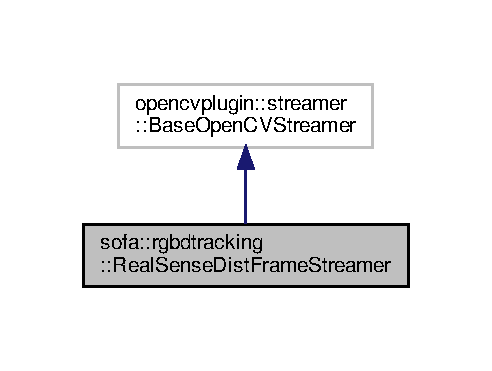
\includegraphics[width=236pt]{classsofa_1_1rgbdtracking_1_1_real_sense_dist_frame_streamer__inherit__graph}
\end{center}
\end{figure}


Collaboration diagram for sofa\+:\+:rgbdtracking\+:\+:Real\+Sense\+Dist\+Frame\+Streamer\+:\nopagebreak
\begin{figure}[H]
\begin{center}
\leavevmode
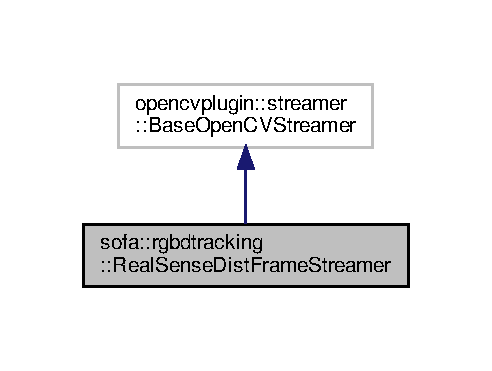
\includegraphics[width=236pt]{classsofa_1_1rgbdtracking_1_1_real_sense_dist_frame_streamer__coll__graph}
\end{center}
\end{figure}
\subsection*{Public Types}
\begin{DoxyCompactItemize}
\item 
\mbox{\Hypertarget{classsofa_1_1rgbdtracking_1_1_real_sense_dist_frame_streamer_afa7e78c7718a4c9284e392e8b5ef8a0a}\label{classsofa_1_1rgbdtracking_1_1_real_sense_dist_frame_streamer_afa7e78c7718a4c9284e392e8b5ef8a0a}} 
typedef opencvplugin\+::streamer\+::\+Base\+Open\+C\+V\+Streamer {\bfseries Inherited}
\end{DoxyCompactItemize}
\subsection*{Public Member Functions}
\begin{DoxyCompactItemize}
\item 
\mbox{\Hypertarget{classsofa_1_1rgbdtracking_1_1_real_sense_dist_frame_streamer_af6c388f58476267cf55047f977ba3b39}\label{classsofa_1_1rgbdtracking_1_1_real_sense_dist_frame_streamer_af6c388f58476267cf55047f977ba3b39}} 
{\bfseries S\+O\+F\+A\+\_\+\+C\+L\+A\+SS} (\hyperlink{classsofa_1_1rgbdtracking_1_1_real_sense_dist_frame_streamer}{Real\+Sense\+Dist\+Frame\+Streamer}, opencvplugin\+::streamer\+::\+Base\+Open\+C\+V\+Streamer)
\item 
\mbox{\Hypertarget{classsofa_1_1rgbdtracking_1_1_real_sense_dist_frame_streamer_acf9a105d197775cc56c840dce6edfb31}\label{classsofa_1_1rgbdtracking_1_1_real_sense_dist_frame_streamer_acf9a105d197775cc56c840dce6edfb31}} 
virtual void {\bfseries decode\+Image} (cv\+::\+Mat \&)
\item 
\mbox{\Hypertarget{classsofa_1_1rgbdtracking_1_1_real_sense_dist_frame_streamer_a0d02debb133e08b79d32eecb56969ab4}\label{classsofa_1_1rgbdtracking_1_1_real_sense_dist_frame_streamer_a0d02debb133e08b79d32eecb56969ab4}} 
void {\bfseries update\+File\+Stream} ()
\item 
\mbox{\Hypertarget{classsofa_1_1rgbdtracking_1_1_real_sense_dist_frame_streamer_a01d82d0618162c79579ef1ddeec97872}\label{classsofa_1_1rgbdtracking_1_1_real_sense_dist_frame_streamer_a01d82d0618162c79579ef1ddeec97872}} 
void {\bfseries read\+Frame} ()
\end{DoxyCompactItemize}
\subsection*{Public Attributes}
\begin{DoxyCompactItemize}
\item 
\mbox{\Hypertarget{classsofa_1_1rgbdtracking_1_1_real_sense_dist_frame_streamer_a66a7c3a880c2114197e3c476c5bbfbed}\label{classsofa_1_1rgbdtracking_1_1_real_sense_dist_frame_streamer_a66a7c3a880c2114197e3c476c5bbfbed}} 
Data$<$ std\+::string $>$ {\bfseries d\+\_\+filename}
\item 
\mbox{\Hypertarget{classsofa_1_1rgbdtracking_1_1_real_sense_dist_frame_streamer_acab30219890af914a1a0d200a9af16a5}\label{classsofa_1_1rgbdtracking_1_1_real_sense_dist_frame_streamer_acab30219890af914a1a0d200a9af16a5}} 
Data$<$ \hyperlink{classsofa_1_1rgbdtracking_1_1_real_sense_dist_frame}{Real\+Sense\+Dist\+Frame} $>$ {\bfseries d\+\_\+distframe}
\item 
\mbox{\Hypertarget{classsofa_1_1rgbdtracking_1_1_real_sense_dist_frame_streamer_ad5d699dd44589bb16c5560fb1bdbb661}\label{classsofa_1_1rgbdtracking_1_1_real_sense_dist_frame_streamer_ad5d699dd44589bb16c5560fb1bdbb661}} 
Data\+Callback {\bfseries c\+\_\+filename}
\item 
\mbox{\Hypertarget{classsofa_1_1rgbdtracking_1_1_real_sense_dist_frame_streamer_a6a62882f02e60b44fc462dd7bdd893ea}\label{classsofa_1_1rgbdtracking_1_1_real_sense_dist_frame_streamer_a6a62882f02e60b44fc462dd7bdd893ea}} 
std\+::\+F\+I\+LE $\ast$ {\bfseries filestream}
\end{DoxyCompactItemize}


\subsection{Detailed Description}
The \hyperlink{classsofa_1_1rgbdtracking_1_1_real_sense_dist_frame_streamer}{Real\+Sense\+Dist\+Frame\+Streamer} class Streams through distance frames in a file Implements Base\+Open\+C\+V\+Streamer. 

The documentation for this class was generated from the following file\+:\begin{DoxyCompactItemize}
\item 
src/sofa/realsenseplugin/projector/Real\+Sense\+Dist\+Frame.\+h\end{DoxyCompactItemize}

\hypertarget{structsofa_1_1rgbdtracking_1_1_real_sense_dist_frame_1_1_real_sense_dist_struct}{}\section{sofa\+:\+:rgbdtracking\+:\+:Real\+Sense\+Dist\+Frame\+:\+:Real\+Sense\+Dist\+Struct Struct Reference}
\label{structsofa_1_1rgbdtracking_1_1_real_sense_dist_frame_1_1_real_sense_dist_struct}\index{sofa\+::rgbdtracking\+::\+Real\+Sense\+Dist\+Frame\+::\+Real\+Sense\+Dist\+Struct@{sofa\+::rgbdtracking\+::\+Real\+Sense\+Dist\+Frame\+::\+Real\+Sense\+Dist\+Struct}}
\subsection*{Public Attributes}
\begin{DoxyCompactItemize}
\item 
\mbox{\Hypertarget{structsofa_1_1rgbdtracking_1_1_real_sense_dist_frame_1_1_real_sense_dist_struct_a9aebe63c9f0144dbc95337cc09c2266f}\label{structsofa_1_1rgbdtracking_1_1_real_sense_dist_frame_1_1_real_sense_dist_struct_a9aebe63c9f0144dbc95337cc09c2266f}} 
size\+\_\+t {\bfseries \+\_\+width}
\item 
\mbox{\Hypertarget{structsofa_1_1rgbdtracking_1_1_real_sense_dist_frame_1_1_real_sense_dist_struct_a7f08a343322668464a50912a970e1246}\label{structsofa_1_1rgbdtracking_1_1_real_sense_dist_frame_1_1_real_sense_dist_struct_a7f08a343322668464a50912a970e1246}} 
size\+\_\+t {\bfseries \+\_\+height}
\item 
\mbox{\Hypertarget{structsofa_1_1rgbdtracking_1_1_real_sense_dist_frame_1_1_real_sense_dist_struct_a8223b01562f5990926d5ebe4f449e5b6}\label{structsofa_1_1rgbdtracking_1_1_real_sense_dist_frame_1_1_real_sense_dist_struct_a8223b01562f5990926d5ebe4f449e5b6}} 
float $\ast$ {\bfseries frame}
\end{DoxyCompactItemize}


The documentation for this struct was generated from the following file\+:\begin{DoxyCompactItemize}
\item 
src/sofa/realsenseplugin/projector/Real\+Sense\+Dist\+Frame.\+h\end{DoxyCompactItemize}

\hypertarget{classsofa_1_1rgbdtracking_1_1_real_sense_grab_cut}{}\section{sofa\+:\+:rgbdtracking\+:\+:Real\+Sense\+Grab\+Cut Class Reference}
\label{classsofa_1_1rgbdtracking_1_1_real_sense_grab_cut}\index{sofa\+::rgbdtracking\+::\+Real\+Sense\+Grab\+Cut@{sofa\+::rgbdtracking\+::\+Real\+Sense\+Grab\+Cut}}


{\ttfamily \#include $<$Real\+Sense\+Grab\+Cut.\+h$>$}



Inheritance diagram for sofa\+:\+:rgbdtracking\+:\+:Real\+Sense\+Grab\+Cut\+:\nopagebreak
\begin{figure}[H]
\begin{center}
\leavevmode
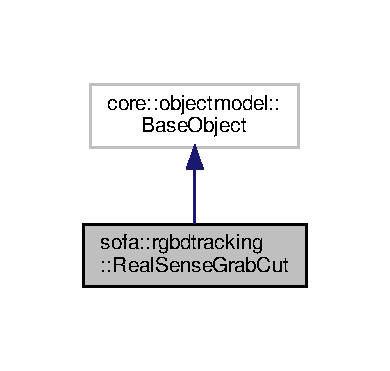
\includegraphics[width=187pt]{classsofa_1_1rgbdtracking_1_1_real_sense_grab_cut__inherit__graph}
\end{center}
\end{figure}


Collaboration diagram for sofa\+:\+:rgbdtracking\+:\+:Real\+Sense\+Grab\+Cut\+:\nopagebreak
\begin{figure}[H]
\begin{center}
\leavevmode
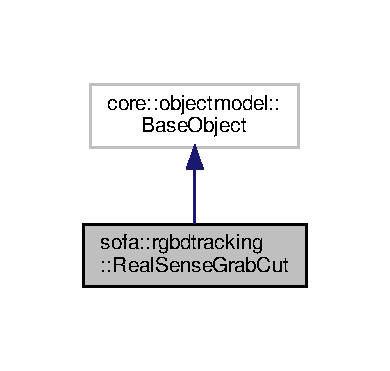
\includegraphics[width=187pt]{classsofa_1_1rgbdtracking_1_1_real_sense_grab_cut__coll__graph}
\end{center}
\end{figure}
\subsection*{Public Types}
\begin{DoxyCompactItemize}
\item 
typedef core\+::objectmodel\+::\+Base\+Object \hyperlink{classsofa_1_1rgbdtracking_1_1_real_sense_grab_cut_a3d3643071d86257ce05bd3e86a603763}{Inherited}
\end{DoxyCompactItemize}
\subsection*{Public Member Functions}
\begin{DoxyCompactItemize}
\item 
\hyperlink{classsofa_1_1rgbdtracking_1_1_real_sense_grab_cut_ab15c9f5be96ddd1ab0aefdab7701ad2b}{S\+O\+F\+A\+\_\+\+C\+L\+A\+SS} (\hyperlink{classsofa_1_1rgbdtracking_1_1_real_sense_grab_cut}{Real\+Sense\+Grab\+Cut}, core\+::objectmodel\+::\+Base\+Object)
\item 
\hyperlink{classsofa_1_1rgbdtracking_1_1_real_sense_grab_cut_ac99b63b2f756c9ac8073032d78ef334e}{Real\+Sense\+Grab\+Cut} ()
\item 
void \hyperlink{classsofa_1_1rgbdtracking_1_1_real_sense_grab_cut_a07ca12538fc84db6c54dfb9d4302a66b}{init} ()
\item 
void \hyperlink{classsofa_1_1rgbdtracking_1_1_real_sense_grab_cut_abd67d6e789b641b9ca90ad9b221b8ad4}{realsense\+\_\+grabcut} ()
\end{DoxyCompactItemize}
\subsection*{Public Attributes}
\begin{DoxyCompactItemize}
\item 
core\+::objectmodel\+::\+Single\+Link$<$ \hyperlink{classsofa_1_1rgbdtracking_1_1_real_sense_grab_cut}{Real\+Sense\+Grab\+Cut}, \hyperlink{classsofa_1_1rgbdtracking_1_1_real_sense_cam}{Real\+Sense\+Cam}, Base\+Link\+::\+F\+L\+A\+G\+\_\+\+S\+T\+O\+R\+E\+P\+A\+TH$\vert$Base\+Link\+::\+F\+L\+A\+G\+\_\+\+S\+T\+R\+O\+N\+G\+L\+I\+NK $>$ \hyperlink{classsofa_1_1rgbdtracking_1_1_real_sense_grab_cut_a761ad9c4afbcf2296b04a4431a294616}{l\+\_\+rs\+\_\+cam}
\item 
Data$<$ opencvplugin\+::\+Image\+Data $>$ \hyperlink{classsofa_1_1rgbdtracking_1_1_real_sense_grab_cut_a01f768822f64914b92234b03bd5c9d6f}{d\+\_\+image\+\_\+in}
\item 
Data$<$ opencvplugin\+::\+Image\+Data $>$ \hyperlink{classsofa_1_1rgbdtracking_1_1_real_sense_grab_cut_a2b2daf39abe1d4acf77316a41ada7ac8}{d\+\_\+image\+\_\+out}
\item 
Data$<$ opencvplugin\+::\+Image\+Data $>$ \hyperlink{classsofa_1_1rgbdtracking_1_1_real_sense_grab_cut_adeb52bee3090e991650f8a49b4bec7bd}{d\+\_\+depth\+\_\+in}
\item 
Data$<$ opencvplugin\+::\+Image\+Data $>$ \hyperlink{classsofa_1_1rgbdtracking_1_1_real_sense_grab_cut_a368ca4797dd54ff927e75d9cfc561787}{d\+\_\+depth\+\_\+out}
\item 
Data$<$ int $>$ \hyperlink{classsofa_1_1rgbdtracking_1_1_real_sense_grab_cut_af51a13c31b7b6a22f9e8e5b6f276870a}{d\+\_\+near\+\_\+thr}
\item 
Data$<$ int $>$ \hyperlink{classsofa_1_1rgbdtracking_1_1_real_sense_grab_cut_a8150b5cacf4c223b35a98bb6c78b3b5b}{d\+\_\+far\+\_\+thr}
\item 
Data$<$ defaulttype\+::\+Vec4i $>$ \hyperlink{classsofa_1_1rgbdtracking_1_1_real_sense_grab_cut_a1de3d863a69e379fbfe79756db8ad67c}{d\+\_\+rectangle}
\item 
\hyperlink{namespacesofa_1_1rgbdtracking_a00834a9204a667746fef9a402ccbfb55}{Data\+Callback} \hyperlink{classsofa_1_1rgbdtracking_1_1_real_sense_grab_cut_a5c45fc7332469e7272a01924f8db53cf}{c\+\_\+image\+\_\+in}
\item 
cv\+::\+Rect \hyperlink{classsofa_1_1rgbdtracking_1_1_real_sense_grab_cut_adc07cdbc1f27d1e1d1f189a722b6c99d}{rect}
\end{DoxyCompactItemize}
\subsection*{Protected Member Functions}
\begin{DoxyCompactItemize}
\item 
void \hyperlink{classsofa_1_1rgbdtracking_1_1_real_sense_grab_cut_abfa9d9858f8cf1ab78e9e908709383ec}{create\+\_\+mask\+\_\+from\+\_\+depth} (cv\+::\+Mat \&depth, int thresh, cv\+::\+Threshold\+Types type)
\end{DoxyCompactItemize}


\subsection{Detailed Description}
/!\textbackslash{} See \href{https://github.com/IntelRealSense/librealsense/blob/master/wrappers/opencv/grabcuts/rs-grabcuts.cpp}{\tt https\+://github.\+com/\+Intel\+Real\+Sense/librealsense/blob/master/wrappers/opencv/grabcuts/rs-\/grabcuts.\+cpp} for implementation details 

\subsection{Member Typedef Documentation}
\mbox{\Hypertarget{classsofa_1_1rgbdtracking_1_1_real_sense_grab_cut_a3d3643071d86257ce05bd3e86a603763}\label{classsofa_1_1rgbdtracking_1_1_real_sense_grab_cut_a3d3643071d86257ce05bd3e86a603763}} 
\index{sofa\+::rgbdtracking\+::\+Real\+Sense\+Grab\+Cut@{sofa\+::rgbdtracking\+::\+Real\+Sense\+Grab\+Cut}!Inherited@{Inherited}}
\index{Inherited@{Inherited}!sofa\+::rgbdtracking\+::\+Real\+Sense\+Grab\+Cut@{sofa\+::rgbdtracking\+::\+Real\+Sense\+Grab\+Cut}}
\subsubsection{\texorpdfstring{Inherited}{Inherited}}
{\footnotesize\ttfamily typedef core\+::objectmodel\+::\+Base\+Object \hyperlink{classsofa_1_1rgbdtracking_1_1_real_sense_grab_cut_a3d3643071d86257ce05bd3e86a603763}{sofa\+::rgbdtracking\+::\+Real\+Sense\+Grab\+Cut\+::\+Inherited}}



\subsection{Constructor \& Destructor Documentation}
\mbox{\Hypertarget{classsofa_1_1rgbdtracking_1_1_real_sense_grab_cut_ac99b63b2f756c9ac8073032d78ef334e}\label{classsofa_1_1rgbdtracking_1_1_real_sense_grab_cut_ac99b63b2f756c9ac8073032d78ef334e}} 
\index{sofa\+::rgbdtracking\+::\+Real\+Sense\+Grab\+Cut@{sofa\+::rgbdtracking\+::\+Real\+Sense\+Grab\+Cut}!Real\+Sense\+Grab\+Cut@{Real\+Sense\+Grab\+Cut}}
\index{Real\+Sense\+Grab\+Cut@{Real\+Sense\+Grab\+Cut}!sofa\+::rgbdtracking\+::\+Real\+Sense\+Grab\+Cut@{sofa\+::rgbdtracking\+::\+Real\+Sense\+Grab\+Cut}}
\subsubsection{\texorpdfstring{Real\+Sense\+Grab\+Cut()}{RealSenseGrabCut()}}
{\footnotesize\ttfamily sofa\+::rgbdtracking\+::\+Real\+Sense\+Grab\+Cut\+::\+Real\+Sense\+Grab\+Cut (\begin{DoxyParamCaption}{ }\end{DoxyParamCaption})\hspace{0.3cm}{\ttfamily [inline]}}



\subsection{Member Function Documentation}
\mbox{\Hypertarget{classsofa_1_1rgbdtracking_1_1_real_sense_grab_cut_abfa9d9858f8cf1ab78e9e908709383ec}\label{classsofa_1_1rgbdtracking_1_1_real_sense_grab_cut_abfa9d9858f8cf1ab78e9e908709383ec}} 
\index{sofa\+::rgbdtracking\+::\+Real\+Sense\+Grab\+Cut@{sofa\+::rgbdtracking\+::\+Real\+Sense\+Grab\+Cut}!create\+\_\+mask\+\_\+from\+\_\+depth@{create\+\_\+mask\+\_\+from\+\_\+depth}}
\index{create\+\_\+mask\+\_\+from\+\_\+depth@{create\+\_\+mask\+\_\+from\+\_\+depth}!sofa\+::rgbdtracking\+::\+Real\+Sense\+Grab\+Cut@{sofa\+::rgbdtracking\+::\+Real\+Sense\+Grab\+Cut}}
\subsubsection{\texorpdfstring{create\+\_\+mask\+\_\+from\+\_\+depth()}{create\_mask\_from\_depth()}}
{\footnotesize\ttfamily void sofa\+::rgbdtracking\+::\+Real\+Sense\+Grab\+Cut\+::create\+\_\+mask\+\_\+from\+\_\+depth (\begin{DoxyParamCaption}\item[{cv\+::\+Mat \&}]{depth,  }\item[{int}]{thresh,  }\item[{cv\+::\+Threshold\+Types}]{type }\end{DoxyParamCaption})\hspace{0.3cm}{\ttfamily [inline]}, {\ttfamily [protected]}}

\mbox{\Hypertarget{classsofa_1_1rgbdtracking_1_1_real_sense_grab_cut_a07ca12538fc84db6c54dfb9d4302a66b}\label{classsofa_1_1rgbdtracking_1_1_real_sense_grab_cut_a07ca12538fc84db6c54dfb9d4302a66b}} 
\index{sofa\+::rgbdtracking\+::\+Real\+Sense\+Grab\+Cut@{sofa\+::rgbdtracking\+::\+Real\+Sense\+Grab\+Cut}!init@{init}}
\index{init@{init}!sofa\+::rgbdtracking\+::\+Real\+Sense\+Grab\+Cut@{sofa\+::rgbdtracking\+::\+Real\+Sense\+Grab\+Cut}}
\subsubsection{\texorpdfstring{init()}{init()}}
{\footnotesize\ttfamily void sofa\+::rgbdtracking\+::\+Real\+Sense\+Grab\+Cut\+::init (\begin{DoxyParamCaption}{ }\end{DoxyParamCaption})\hspace{0.3cm}{\ttfamily [inline]}}

\mbox{\Hypertarget{classsofa_1_1rgbdtracking_1_1_real_sense_grab_cut_abd67d6e789b641b9ca90ad9b221b8ad4}\label{classsofa_1_1rgbdtracking_1_1_real_sense_grab_cut_abd67d6e789b641b9ca90ad9b221b8ad4}} 
\index{sofa\+::rgbdtracking\+::\+Real\+Sense\+Grab\+Cut@{sofa\+::rgbdtracking\+::\+Real\+Sense\+Grab\+Cut}!realsense\+\_\+grabcut@{realsense\+\_\+grabcut}}
\index{realsense\+\_\+grabcut@{realsense\+\_\+grabcut}!sofa\+::rgbdtracking\+::\+Real\+Sense\+Grab\+Cut@{sofa\+::rgbdtracking\+::\+Real\+Sense\+Grab\+Cut}}
\subsubsection{\texorpdfstring{realsense\+\_\+grabcut()}{realsense\_grabcut()}}
{\footnotesize\ttfamily void sofa\+::rgbdtracking\+::\+Real\+Sense\+Grab\+Cut\+::realsense\+\_\+grabcut (\begin{DoxyParamCaption}{ }\end{DoxyParamCaption})\hspace{0.3cm}{\ttfamily [inline]}}

\mbox{\Hypertarget{classsofa_1_1rgbdtracking_1_1_real_sense_grab_cut_ab15c9f5be96ddd1ab0aefdab7701ad2b}\label{classsofa_1_1rgbdtracking_1_1_real_sense_grab_cut_ab15c9f5be96ddd1ab0aefdab7701ad2b}} 
\index{sofa\+::rgbdtracking\+::\+Real\+Sense\+Grab\+Cut@{sofa\+::rgbdtracking\+::\+Real\+Sense\+Grab\+Cut}!S\+O\+F\+A\+\_\+\+C\+L\+A\+SS@{S\+O\+F\+A\+\_\+\+C\+L\+A\+SS}}
\index{S\+O\+F\+A\+\_\+\+C\+L\+A\+SS@{S\+O\+F\+A\+\_\+\+C\+L\+A\+SS}!sofa\+::rgbdtracking\+::\+Real\+Sense\+Grab\+Cut@{sofa\+::rgbdtracking\+::\+Real\+Sense\+Grab\+Cut}}
\subsubsection{\texorpdfstring{S\+O\+F\+A\+\_\+\+C\+L\+A\+S\+S()}{SOFA\_CLASS()}}
{\footnotesize\ttfamily sofa\+::rgbdtracking\+::\+Real\+Sense\+Grab\+Cut\+::\+S\+O\+F\+A\+\_\+\+C\+L\+A\+SS (\begin{DoxyParamCaption}\item[{\hyperlink{classsofa_1_1rgbdtracking_1_1_real_sense_grab_cut}{Real\+Sense\+Grab\+Cut}}]{,  }\item[{core\+::objectmodel\+::\+Base\+Object}]{ }\end{DoxyParamCaption})}



\subsection{Member Data Documentation}
\mbox{\Hypertarget{classsofa_1_1rgbdtracking_1_1_real_sense_grab_cut_a5c45fc7332469e7272a01924f8db53cf}\label{classsofa_1_1rgbdtracking_1_1_real_sense_grab_cut_a5c45fc7332469e7272a01924f8db53cf}} 
\index{sofa\+::rgbdtracking\+::\+Real\+Sense\+Grab\+Cut@{sofa\+::rgbdtracking\+::\+Real\+Sense\+Grab\+Cut}!c\+\_\+image\+\_\+in@{c\+\_\+image\+\_\+in}}
\index{c\+\_\+image\+\_\+in@{c\+\_\+image\+\_\+in}!sofa\+::rgbdtracking\+::\+Real\+Sense\+Grab\+Cut@{sofa\+::rgbdtracking\+::\+Real\+Sense\+Grab\+Cut}}
\subsubsection{\texorpdfstring{c\+\_\+image\+\_\+in}{c\_image\_in}}
{\footnotesize\ttfamily \hyperlink{namespacesofa_1_1rgbdtracking_a00834a9204a667746fef9a402ccbfb55}{Data\+Callback} sofa\+::rgbdtracking\+::\+Real\+Sense\+Grab\+Cut\+::c\+\_\+image\+\_\+in}

\mbox{\Hypertarget{classsofa_1_1rgbdtracking_1_1_real_sense_grab_cut_adeb52bee3090e991650f8a49b4bec7bd}\label{classsofa_1_1rgbdtracking_1_1_real_sense_grab_cut_adeb52bee3090e991650f8a49b4bec7bd}} 
\index{sofa\+::rgbdtracking\+::\+Real\+Sense\+Grab\+Cut@{sofa\+::rgbdtracking\+::\+Real\+Sense\+Grab\+Cut}!d\+\_\+depth\+\_\+in@{d\+\_\+depth\+\_\+in}}
\index{d\+\_\+depth\+\_\+in@{d\+\_\+depth\+\_\+in}!sofa\+::rgbdtracking\+::\+Real\+Sense\+Grab\+Cut@{sofa\+::rgbdtracking\+::\+Real\+Sense\+Grab\+Cut}}
\subsubsection{\texorpdfstring{d\+\_\+depth\+\_\+in}{d\_depth\_in}}
{\footnotesize\ttfamily Data$<$opencvplugin\+::\+Image\+Data$>$ sofa\+::rgbdtracking\+::\+Real\+Sense\+Grab\+Cut\+::d\+\_\+depth\+\_\+in}

\mbox{\Hypertarget{classsofa_1_1rgbdtracking_1_1_real_sense_grab_cut_a368ca4797dd54ff927e75d9cfc561787}\label{classsofa_1_1rgbdtracking_1_1_real_sense_grab_cut_a368ca4797dd54ff927e75d9cfc561787}} 
\index{sofa\+::rgbdtracking\+::\+Real\+Sense\+Grab\+Cut@{sofa\+::rgbdtracking\+::\+Real\+Sense\+Grab\+Cut}!d\+\_\+depth\+\_\+out@{d\+\_\+depth\+\_\+out}}
\index{d\+\_\+depth\+\_\+out@{d\+\_\+depth\+\_\+out}!sofa\+::rgbdtracking\+::\+Real\+Sense\+Grab\+Cut@{sofa\+::rgbdtracking\+::\+Real\+Sense\+Grab\+Cut}}
\subsubsection{\texorpdfstring{d\+\_\+depth\+\_\+out}{d\_depth\_out}}
{\footnotesize\ttfamily Data$<$opencvplugin\+::\+Image\+Data$>$ sofa\+::rgbdtracking\+::\+Real\+Sense\+Grab\+Cut\+::d\+\_\+depth\+\_\+out}

\mbox{\Hypertarget{classsofa_1_1rgbdtracking_1_1_real_sense_grab_cut_a8150b5cacf4c223b35a98bb6c78b3b5b}\label{classsofa_1_1rgbdtracking_1_1_real_sense_grab_cut_a8150b5cacf4c223b35a98bb6c78b3b5b}} 
\index{sofa\+::rgbdtracking\+::\+Real\+Sense\+Grab\+Cut@{sofa\+::rgbdtracking\+::\+Real\+Sense\+Grab\+Cut}!d\+\_\+far\+\_\+thr@{d\+\_\+far\+\_\+thr}}
\index{d\+\_\+far\+\_\+thr@{d\+\_\+far\+\_\+thr}!sofa\+::rgbdtracking\+::\+Real\+Sense\+Grab\+Cut@{sofa\+::rgbdtracking\+::\+Real\+Sense\+Grab\+Cut}}
\subsubsection{\texorpdfstring{d\+\_\+far\+\_\+thr}{d\_far\_thr}}
{\footnotesize\ttfamily Data$<$int$>$ sofa\+::rgbdtracking\+::\+Real\+Sense\+Grab\+Cut\+::d\+\_\+far\+\_\+thr}

\mbox{\Hypertarget{classsofa_1_1rgbdtracking_1_1_real_sense_grab_cut_a01f768822f64914b92234b03bd5c9d6f}\label{classsofa_1_1rgbdtracking_1_1_real_sense_grab_cut_a01f768822f64914b92234b03bd5c9d6f}} 
\index{sofa\+::rgbdtracking\+::\+Real\+Sense\+Grab\+Cut@{sofa\+::rgbdtracking\+::\+Real\+Sense\+Grab\+Cut}!d\+\_\+image\+\_\+in@{d\+\_\+image\+\_\+in}}
\index{d\+\_\+image\+\_\+in@{d\+\_\+image\+\_\+in}!sofa\+::rgbdtracking\+::\+Real\+Sense\+Grab\+Cut@{sofa\+::rgbdtracking\+::\+Real\+Sense\+Grab\+Cut}}
\subsubsection{\texorpdfstring{d\+\_\+image\+\_\+in}{d\_image\_in}}
{\footnotesize\ttfamily Data$<$opencvplugin\+::\+Image\+Data$>$ sofa\+::rgbdtracking\+::\+Real\+Sense\+Grab\+Cut\+::d\+\_\+image\+\_\+in}

\mbox{\Hypertarget{classsofa_1_1rgbdtracking_1_1_real_sense_grab_cut_a2b2daf39abe1d4acf77316a41ada7ac8}\label{classsofa_1_1rgbdtracking_1_1_real_sense_grab_cut_a2b2daf39abe1d4acf77316a41ada7ac8}} 
\index{sofa\+::rgbdtracking\+::\+Real\+Sense\+Grab\+Cut@{sofa\+::rgbdtracking\+::\+Real\+Sense\+Grab\+Cut}!d\+\_\+image\+\_\+out@{d\+\_\+image\+\_\+out}}
\index{d\+\_\+image\+\_\+out@{d\+\_\+image\+\_\+out}!sofa\+::rgbdtracking\+::\+Real\+Sense\+Grab\+Cut@{sofa\+::rgbdtracking\+::\+Real\+Sense\+Grab\+Cut}}
\subsubsection{\texorpdfstring{d\+\_\+image\+\_\+out}{d\_image\_out}}
{\footnotesize\ttfamily Data$<$opencvplugin\+::\+Image\+Data$>$ sofa\+::rgbdtracking\+::\+Real\+Sense\+Grab\+Cut\+::d\+\_\+image\+\_\+out}

\mbox{\Hypertarget{classsofa_1_1rgbdtracking_1_1_real_sense_grab_cut_af51a13c31b7b6a22f9e8e5b6f276870a}\label{classsofa_1_1rgbdtracking_1_1_real_sense_grab_cut_af51a13c31b7b6a22f9e8e5b6f276870a}} 
\index{sofa\+::rgbdtracking\+::\+Real\+Sense\+Grab\+Cut@{sofa\+::rgbdtracking\+::\+Real\+Sense\+Grab\+Cut}!d\+\_\+near\+\_\+thr@{d\+\_\+near\+\_\+thr}}
\index{d\+\_\+near\+\_\+thr@{d\+\_\+near\+\_\+thr}!sofa\+::rgbdtracking\+::\+Real\+Sense\+Grab\+Cut@{sofa\+::rgbdtracking\+::\+Real\+Sense\+Grab\+Cut}}
\subsubsection{\texorpdfstring{d\+\_\+near\+\_\+thr}{d\_near\_thr}}
{\footnotesize\ttfamily Data$<$int$>$ sofa\+::rgbdtracking\+::\+Real\+Sense\+Grab\+Cut\+::d\+\_\+near\+\_\+thr}

\mbox{\Hypertarget{classsofa_1_1rgbdtracking_1_1_real_sense_grab_cut_a1de3d863a69e379fbfe79756db8ad67c}\label{classsofa_1_1rgbdtracking_1_1_real_sense_grab_cut_a1de3d863a69e379fbfe79756db8ad67c}} 
\index{sofa\+::rgbdtracking\+::\+Real\+Sense\+Grab\+Cut@{sofa\+::rgbdtracking\+::\+Real\+Sense\+Grab\+Cut}!d\+\_\+rectangle@{d\+\_\+rectangle}}
\index{d\+\_\+rectangle@{d\+\_\+rectangle}!sofa\+::rgbdtracking\+::\+Real\+Sense\+Grab\+Cut@{sofa\+::rgbdtracking\+::\+Real\+Sense\+Grab\+Cut}}
\subsubsection{\texorpdfstring{d\+\_\+rectangle}{d\_rectangle}}
{\footnotesize\ttfamily Data$<$defaulttype\+::\+Vec4i$>$ sofa\+::rgbdtracking\+::\+Real\+Sense\+Grab\+Cut\+::d\+\_\+rectangle}

\mbox{\Hypertarget{classsofa_1_1rgbdtracking_1_1_real_sense_grab_cut_a761ad9c4afbcf2296b04a4431a294616}\label{classsofa_1_1rgbdtracking_1_1_real_sense_grab_cut_a761ad9c4afbcf2296b04a4431a294616}} 
\index{sofa\+::rgbdtracking\+::\+Real\+Sense\+Grab\+Cut@{sofa\+::rgbdtracking\+::\+Real\+Sense\+Grab\+Cut}!l\+\_\+rs\+\_\+cam@{l\+\_\+rs\+\_\+cam}}
\index{l\+\_\+rs\+\_\+cam@{l\+\_\+rs\+\_\+cam}!sofa\+::rgbdtracking\+::\+Real\+Sense\+Grab\+Cut@{sofa\+::rgbdtracking\+::\+Real\+Sense\+Grab\+Cut}}
\subsubsection{\texorpdfstring{l\+\_\+rs\+\_\+cam}{l\_rs\_cam}}
{\footnotesize\ttfamily core\+::objectmodel\+::\+Single\+Link$<$ \hyperlink{classsofa_1_1rgbdtracking_1_1_real_sense_grab_cut}{Real\+Sense\+Grab\+Cut}, \hyperlink{classsofa_1_1rgbdtracking_1_1_real_sense_cam}{Real\+Sense\+Cam}, Base\+Link\+::\+F\+L\+A\+G\+\_\+\+S\+T\+O\+R\+E\+P\+A\+TH$\vert$Base\+Link\+::\+F\+L\+A\+G\+\_\+\+S\+T\+R\+O\+N\+G\+L\+I\+NK $>$ sofa\+::rgbdtracking\+::\+Real\+Sense\+Grab\+Cut\+::l\+\_\+rs\+\_\+cam}

\mbox{\Hypertarget{classsofa_1_1rgbdtracking_1_1_real_sense_grab_cut_adc07cdbc1f27d1e1d1f189a722b6c99d}\label{classsofa_1_1rgbdtracking_1_1_real_sense_grab_cut_adc07cdbc1f27d1e1d1f189a722b6c99d}} 
\index{sofa\+::rgbdtracking\+::\+Real\+Sense\+Grab\+Cut@{sofa\+::rgbdtracking\+::\+Real\+Sense\+Grab\+Cut}!rect@{rect}}
\index{rect@{rect}!sofa\+::rgbdtracking\+::\+Real\+Sense\+Grab\+Cut@{sofa\+::rgbdtracking\+::\+Real\+Sense\+Grab\+Cut}}
\subsubsection{\texorpdfstring{rect}{rect}}
{\footnotesize\ttfamily cv\+::\+Rect sofa\+::rgbdtracking\+::\+Real\+Sense\+Grab\+Cut\+::rect}



The documentation for this class was generated from the following file\+:\begin{DoxyCompactItemize}
\item 
src/sofa/realsenseplugin/utils/\hyperlink{_real_sense_grab_cut_8h}{Real\+Sense\+Grab\+Cut.\+h}\end{DoxyCompactItemize}

\hypertarget{classsofa_1_1rgbdtracking_1_1_real_sense_mask_deprojector}{}\section{sofa\+:\+:rgbdtracking\+:\+:Real\+Sense\+Mask\+Deprojector Class Reference}
\label{classsofa_1_1rgbdtracking_1_1_real_sense_mask_deprojector}\index{sofa\+::rgbdtracking\+::\+Real\+Sense\+Mask\+Deprojector@{sofa\+::rgbdtracking\+::\+Real\+Sense\+Mask\+Deprojector}}


The \hyperlink{classsofa_1_1rgbdtracking_1_1_real_sense_mask_deprojector}{Real\+Sense\+Mask\+Deprojector} class deprojects a set of points depending on a 2D binary mask defined as an image in d\+\_\+input (label input in sofa)  




{\ttfamily \#include $<$Real\+Sense\+Mask\+Deprojector.\+h$>$}



Inheritance diagram for sofa\+:\+:rgbdtracking\+:\+:Real\+Sense\+Mask\+Deprojector\+:\nopagebreak
\begin{figure}[H]
\begin{center}
\leavevmode
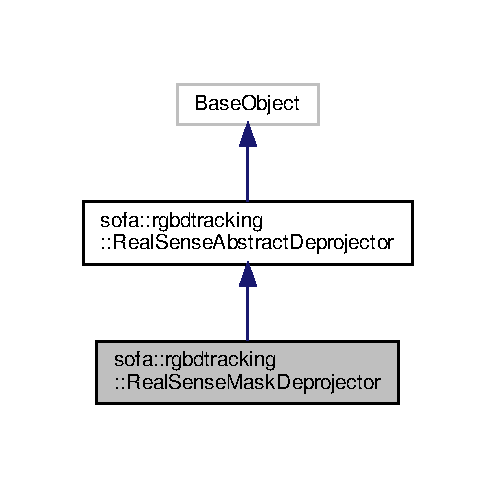
\includegraphics[width=238pt]{classsofa_1_1rgbdtracking_1_1_real_sense_mask_deprojector__inherit__graph}
\end{center}
\end{figure}


Collaboration diagram for sofa\+:\+:rgbdtracking\+:\+:Real\+Sense\+Mask\+Deprojector\+:\nopagebreak
\begin{figure}[H]
\begin{center}
\leavevmode
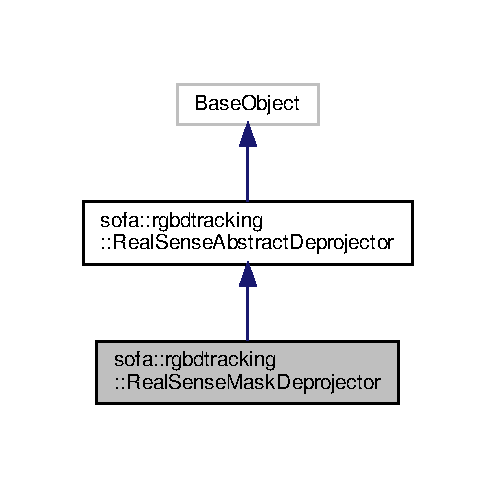
\includegraphics[width=238pt]{classsofa_1_1rgbdtracking_1_1_real_sense_mask_deprojector__coll__graph}
\end{center}
\end{figure}
\subsection*{Public Types}
\begin{DoxyCompactItemize}
\item 
\mbox{\Hypertarget{classsofa_1_1rgbdtracking_1_1_real_sense_mask_deprojector_aa8f05cf5049f6cef0ea54ba40efa0727}\label{classsofa_1_1rgbdtracking_1_1_real_sense_mask_deprojector_aa8f05cf5049f6cef0ea54ba40efa0727}} 
typedef \hyperlink{classsofa_1_1rgbdtracking_1_1_real_sense_abstract_deprojector}{Real\+Sense\+Abstract\+Deprojector} {\bfseries Inherited}
\end{DoxyCompactItemize}
\subsection*{Public Member Functions}
\begin{DoxyCompactItemize}
\item 
\mbox{\Hypertarget{classsofa_1_1rgbdtracking_1_1_real_sense_mask_deprojector_a7661938009502eb3591b1cf196b3489d}\label{classsofa_1_1rgbdtracking_1_1_real_sense_mask_deprojector_a7661938009502eb3591b1cf196b3489d}} 
{\bfseries S\+O\+F\+A\+\_\+\+C\+L\+A\+SS} (\hyperlink{classsofa_1_1rgbdtracking_1_1_real_sense_mask_deprojector}{Real\+Sense\+Mask\+Deprojector}, Inherited)
\end{DoxyCompactItemize}
\subsection*{Public Attributes}
\begin{DoxyCompactItemize}
\item 
\mbox{\Hypertarget{classsofa_1_1rgbdtracking_1_1_real_sense_mask_deprojector_ada97b307e34090d3fb987124a936459b}\label{classsofa_1_1rgbdtracking_1_1_real_sense_mask_deprojector_ada97b307e34090d3fb987124a936459b}} 
Data$<$ opencvplugin\+::\+Image\+Data $>$ \hyperlink{classsofa_1_1rgbdtracking_1_1_real_sense_mask_deprojector_ada97b307e34090d3fb987124a936459b}{d\+\_\+input}
\begin{DoxyCompactList}\small\item\em input binary mask for filtering reprojections \end{DoxyCompactList}\item 
\mbox{\Hypertarget{classsofa_1_1rgbdtracking_1_1_real_sense_mask_deprojector_a5ef4d4dff52a6f68a3153fbfb9599a4f}\label{classsofa_1_1rgbdtracking_1_1_real_sense_mask_deprojector_a5ef4d4dff52a6f68a3153fbfb9599a4f}} 
Data\+Callback {\bfseries c\+\_\+image}
\end{DoxyCompactItemize}


\subsection{Detailed Description}
The \hyperlink{classsofa_1_1rgbdtracking_1_1_real_sense_mask_deprojector}{Real\+Sense\+Mask\+Deprojector} class deprojects a set of points depending on a 2D binary mask defined as an image in d\+\_\+input (label input in sofa) 

The documentation for this class was generated from the following file\+:\begin{DoxyCompactItemize}
\item 
src/sofa/realsenseplugin/projector/Real\+Sense\+Mask\+Deprojector.\+h\end{DoxyCompactItemize}

\hypertarget{classsofa_1_1rgbdtracking_1_1_real_sense_multi_cam}{}\section{sofa\+:\+:rgbdtracking\+:\+:Real\+Sense\+Multi\+Cam Class Reference}
\label{classsofa_1_1rgbdtracking_1_1_real_sense_multi_cam}\index{sofa\+::rgbdtracking\+::\+Real\+Sense\+Multi\+Cam@{sofa\+::rgbdtracking\+::\+Real\+Sense\+Multi\+Cam}}


The \hyperlink{classsofa_1_1rgbdtracking_1_1_real_sense_multi_cam}{Real\+Sense\+Multi\+Cam} class tries listing all realsense cameras connected and instanciates Virtual\+Camera components accordingly.  




{\ttfamily \#include $<$Real\+Sense\+Multi\+Cam.\+h$>$}



Inheritance diagram for sofa\+:\+:rgbdtracking\+:\+:Real\+Sense\+Multi\+Cam\+:\nopagebreak
\begin{figure}[H]
\begin{center}
\leavevmode
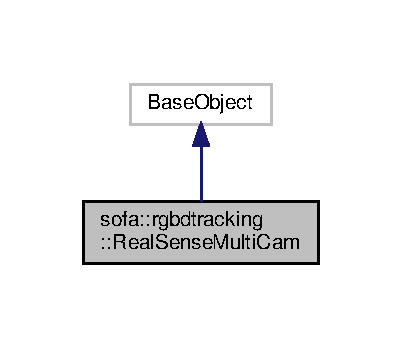
\includegraphics[width=193pt]{classsofa_1_1rgbdtracking_1_1_real_sense_multi_cam__inherit__graph}
\end{center}
\end{figure}


Collaboration diagram for sofa\+:\+:rgbdtracking\+:\+:Real\+Sense\+Multi\+Cam\+:\nopagebreak
\begin{figure}[H]
\begin{center}
\leavevmode
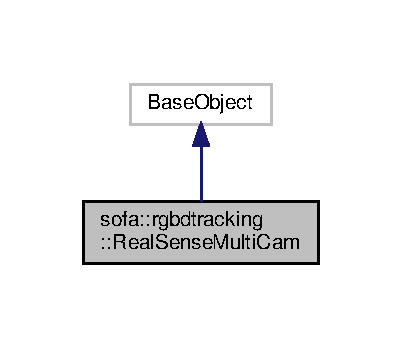
\includegraphics[width=193pt]{classsofa_1_1rgbdtracking_1_1_real_sense_multi_cam__coll__graph}
\end{center}
\end{figure}
\subsection*{Public Types}
\begin{DoxyCompactItemize}
\item 
typedef core\+::objectmodel\+::\+Base\+Object \hyperlink{classsofa_1_1rgbdtracking_1_1_real_sense_multi_cam_ac46918355916b1af92c7aabc7e244e39}{Inherited}
\end{DoxyCompactItemize}
\subsection*{Public Member Functions}
\begin{DoxyCompactItemize}
\item 
\hyperlink{classsofa_1_1rgbdtracking_1_1_real_sense_multi_cam_a580a759696c9de476a75c1aabc955669}{S\+O\+F\+A\+\_\+\+C\+L\+A\+SS} (\hyperlink{classsofa_1_1rgbdtracking_1_1_real_sense_multi_cam}{Real\+Sense\+Multi\+Cam}, \hyperlink{classsofa_1_1rgbdtracking_1_1_real_sense_multi_cam_ac46918355916b1af92c7aabc7e244e39}{Inherited})
\item 
\hyperlink{classsofa_1_1rgbdtracking_1_1_real_sense_multi_cam_a7f9c9f94849adee3e90212159b635396}{Real\+Sense\+Multi\+Cam} ()
\item 
std\+::vector$<$ std\+::string $>$ \hyperlink{classsofa_1_1rgbdtracking_1_1_real_sense_multi_cam_ae06084e54a01de953a441b1994ad22e7}{list\+Serial\+Num} ()
\item 
void \hyperlink{classsofa_1_1rgbdtracking_1_1_real_sense_multi_cam_ac93ba93ba4d82475f37e4300173b168d}{init} ()
\item 
void \hyperlink{classsofa_1_1rgbdtracking_1_1_real_sense_multi_cam_a1aea376ebf5a7ee03af4cae251380e89}{add\+\_\+realsense\+Cam} (core\+::objectmodel\+::\+Base\+Context\+::\+S\+Ptr node, std\+::string serial, size\+\_\+t i)
\end{DoxyCompactItemize}


\subsection{Detailed Description}
The \hyperlink{classsofa_1_1rgbdtracking_1_1_real_sense_multi_cam}{Real\+Sense\+Multi\+Cam} class tries listing all realsense cameras connected and instanciates Virtual\+Camera components accordingly. 

\subsection{Member Typedef Documentation}
\mbox{\Hypertarget{classsofa_1_1rgbdtracking_1_1_real_sense_multi_cam_ac46918355916b1af92c7aabc7e244e39}\label{classsofa_1_1rgbdtracking_1_1_real_sense_multi_cam_ac46918355916b1af92c7aabc7e244e39}} 
\index{sofa\+::rgbdtracking\+::\+Real\+Sense\+Multi\+Cam@{sofa\+::rgbdtracking\+::\+Real\+Sense\+Multi\+Cam}!Inherited@{Inherited}}
\index{Inherited@{Inherited}!sofa\+::rgbdtracking\+::\+Real\+Sense\+Multi\+Cam@{sofa\+::rgbdtracking\+::\+Real\+Sense\+Multi\+Cam}}
\subsubsection{\texorpdfstring{Inherited}{Inherited}}
{\footnotesize\ttfamily typedef core\+::objectmodel\+::\+Base\+Object \hyperlink{classsofa_1_1rgbdtracking_1_1_real_sense_multi_cam_ac46918355916b1af92c7aabc7e244e39}{sofa\+::rgbdtracking\+::\+Real\+Sense\+Multi\+Cam\+::\+Inherited}}



\subsection{Constructor \& Destructor Documentation}
\mbox{\Hypertarget{classsofa_1_1rgbdtracking_1_1_real_sense_multi_cam_a7f9c9f94849adee3e90212159b635396}\label{classsofa_1_1rgbdtracking_1_1_real_sense_multi_cam_a7f9c9f94849adee3e90212159b635396}} 
\index{sofa\+::rgbdtracking\+::\+Real\+Sense\+Multi\+Cam@{sofa\+::rgbdtracking\+::\+Real\+Sense\+Multi\+Cam}!Real\+Sense\+Multi\+Cam@{Real\+Sense\+Multi\+Cam}}
\index{Real\+Sense\+Multi\+Cam@{Real\+Sense\+Multi\+Cam}!sofa\+::rgbdtracking\+::\+Real\+Sense\+Multi\+Cam@{sofa\+::rgbdtracking\+::\+Real\+Sense\+Multi\+Cam}}
\subsubsection{\texorpdfstring{Real\+Sense\+Multi\+Cam()}{RealSenseMultiCam()}}
{\footnotesize\ttfamily sofa\+::rgbdtracking\+::\+Real\+Sense\+Multi\+Cam\+::\+Real\+Sense\+Multi\+Cam (\begin{DoxyParamCaption}{ }\end{DoxyParamCaption})\hspace{0.3cm}{\ttfamily [inline]}}



\subsection{Member Function Documentation}
\mbox{\Hypertarget{classsofa_1_1rgbdtracking_1_1_real_sense_multi_cam_a1aea376ebf5a7ee03af4cae251380e89}\label{classsofa_1_1rgbdtracking_1_1_real_sense_multi_cam_a1aea376ebf5a7ee03af4cae251380e89}} 
\index{sofa\+::rgbdtracking\+::\+Real\+Sense\+Multi\+Cam@{sofa\+::rgbdtracking\+::\+Real\+Sense\+Multi\+Cam}!add\+\_\+realsense\+Cam@{add\+\_\+realsense\+Cam}}
\index{add\+\_\+realsense\+Cam@{add\+\_\+realsense\+Cam}!sofa\+::rgbdtracking\+::\+Real\+Sense\+Multi\+Cam@{sofa\+::rgbdtracking\+::\+Real\+Sense\+Multi\+Cam}}
\subsubsection{\texorpdfstring{add\+\_\+realsense\+Cam()}{add\_realsenseCam()}}
{\footnotesize\ttfamily void sofa\+::rgbdtracking\+::\+Real\+Sense\+Multi\+Cam\+::add\+\_\+realsense\+Cam (\begin{DoxyParamCaption}\item[{core\+::objectmodel\+::\+Base\+Context\+::\+S\+Ptr}]{node,  }\item[{std\+::string}]{serial,  }\item[{size\+\_\+t}]{i }\end{DoxyParamCaption})\hspace{0.3cm}{\ttfamily [inline]}}

\mbox{\Hypertarget{classsofa_1_1rgbdtracking_1_1_real_sense_multi_cam_ac93ba93ba4d82475f37e4300173b168d}\label{classsofa_1_1rgbdtracking_1_1_real_sense_multi_cam_ac93ba93ba4d82475f37e4300173b168d}} 
\index{sofa\+::rgbdtracking\+::\+Real\+Sense\+Multi\+Cam@{sofa\+::rgbdtracking\+::\+Real\+Sense\+Multi\+Cam}!init@{init}}
\index{init@{init}!sofa\+::rgbdtracking\+::\+Real\+Sense\+Multi\+Cam@{sofa\+::rgbdtracking\+::\+Real\+Sense\+Multi\+Cam}}
\subsubsection{\texorpdfstring{init()}{init()}}
{\footnotesize\ttfamily void sofa\+::rgbdtracking\+::\+Real\+Sense\+Multi\+Cam\+::init (\begin{DoxyParamCaption}{ }\end{DoxyParamCaption})\hspace{0.3cm}{\ttfamily [inline]}}

\mbox{\Hypertarget{classsofa_1_1rgbdtracking_1_1_real_sense_multi_cam_ae06084e54a01de953a441b1994ad22e7}\label{classsofa_1_1rgbdtracking_1_1_real_sense_multi_cam_ae06084e54a01de953a441b1994ad22e7}} 
\index{sofa\+::rgbdtracking\+::\+Real\+Sense\+Multi\+Cam@{sofa\+::rgbdtracking\+::\+Real\+Sense\+Multi\+Cam}!list\+Serial\+Num@{list\+Serial\+Num}}
\index{list\+Serial\+Num@{list\+Serial\+Num}!sofa\+::rgbdtracking\+::\+Real\+Sense\+Multi\+Cam@{sofa\+::rgbdtracking\+::\+Real\+Sense\+Multi\+Cam}}
\subsubsection{\texorpdfstring{list\+Serial\+Num()}{listSerialNum()}}
{\footnotesize\ttfamily std\+::vector$<$std\+::string$>$ sofa\+::rgbdtracking\+::\+Real\+Sense\+Multi\+Cam\+::list\+Serial\+Num (\begin{DoxyParamCaption}{ }\end{DoxyParamCaption})\hspace{0.3cm}{\ttfamily [inline]}}

\mbox{\Hypertarget{classsofa_1_1rgbdtracking_1_1_real_sense_multi_cam_a580a759696c9de476a75c1aabc955669}\label{classsofa_1_1rgbdtracking_1_1_real_sense_multi_cam_a580a759696c9de476a75c1aabc955669}} 
\index{sofa\+::rgbdtracking\+::\+Real\+Sense\+Multi\+Cam@{sofa\+::rgbdtracking\+::\+Real\+Sense\+Multi\+Cam}!S\+O\+F\+A\+\_\+\+C\+L\+A\+SS@{S\+O\+F\+A\+\_\+\+C\+L\+A\+SS}}
\index{S\+O\+F\+A\+\_\+\+C\+L\+A\+SS@{S\+O\+F\+A\+\_\+\+C\+L\+A\+SS}!sofa\+::rgbdtracking\+::\+Real\+Sense\+Multi\+Cam@{sofa\+::rgbdtracking\+::\+Real\+Sense\+Multi\+Cam}}
\subsubsection{\texorpdfstring{S\+O\+F\+A\+\_\+\+C\+L\+A\+S\+S()}{SOFA\_CLASS()}}
{\footnotesize\ttfamily sofa\+::rgbdtracking\+::\+Real\+Sense\+Multi\+Cam\+::\+S\+O\+F\+A\+\_\+\+C\+L\+A\+SS (\begin{DoxyParamCaption}\item[{\hyperlink{classsofa_1_1rgbdtracking_1_1_real_sense_multi_cam}{Real\+Sense\+Multi\+Cam}}]{,  }\item[{\hyperlink{classsofa_1_1rgbdtracking_1_1_real_sense_multi_cam_ac46918355916b1af92c7aabc7e244e39}{Inherited}}]{ }\end{DoxyParamCaption})}



The documentation for this class was generated from the following file\+:\begin{DoxyCompactItemize}
\item 
src/sofa/realsenseplugin/streamer/\hyperlink{_real_sense_multi_cam_8h}{Real\+Sense\+Multi\+Cam.\+h}\end{DoxyCompactItemize}

\hypertarget{classsofa_1_1rgbdtracking_1_1_real_sense_point_deprojector}{}\section{sofa\+:\+:rgbdtracking\+:\+:Real\+Sense\+Point\+Deprojector Class Reference}
\label{classsofa_1_1rgbdtracking_1_1_real_sense_point_deprojector}\index{sofa\+::rgbdtracking\+::\+Real\+Sense\+Point\+Deprojector@{sofa\+::rgbdtracking\+::\+Real\+Sense\+Point\+Deprojector}}


The \hyperlink{classsofa_1_1rgbdtracking_1_1_real_sense_point_deprojector}{Real\+Sense\+Point\+Deprojector} class deprojects only a defined set of 2D points defined in d\+\_\+input (label input in sofa) from depth frame.  




{\ttfamily \#include $<$Real\+Sense\+Point\+Deprojector.\+h$>$}



Inheritance diagram for sofa\+:\+:rgbdtracking\+:\+:Real\+Sense\+Point\+Deprojector\+:\nopagebreak
\begin{figure}[H]
\begin{center}
\leavevmode
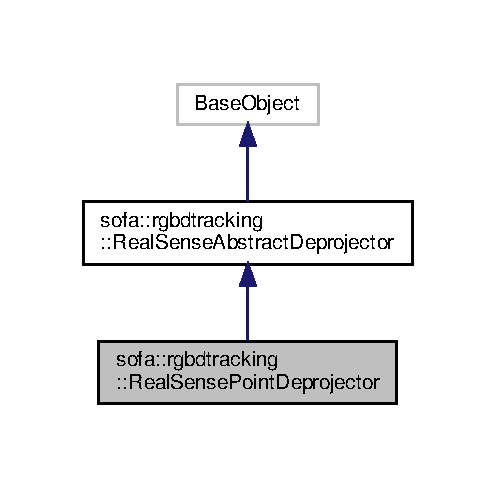
\includegraphics[width=238pt]{classsofa_1_1rgbdtracking_1_1_real_sense_point_deprojector__inherit__graph}
\end{center}
\end{figure}


Collaboration diagram for sofa\+:\+:rgbdtracking\+:\+:Real\+Sense\+Point\+Deprojector\+:\nopagebreak
\begin{figure}[H]
\begin{center}
\leavevmode
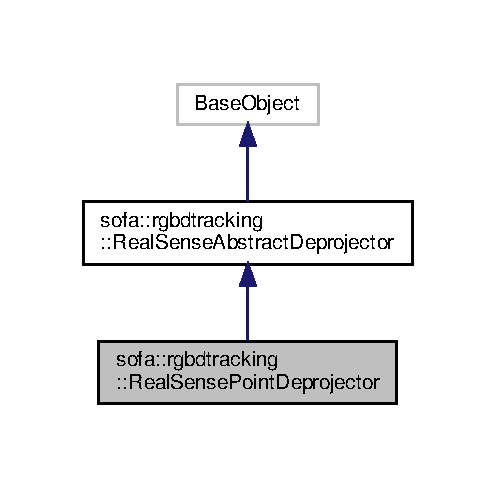
\includegraphics[width=238pt]{classsofa_1_1rgbdtracking_1_1_real_sense_point_deprojector__coll__graph}
\end{center}
\end{figure}
\subsection*{Public Types}
\begin{DoxyCompactItemize}
\item 
\mbox{\Hypertarget{classsofa_1_1rgbdtracking_1_1_real_sense_point_deprojector_a06e1fe2c0a7478ad85adf5d3add317f2}\label{classsofa_1_1rgbdtracking_1_1_real_sense_point_deprojector_a06e1fe2c0a7478ad85adf5d3add317f2}} 
typedef \hyperlink{classsofa_1_1rgbdtracking_1_1_real_sense_abstract_deprojector}{Real\+Sense\+Abstract\+Deprojector} {\bfseries Inherited}
\end{DoxyCompactItemize}
\subsection*{Public Member Functions}
\begin{DoxyCompactItemize}
\item 
\mbox{\Hypertarget{classsofa_1_1rgbdtracking_1_1_real_sense_point_deprojector_ac58e605830c9aec518aab80a94dbea3d}\label{classsofa_1_1rgbdtracking_1_1_real_sense_point_deprojector_ac58e605830c9aec518aab80a94dbea3d}} 
{\bfseries S\+O\+F\+A\+\_\+\+C\+L\+A\+SS} (\hyperlink{classsofa_1_1rgbdtracking_1_1_real_sense_point_deprojector}{Real\+Sense\+Point\+Deprojector}, Inherited)
\end{DoxyCompactItemize}
\subsection*{Public Attributes}
\begin{DoxyCompactItemize}
\item 
\mbox{\Hypertarget{classsofa_1_1rgbdtracking_1_1_real_sense_point_deprojector_a93e870b27e925201cd94f0e3c353ba94}\label{classsofa_1_1rgbdtracking_1_1_real_sense_point_deprojector_a93e870b27e925201cd94f0e3c353ba94}} 
Data$<$ helper\+::vector$<$ defaulttype\+::\+Vector2 $>$ $>$ \hyperlink{classsofa_1_1rgbdtracking_1_1_real_sense_point_deprojector_a93e870b27e925201cd94f0e3c353ba94}{d\+\_\+input}
\begin{DoxyCompactList}\small\item\em input list of 2d points to project in 3d \end{DoxyCompactList}\item 
\mbox{\Hypertarget{classsofa_1_1rgbdtracking_1_1_real_sense_point_deprojector_a66a99e38b3bdc576ed7da5df8307aa89}\label{classsofa_1_1rgbdtracking_1_1_real_sense_point_deprojector_a66a99e38b3bdc576ed7da5df8307aa89}} 
Data\+Callback {\bfseries c\+\_\+image}
\end{DoxyCompactItemize}


\subsection{Detailed Description}
The \hyperlink{classsofa_1_1rgbdtracking_1_1_real_sense_point_deprojector}{Real\+Sense\+Point\+Deprojector} class deprojects only a defined set of 2D points defined in d\+\_\+input (label input in sofa) from depth frame. 

The documentation for this class was generated from the following file\+:\begin{DoxyCompactItemize}
\item 
src/sofa/realsenseplugin/projector/Real\+Sense\+Point\+Deprojector.\+h\end{DoxyCompactItemize}

\hypertarget{classsofa_1_1rgbdtracking_1_1_real_sense_streamer}{}\section{sofa\+:\+:rgbdtracking\+:\+:Real\+Sense\+Streamer Class Reference}
\label{classsofa_1_1rgbdtracking_1_1_real_sense_streamer}\index{sofa\+::rgbdtracking\+::\+Real\+Sense\+Streamer@{sofa\+::rgbdtracking\+::\+Real\+Sense\+Streamer}}


The \hyperlink{classsofa_1_1rgbdtracking_1_1_real_sense_streamer}{Real\+Sense\+Streamer} class Abstract streamer used as a superclass for realsensecam and realsense virtual cam (used with multicam)  




{\ttfamily \#include $<$Real\+Sense\+Streamer.\+h$>$}



Inheritance diagram for sofa\+:\+:rgbdtracking\+:\+:Real\+Sense\+Streamer\+:
\nopagebreak
\begin{figure}[H]
\begin{center}
\leavevmode
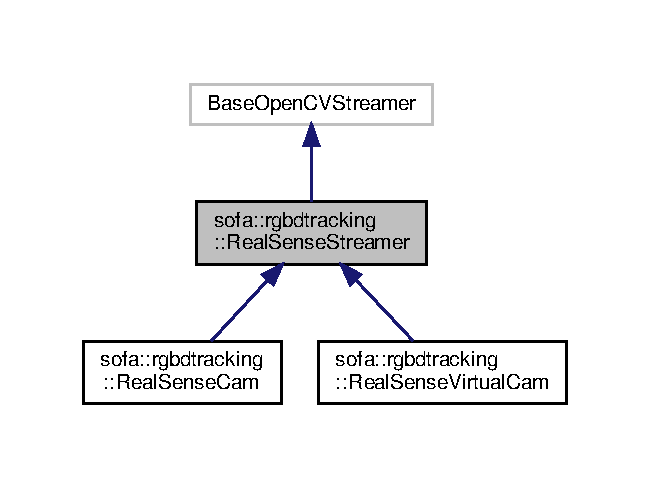
\includegraphics[width=312pt]{classsofa_1_1rgbdtracking_1_1_real_sense_streamer__inherit__graph}
\end{center}
\end{figure}


Collaboration diagram for sofa\+:\+:rgbdtracking\+:\+:Real\+Sense\+Streamer\+:
\nopagebreak
\begin{figure}[H]
\begin{center}
\leavevmode
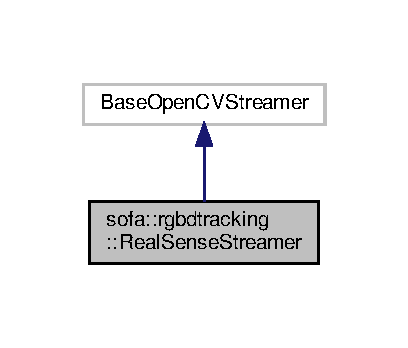
\includegraphics[width=196pt]{classsofa_1_1rgbdtracking_1_1_real_sense_streamer__coll__graph}
\end{center}
\end{figure}
\subsection*{Public Types}
\begin{DoxyCompactItemize}
\item 
\mbox{\Hypertarget{classsofa_1_1rgbdtracking_1_1_real_sense_streamer_a5f9ea54db5ca5e9cbbda378e0a93e07b}\label{classsofa_1_1rgbdtracking_1_1_real_sense_streamer_a5f9ea54db5ca5e9cbbda378e0a93e07b}} 
typedef opencvplugin\+::streamer\+::\+Base\+Open\+C\+V\+Streamer {\bfseries Inherited}
\end{DoxyCompactItemize}
\subsection*{Public Member Functions}
\begin{DoxyCompactItemize}
\item 
\mbox{\Hypertarget{classsofa_1_1rgbdtracking_1_1_real_sense_streamer_af9aacabd087d62ddcc436b9012d70e49}\label{classsofa_1_1rgbdtracking_1_1_real_sense_streamer_af9aacabd087d62ddcc436b9012d70e49}} 
{\bfseries S\+O\+F\+A\+\_\+\+C\+L\+A\+SS} (\hyperlink{classsofa_1_1rgbdtracking_1_1_real_sense_streamer}{Real\+Sense\+Streamer}, opencvplugin\+::streamer\+::\+Base\+Open\+C\+V\+Streamer)
\item 
void \hyperlink{classsofa_1_1rgbdtracking_1_1_real_sense_streamer_a3881452d7c26ef825640220be00fd034}{handle\+Event} (sofa\+::core\+::objectmodel\+::\+Event $\ast$event) override
\begin{DoxyCompactList}\small\item\em handle\+Event \+: Press i to push image to calibration image list, z to cancel, s to save \end{DoxyCompactList}\end{DoxyCompactItemize}
\subsection*{Public Attributes}
\begin{DoxyCompactItemize}
\item 
\mbox{\Hypertarget{classsofa_1_1rgbdtracking_1_1_real_sense_streamer_a4a21504b1c8de26cda98a7dd1b7d43d2}\label{classsofa_1_1rgbdtracking_1_1_real_sense_streamer_a4a21504b1c8de26cda98a7dd1b7d43d2}} 
Data$<$ opencvplugin\+::\+Image\+Data $>$ {\bfseries d\+\_\+color}
\item 
\mbox{\Hypertarget{classsofa_1_1rgbdtracking_1_1_real_sense_streamer_a9fbddc186f4026f029c509b49f5b16f5}\label{classsofa_1_1rgbdtracking_1_1_real_sense_streamer_a9fbddc186f4026f029c509b49f5b16f5}} 
Data$<$ opencvplugin\+::\+Image\+Data $>$ {\bfseries d\+\_\+depth}
\item 
\mbox{\Hypertarget{classsofa_1_1rgbdtracking_1_1_real_sense_streamer_a226a9797423c62c033f9f1961c00cb7c}\label{classsofa_1_1rgbdtracking_1_1_real_sense_streamer_a226a9797423c62c033f9f1961c00cb7c}} 
Data$<$ std\+::string $>$ {\bfseries d\+\_\+intrinsics}
\item 
\mbox{\Hypertarget{classsofa_1_1rgbdtracking_1_1_real_sense_streamer_a22b457cc55e1b6c1b0ce649c27c20ee6}\label{classsofa_1_1rgbdtracking_1_1_real_sense_streamer_a22b457cc55e1b6c1b0ce649c27c20ee6}} 
Data\+Callback {\bfseries c\+\_\+intrinsics}
\item 
\mbox{\Hypertarget{classsofa_1_1rgbdtracking_1_1_real_sense_streamer_a74e34153116c11df21f4b4630317e8b0}\label{classsofa_1_1rgbdtracking_1_1_real_sense_streamer_a74e34153116c11df21f4b4630317e8b0}} 
Data$<$ defaulttype\+::\+Vec4f $>$ {\bfseries d\+\_\+intrinsic\+Parameters}
\item 
\mbox{\Hypertarget{classsofa_1_1rgbdtracking_1_1_real_sense_streamer_a696eba343bf4d7d2f396b7506daab18f}\label{classsofa_1_1rgbdtracking_1_1_real_sense_streamer_a696eba343bf4d7d2f396b7506daab18f}} 
Data$<$ std\+::string $>$ {\bfseries d\+\_\+calibpath}
\item 
\mbox{\Hypertarget{classsofa_1_1rgbdtracking_1_1_real_sense_streamer_a01aa309d09c216db55a5596f10740803}\label{classsofa_1_1rgbdtracking_1_1_real_sense_streamer_a01aa309d09c216db55a5596f10740803}} 
std\+::vector$<$ cv\+::\+Mat $>$ {\bfseries calib\+\_\+imagelist}
\item 
\mbox{\Hypertarget{classsofa_1_1rgbdtracking_1_1_real_sense_streamer_a293f222ce3fe93aa62ae0475b714dd0d}\label{classsofa_1_1rgbdtracking_1_1_real_sense_streamer_a293f222ce3fe93aa62ae0475b714dd0d}} 
Data$<$ int $>$ {\bfseries depth\+Scale}
\item 
\mbox{\Hypertarget{classsofa_1_1rgbdtracking_1_1_real_sense_streamer_ac8353a52ed5997b5180bcc99f384c351}\label{classsofa_1_1rgbdtracking_1_1_real_sense_streamer_ac8353a52ed5997b5180bcc99f384c351}} 
rs2\+::video\+\_\+frame $\ast$ {\bfseries color}
\item 
\mbox{\Hypertarget{classsofa_1_1rgbdtracking_1_1_real_sense_streamer_ae5a0ca709953b170ffb596abedd51eed}\label{classsofa_1_1rgbdtracking_1_1_real_sense_streamer_ae5a0ca709953b170ffb596abedd51eed}} 
rs2\+::depth\+\_\+frame $\ast$ {\bfseries depth}
\item 
\mbox{\Hypertarget{classsofa_1_1rgbdtracking_1_1_real_sense_streamer_a9f25b9a13cfab87d3e9878da5f2b6e32}\label{classsofa_1_1rgbdtracking_1_1_real_sense_streamer_a9f25b9a13cfab87d3e9878da5f2b6e32}} 
rs2\+\_\+intrinsics {\bfseries cam\+\_\+intrinsics}
\end{DoxyCompactItemize}
\subsection*{Protected Member Functions}
\begin{DoxyCompactItemize}
\item 
\mbox{\Hypertarget{classsofa_1_1rgbdtracking_1_1_real_sense_streamer_a1db9130e1444a18c5a5a3f19e8dc32da}\label{classsofa_1_1rgbdtracking_1_1_real_sense_streamer_a1db9130e1444a18c5a5a3f19e8dc32da}} 
void \hyperlink{classsofa_1_1rgbdtracking_1_1_real_sense_streamer_a1db9130e1444a18c5a5a3f19e8dc32da}{write\+Intrinsics\+To\+File} ()
\begin{DoxyCompactList}\small\item\em write\+Intrinsics\+To\+File \+: intrinsics path file in sofa data needs to be set \end{DoxyCompactList}\item 
\mbox{\Hypertarget{classsofa_1_1rgbdtracking_1_1_real_sense_streamer_ae7f7303c5cc323868d3bcc36d13c8689}\label{classsofa_1_1rgbdtracking_1_1_real_sense_streamer_ae7f7303c5cc323868d3bcc36d13c8689}} 
void {\bfseries write\+Intrinsics} (std\+::string filename, const rs2\+\_\+intrinsics \&cam\+\_\+intrinsics)
\item 
rs2\+::frameset \hyperlink{classsofa_1_1rgbdtracking_1_1_real_sense_streamer_a3ea622968695865d727d67b72e8363c7}{wait\+\_\+for\+\_\+frame} (rs2\+::pipeline \&pipe)
\begin{DoxyCompactList}\small\item\em wait\+\_\+for\+\_\+frame \+: waits for rgbd frame from realsense \end{DoxyCompactList}\item 
\mbox{\Hypertarget{classsofa_1_1rgbdtracking_1_1_real_sense_streamer_aac7fbd7301db4731d78aaf89a2022a01}\label{classsofa_1_1rgbdtracking_1_1_real_sense_streamer_aac7fbd7301db4731d78aaf89a2022a01}} 
void \hyperlink{classsofa_1_1rgbdtracking_1_1_real_sense_streamer_aac7fbd7301db4731d78aaf89a2022a01}{frame\+\_\+to\+\_\+cvmat} (rs2\+::video\+\_\+frame color, rs2\+::depth\+\_\+frame depth, cv\+::\+Mat \&bgr\+\_\+image, cv\+::\+Mat \&depth8)
\begin{DoxyCompactList}\small\item\em convert R\+GB \& D rs2\+::frames to cv\+::\+Mat and stores them in data container \end{DoxyCompactList}\end{DoxyCompactItemize}


\subsection{Detailed Description}
The \hyperlink{classsofa_1_1rgbdtracking_1_1_real_sense_streamer}{Real\+Sense\+Streamer} class Abstract streamer used as a superclass for realsensecam and realsense virtual cam (used with multicam) 

\subsection{Member Function Documentation}
\mbox{\Hypertarget{classsofa_1_1rgbdtracking_1_1_real_sense_streamer_a3881452d7c26ef825640220be00fd034}\label{classsofa_1_1rgbdtracking_1_1_real_sense_streamer_a3881452d7c26ef825640220be00fd034}} 
\index{sofa\+::rgbdtracking\+::\+Real\+Sense\+Streamer@{sofa\+::rgbdtracking\+::\+Real\+Sense\+Streamer}!handle\+Event@{handle\+Event}}
\index{handle\+Event@{handle\+Event}!sofa\+::rgbdtracking\+::\+Real\+Sense\+Streamer@{sofa\+::rgbdtracking\+::\+Real\+Sense\+Streamer}}
\subsubsection{\texorpdfstring{handle\+Event()}{handleEvent()}}
{\footnotesize\ttfamily void sofa\+::rgbdtracking\+::\+Real\+Sense\+Streamer\+::handle\+Event (\begin{DoxyParamCaption}\item[{sofa\+::core\+::objectmodel\+::\+Event $\ast$}]{event }\end{DoxyParamCaption})\hspace{0.3cm}{\ttfamily [inline]}, {\ttfamily [override]}}



handle\+Event \+: Press i to push image to calibration image list, z to cancel, s to save 


\begin{DoxyParams}{Parameters}
{\em event} & \\
\hline
\end{DoxyParams}
\mbox{\Hypertarget{classsofa_1_1rgbdtracking_1_1_real_sense_streamer_a3ea622968695865d727d67b72e8363c7}\label{classsofa_1_1rgbdtracking_1_1_real_sense_streamer_a3ea622968695865d727d67b72e8363c7}} 
\index{sofa\+::rgbdtracking\+::\+Real\+Sense\+Streamer@{sofa\+::rgbdtracking\+::\+Real\+Sense\+Streamer}!wait\+\_\+for\+\_\+frame@{wait\+\_\+for\+\_\+frame}}
\index{wait\+\_\+for\+\_\+frame@{wait\+\_\+for\+\_\+frame}!sofa\+::rgbdtracking\+::\+Real\+Sense\+Streamer@{sofa\+::rgbdtracking\+::\+Real\+Sense\+Streamer}}
\subsubsection{\texorpdfstring{wait\+\_\+for\+\_\+frame()}{wait\_for\_frame()}}
{\footnotesize\ttfamily rs2\+::frameset sofa\+::rgbdtracking\+::\+Real\+Sense\+Streamer\+::wait\+\_\+for\+\_\+frame (\begin{DoxyParamCaption}\item[{rs2\+::pipeline \&}]{pipe }\end{DoxyParamCaption})\hspace{0.3cm}{\ttfamily [inline]}, {\ttfamily [protected]}}



wait\+\_\+for\+\_\+frame \+: waits for rgbd frame from realsense 


\begin{DoxyParams}{Parameters}
{\em pipe} & \\
\hline
\end{DoxyParams}
\begin{DoxyReturn}{Returns}
realsense current frameset 
\end{DoxyReturn}


The documentation for this class was generated from the following file\+:\begin{DoxyCompactItemize}
\item 
src/sofa/realsenseplugin/streamer/Real\+Sense\+Streamer.\+h\end{DoxyCompactItemize}

\hypertarget{classsofa_1_1rgbdtracking_1_1_real_sense_virtual_cam}{}\section{sofa\+:\+:rgbdtracking\+:\+:Real\+Sense\+Virtual\+Cam Class Reference}
\label{classsofa_1_1rgbdtracking_1_1_real_sense_virtual_cam}\index{sofa\+::rgbdtracking\+::\+Real\+Sense\+Virtual\+Cam@{sofa\+::rgbdtracking\+::\+Real\+Sense\+Virtual\+Cam}}


The \hyperlink{classsofa_1_1rgbdtracking_1_1_real_sense_virtual_cam}{Real\+Sense\+Virtual\+Cam} class virtual cam instanciated from multicam component.  




{\ttfamily \#include $<$Real\+Sense\+Multi\+Cam.\+h$>$}



Inheritance diagram for sofa\+:\+:rgbdtracking\+:\+:Real\+Sense\+Virtual\+Cam\+:
\nopagebreak
\begin{figure}[H]
\begin{center}
\leavevmode
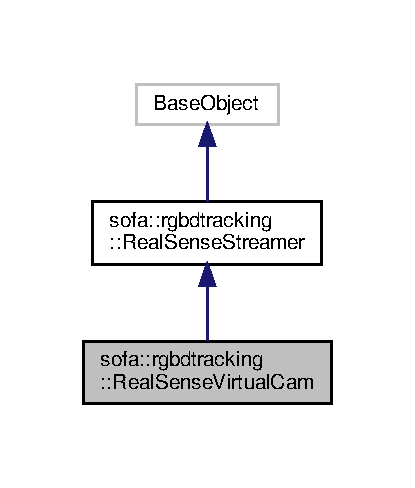
\includegraphics[width=199pt]{classsofa_1_1rgbdtracking_1_1_real_sense_virtual_cam__inherit__graph}
\end{center}
\end{figure}


Collaboration diagram for sofa\+:\+:rgbdtracking\+:\+:Real\+Sense\+Virtual\+Cam\+:
\nopagebreak
\begin{figure}[H]
\begin{center}
\leavevmode
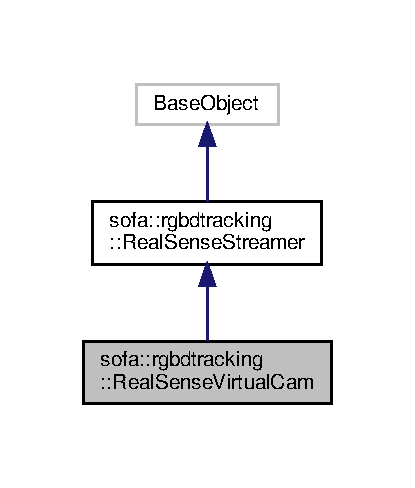
\includegraphics[width=199pt]{classsofa_1_1rgbdtracking_1_1_real_sense_virtual_cam__coll__graph}
\end{center}
\end{figure}
\subsection*{Public Types}
\begin{DoxyCompactItemize}
\item 
\mbox{\Hypertarget{classsofa_1_1rgbdtracking_1_1_real_sense_virtual_cam_aaf38bfd843842903f4b1e4457af3240f}\label{classsofa_1_1rgbdtracking_1_1_real_sense_virtual_cam_aaf38bfd843842903f4b1e4457af3240f}} 
typedef \hyperlink{classsofa_1_1rgbdtracking_1_1_real_sense_streamer}{Real\+Sense\+Streamer} {\bfseries Inherited}
\end{DoxyCompactItemize}
\subsection*{Public Member Functions}
\begin{DoxyCompactItemize}
\item 
\mbox{\Hypertarget{classsofa_1_1rgbdtracking_1_1_real_sense_virtual_cam_ac20d0286ccdd5caff30412db342814dc}\label{classsofa_1_1rgbdtracking_1_1_real_sense_virtual_cam_ac20d0286ccdd5caff30412db342814dc}} 
{\bfseries S\+O\+F\+A\+\_\+\+C\+L\+A\+SS} (\hyperlink{classsofa_1_1rgbdtracking_1_1_real_sense_virtual_cam}{Real\+Sense\+Virtual\+Cam}, \hyperlink{classsofa_1_1rgbdtracking_1_1_real_sense_streamer}{Inherited})
\item 
\mbox{\Hypertarget{classsofa_1_1rgbdtracking_1_1_real_sense_virtual_cam_a673da2cd1e90f9448b458066e2f81eee}\label{classsofa_1_1rgbdtracking_1_1_real_sense_virtual_cam_a673da2cd1e90f9448b458066e2f81eee}} 
{\bfseries Real\+Sense\+Virtual\+Cam} (std\+::string serialnum)
\item 
\mbox{\Hypertarget{classsofa_1_1rgbdtracking_1_1_real_sense_virtual_cam_adc341623bbde6d3cc70f2cdc8a0263ef}\label{classsofa_1_1rgbdtracking_1_1_real_sense_virtual_cam_adc341623bbde6d3cc70f2cdc8a0263ef}} 
void {\bfseries init} ()
\item 
\mbox{\Hypertarget{classsofa_1_1rgbdtracking_1_1_real_sense_virtual_cam_ac4eceae3e70c1cdb0f597b45e439cdc1}\label{classsofa_1_1rgbdtracking_1_1_real_sense_virtual_cam_ac4eceae3e70c1cdb0f597b45e439cdc1}} 
void {\bfseries decode\+Image} (cv\+::\+Mat \&img)
\end{DoxyCompactItemize}
\subsection*{Public Attributes}
\begin{DoxyCompactItemize}
\item 
\mbox{\Hypertarget{classsofa_1_1rgbdtracking_1_1_real_sense_virtual_cam_aebfd00b71c1ce8a5505a602386dd3864}\label{classsofa_1_1rgbdtracking_1_1_real_sense_virtual_cam_aebfd00b71c1ce8a5505a602386dd3864}} 
rs2\+::pipeline {\bfseries pipe}
\item 
\mbox{\Hypertarget{classsofa_1_1rgbdtracking_1_1_real_sense_virtual_cam_a45ccc29bedb1dd6f5357a0a3ecb8f8bb}\label{classsofa_1_1rgbdtracking_1_1_real_sense_virtual_cam_a45ccc29bedb1dd6f5357a0a3ecb8f8bb}} 
std\+::string {\bfseries serial}
\end{DoxyCompactItemize}
\subsection*{Additional Inherited Members}


\subsection{Detailed Description}
The \hyperlink{classsofa_1_1rgbdtracking_1_1_real_sense_virtual_cam}{Real\+Sense\+Virtual\+Cam} class virtual cam instanciated from multicam component. 

The documentation for this class was generated from the following file\+:\begin{DoxyCompactItemize}
\item 
src/sofa/realsenseplugin/streamer/Real\+Sense\+Multi\+Cam.\+h\end{DoxyCompactItemize}

\chapter{File Documentation}
\hypertarget{cv-helpers_8hpp}{}\section{src/sofa/realsenseplugin/cv-\/helpers.hpp File Reference}
\label{cv-helpers_8hpp}\index{src/sofa/realsenseplugin/cv-\/helpers.\+hpp@{src/sofa/realsenseplugin/cv-\/helpers.\+hpp}}
{\ttfamily \#include $<$librealsense2/rs.\+hpp$>$}\newline
{\ttfamily \#include $<$opencv2/opencv.\+hpp$>$}\newline
Include dependency graph for cv-\/helpers.hpp\+:\nopagebreak
\begin{figure}[H]
\begin{center}
\leavevmode
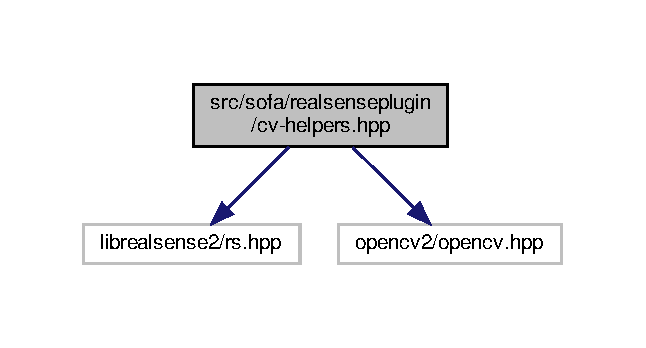
\includegraphics[width=310pt]{cv-helpers_8hpp__incl}
\end{center}
\end{figure}
This graph shows which files directly or indirectly include this file\+:\nopagebreak
\begin{figure}[H]
\begin{center}
\leavevmode
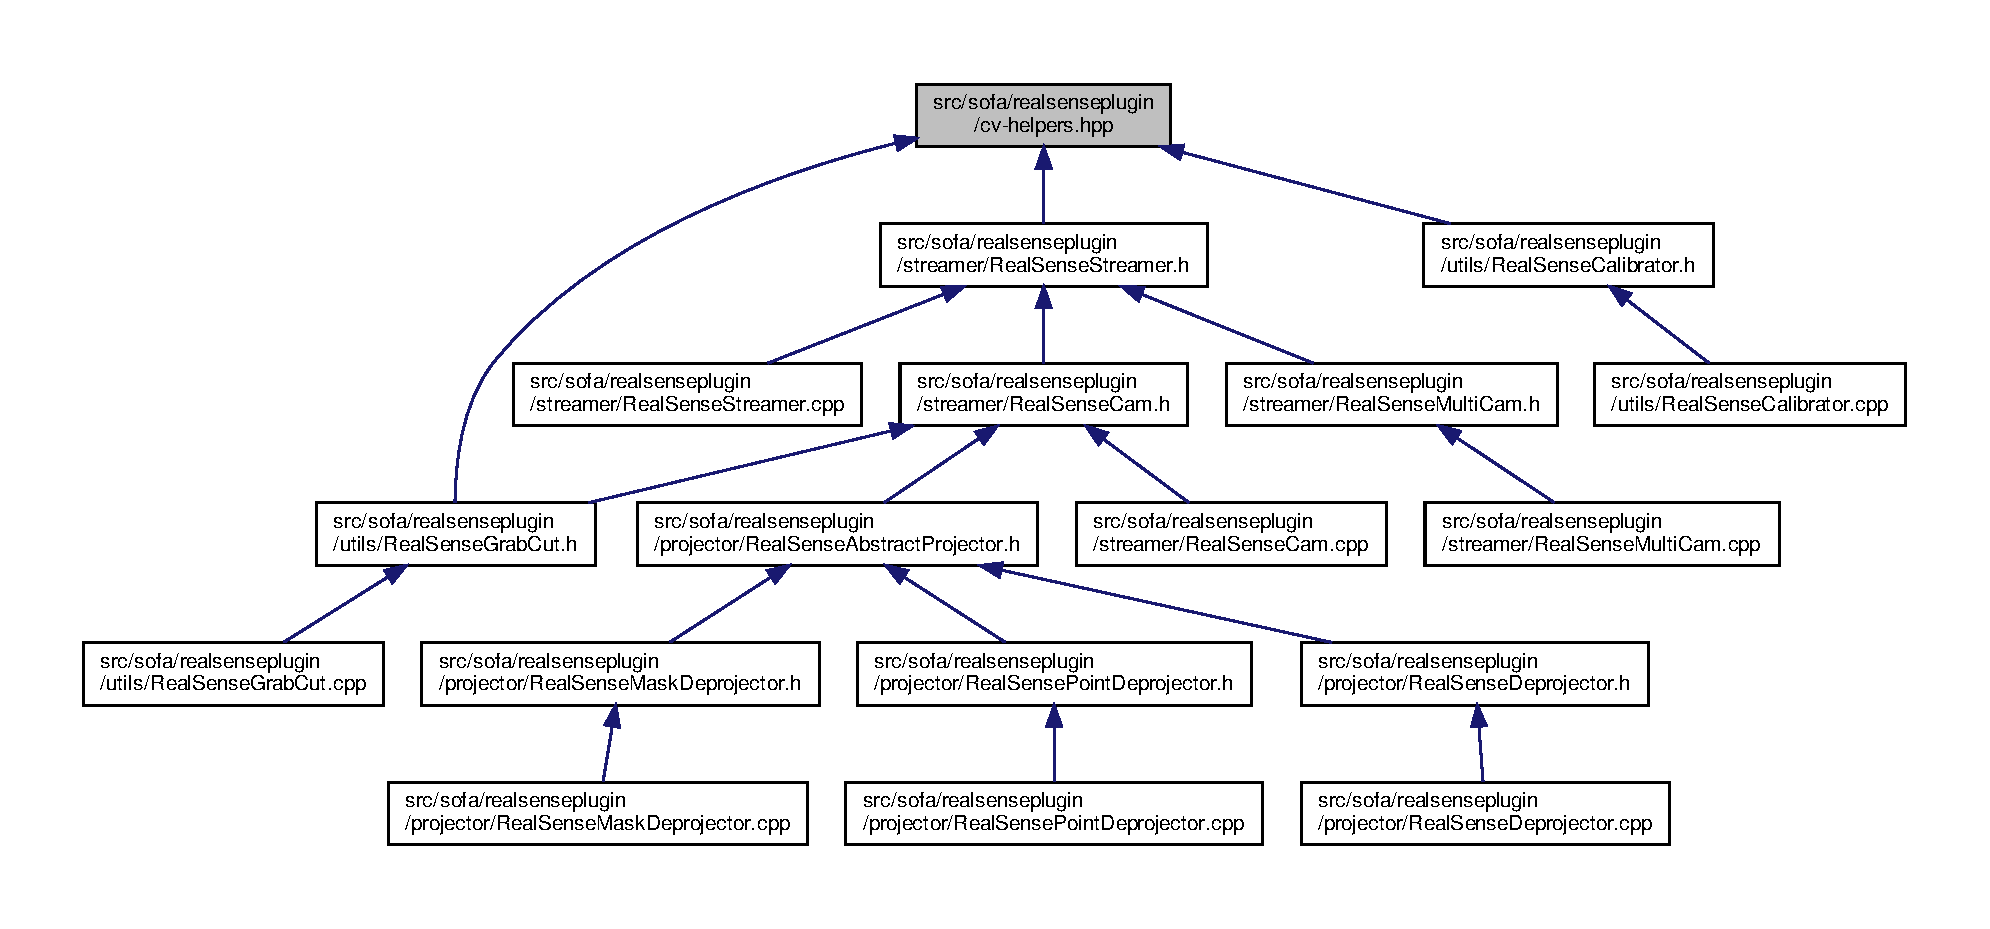
\includegraphics[width=350pt]{cv-helpers_8hpp__dep__incl}
\end{center}
\end{figure}
\subsection*{Functions}
\begin{DoxyCompactItemize}
\item 
cv\+::\+Mat \hyperlink{cv-helpers_8hpp_a9f7789d2d48f2a70a8075f81e6b79a85}{frame\+\_\+to\+\_\+mat} (const rs2\+::frame \&f)
\item 
cv\+::\+Mat \hyperlink{cv-helpers_8hpp_a7e9d970007238e5460324343841905aa}{depth\+\_\+frame\+\_\+to\+\_\+meters} (const rs2\+::pipeline \&pipe, const rs2\+::depth\+\_\+frame \&f)
\end{DoxyCompactItemize}


\subsection{Function Documentation}
\mbox{\Hypertarget{cv-helpers_8hpp_a7e9d970007238e5460324343841905aa}\label{cv-helpers_8hpp_a7e9d970007238e5460324343841905aa}} 
\index{cv-\/helpers.\+hpp@{cv-\/helpers.\+hpp}!depth\+\_\+frame\+\_\+to\+\_\+meters@{depth\+\_\+frame\+\_\+to\+\_\+meters}}
\index{depth\+\_\+frame\+\_\+to\+\_\+meters@{depth\+\_\+frame\+\_\+to\+\_\+meters}!cv-\/helpers.\+hpp@{cv-\/helpers.\+hpp}}
\subsubsection{\texorpdfstring{depth\+\_\+frame\+\_\+to\+\_\+meters()}{depth\_frame\_to\_meters()}}
{\footnotesize\ttfamily cv\+::\+Mat depth\+\_\+frame\+\_\+to\+\_\+meters (\begin{DoxyParamCaption}\item[{const rs2\+::pipeline \&}]{pipe,  }\item[{const rs2\+::depth\+\_\+frame \&}]{f }\end{DoxyParamCaption})\hspace{0.3cm}{\ttfamily [inline]}}

\mbox{\Hypertarget{cv-helpers_8hpp_a9f7789d2d48f2a70a8075f81e6b79a85}\label{cv-helpers_8hpp_a9f7789d2d48f2a70a8075f81e6b79a85}} 
\index{cv-\/helpers.\+hpp@{cv-\/helpers.\+hpp}!frame\+\_\+to\+\_\+mat@{frame\+\_\+to\+\_\+mat}}
\index{frame\+\_\+to\+\_\+mat@{frame\+\_\+to\+\_\+mat}!cv-\/helpers.\+hpp@{cv-\/helpers.\+hpp}}
\subsubsection{\texorpdfstring{frame\+\_\+to\+\_\+mat()}{frame\_to\_mat()}}
{\footnotesize\ttfamily cv\+::\+Mat frame\+\_\+to\+\_\+mat (\begin{DoxyParamCaption}\item[{const rs2\+::frame \&}]{f }\end{DoxyParamCaption})\hspace{0.3cm}{\ttfamily [inline]}}


\hypertarget{init_plugin_8cpp}{}\section{src/sofa/realsenseplugin/init\+Plugin.cpp File Reference}
\label{init_plugin_8cpp}\index{src/sofa/realsenseplugin/init\+Plugin.\+cpp@{src/sofa/realsenseplugin/init\+Plugin.\+cpp}}
{\ttfamily \#include $<$string$>$}\newline
{\ttfamily \#include $<$stdio.\+h$>$}\newline
{\ttfamily \#include $<$sofa/helper/system/\+File\+Repository.\+h$>$}\newline
{\ttfamily \#include $<$sofa/helper/system/\+Set\+Directory.\+h$>$}\newline
{\ttfamily \#include $<$sofa/core/\+Object\+Factory.\+h$>$}\newline
Include dependency graph for init\+Plugin.\+cpp\+:\nopagebreak
\begin{figure}[H]
\begin{center}
\leavevmode
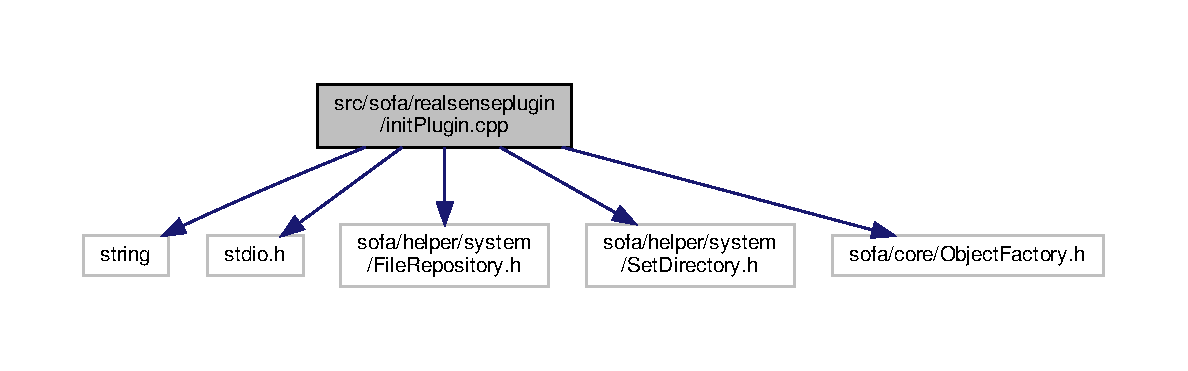
\includegraphics[width=350pt]{init_plugin_8cpp__incl}
\end{center}
\end{figure}
\subsection*{Namespaces}
\begin{DoxyCompactItemize}
\item 
 \hyperlink{namespacesofa}{sofa}
\item 
 \hyperlink{namespacesofa_1_1rgbdtracking}{sofa\+::rgbdtracking}
\end{DoxyCompactItemize}
\subsection*{Macros}
\begin{DoxyCompactItemize}
\item 
\#define \hyperlink{init_plugin_8cpp_a2a280bfe12bc6e732a7c4d3d62443a14}{Q}(x)~\#x
\item 
\#define \hyperlink{init_plugin_8cpp_a2117b58e19182dff91ad3558e650541d}{Q\+U\+O\+TE}(x)~\hyperlink{init_plugin_8cpp_a2a280bfe12bc6e732a7c4d3d62443a14}{Q}(x)
\item 
\#define \hyperlink{init_plugin_8cpp_a91ba46c856cef51c949da946f5e7d134}{P\+L\+U\+G\+I\+N\+\_\+\+D\+A\+T\+A\+\_\+\+D\+I\+R\+\_\+}~\char`\"{}\char`\"{}
\end{DoxyCompactItemize}
\subsection*{Functions}
\begin{DoxyCompactItemize}
\item 
void \hyperlink{namespacesofa_1_1rgbdtracking_a596d0c2a2b98cc3dd0091e933070ecce}{sofa\+::rgbdtracking\+::init\+External\+Module} ()
\item 
const char $\ast$ \hyperlink{namespacesofa_1_1rgbdtracking_a71f655bffd81cca5c72c2fc4a0aa72d3}{sofa\+::rgbdtracking\+::get\+Module\+Name} ()
\item 
const char $\ast$ \hyperlink{namespacesofa_1_1rgbdtracking_ac45b27a5c97c1ec95aa078ac013bcca7}{sofa\+::rgbdtracking\+::get\+Module\+Version} ()
\item 
const char $\ast$ \hyperlink{namespacesofa_1_1rgbdtracking_a3d5dee9f71234c539f75d68e90eb4120}{sofa\+::rgbdtracking\+::get\+Module\+License} ()
\item 
const char $\ast$ \hyperlink{namespacesofa_1_1rgbdtracking_a720f3a55d983babc84a6f4ce8ce7d67f}{sofa\+::rgbdtracking\+::get\+Module\+Description} ()
\item 
const char $\ast$ \hyperlink{namespacesofa_1_1rgbdtracking_a7687b3685880c0911d3f8f2e97000f5d}{sofa\+::rgbdtracking\+::get\+Module\+Component\+List} ()
\end{DoxyCompactItemize}


\subsection{Macro Definition Documentation}
\mbox{\Hypertarget{init_plugin_8cpp_a91ba46c856cef51c949da946f5e7d134}\label{init_plugin_8cpp_a91ba46c856cef51c949da946f5e7d134}} 
\index{init\+Plugin.\+cpp@{init\+Plugin.\+cpp}!P\+L\+U\+G\+I\+N\+\_\+\+D\+A\+T\+A\+\_\+\+D\+I\+R\+\_\+@{P\+L\+U\+G\+I\+N\+\_\+\+D\+A\+T\+A\+\_\+\+D\+I\+R\+\_\+}}
\index{P\+L\+U\+G\+I\+N\+\_\+\+D\+A\+T\+A\+\_\+\+D\+I\+R\+\_\+@{P\+L\+U\+G\+I\+N\+\_\+\+D\+A\+T\+A\+\_\+\+D\+I\+R\+\_\+}!init\+Plugin.\+cpp@{init\+Plugin.\+cpp}}
\subsubsection{\texorpdfstring{P\+L\+U\+G\+I\+N\+\_\+\+D\+A\+T\+A\+\_\+\+D\+I\+R\+\_\+}{PLUGIN\_DATA\_DIR\_}}
{\footnotesize\ttfamily \#define P\+L\+U\+G\+I\+N\+\_\+\+D\+A\+T\+A\+\_\+\+D\+I\+R\+\_\+~\char`\"{}\char`\"{}}

\mbox{\Hypertarget{init_plugin_8cpp_a2a280bfe12bc6e732a7c4d3d62443a14}\label{init_plugin_8cpp_a2a280bfe12bc6e732a7c4d3d62443a14}} 
\index{init\+Plugin.\+cpp@{init\+Plugin.\+cpp}!Q@{Q}}
\index{Q@{Q}!init\+Plugin.\+cpp@{init\+Plugin.\+cpp}}
\subsubsection{\texorpdfstring{Q}{Q}}
{\footnotesize\ttfamily \#define Q(\begin{DoxyParamCaption}\item[{}]{x }\end{DoxyParamCaption})~\#x}

\mbox{\Hypertarget{init_plugin_8cpp_a2117b58e19182dff91ad3558e650541d}\label{init_plugin_8cpp_a2117b58e19182dff91ad3558e650541d}} 
\index{init\+Plugin.\+cpp@{init\+Plugin.\+cpp}!Q\+U\+O\+TE@{Q\+U\+O\+TE}}
\index{Q\+U\+O\+TE@{Q\+U\+O\+TE}!init\+Plugin.\+cpp@{init\+Plugin.\+cpp}}
\subsubsection{\texorpdfstring{Q\+U\+O\+TE}{QUOTE}}
{\footnotesize\ttfamily \#define Q\+U\+O\+TE(\begin{DoxyParamCaption}\item[{}]{x }\end{DoxyParamCaption})~\hyperlink{init_plugin_8cpp_a2a280bfe12bc6e732a7c4d3d62443a14}{Q}(x)}


\hypertarget{_real_sense_abstract_projector_8h}{}\section{src/sofa/realsenseplugin/projector/\+Real\+Sense\+Abstract\+Projector.h File Reference}
\label{_real_sense_abstract_projector_8h}\index{src/sofa/realsenseplugin/projector/\+Real\+Sense\+Abstract\+Projector.\+h@{src/sofa/realsenseplugin/projector/\+Real\+Sense\+Abstract\+Projector.\+h}}
{\ttfamily \#include $<$sofa/defaulttype/\+Vec.\+h$>$}\newline
{\ttfamily \#include $<$sofa/core/objectmodel/\+Base\+Object.\+h$>$}\newline
{\ttfamily \#include $<$sofa/core/objectmodel/\+Data\+File\+Name.\+h$>$}\newline
{\ttfamily \#include $<$sofa/core/objectmodel/\+Mouse\+Event.\+h$>$}\newline
{\ttfamily \#include $<$sofa/core/visual/\+Visual\+Params.\+h$>$}\newline
{\ttfamily \#include $<$sofa/defaulttype/\+Bounding\+Box.\+h$>$}\newline
{\ttfamily \#include $<$sofa/core/objectmodel/\+Event.\+h$>$}\newline
{\ttfamily \#include $<$sofa/simulation/\+Animate\+Begin\+Event.\+h$>$}\newline
{\ttfamily \#include $<$sofa/simulation/\+Animate\+End\+Event.\+h$>$}\newline
{\ttfamily \#include $<$sofa/defaulttype/\+Mat.\+h$>$}\newline
{\ttfamily \#include $<$sofa/defaulttype/\+Quat.\+h$>$}\newline
{\ttfamily \#include $<$sofa/helper/rmath.\+h$>$}\newline
{\ttfamily \#include $<$sofa/helper/\+Options\+Group.\+h$>$}\newline
{\ttfamily \#include $<$librealsense2/rs.\+hpp$>$}\newline
{\ttfamily \#include $<$librealsense2/rsutil.\+h$>$}\newline
{\ttfamily \#include $<$opencv2/opencv.\+hpp$>$}\newline
{\ttfamily \#include $<$opencv2/imgproc.\+hpp$>$}\newline
{\ttfamily \#include $<$fstream$>$}\newline
{\ttfamily \#include $<$algorithm$>$}\newline
{\ttfamily \#include $<$iostream$>$}\newline
{\ttfamily \#include $<$string$>$}\newline
{\ttfamily \#include $<$map$>$}\newline
{\ttfamily \#include $<$sofa/opencvplugin/\+Open\+C\+V\+Widget.\+h$>$}\newline
{\ttfamily \#include $<$sofa/\+P\+C\+L\+Plugin/\+Point\+Cloud\+Data.\+h$>$}\newline
{\ttfamily \#include $<$sofa/realsenseplugin/streamer/\+Real\+Sense\+Cam.\+h$>$}\newline
{\ttfamily \#include $<$sofa/realsenseplugin/projector/\+Real\+Sense\+Dist\+Frame.\+h$>$}\newline
Include dependency graph for Real\+Sense\+Abstract\+Projector.\+h\+:\nopagebreak
\begin{figure}[H]
\begin{center}
\leavevmode
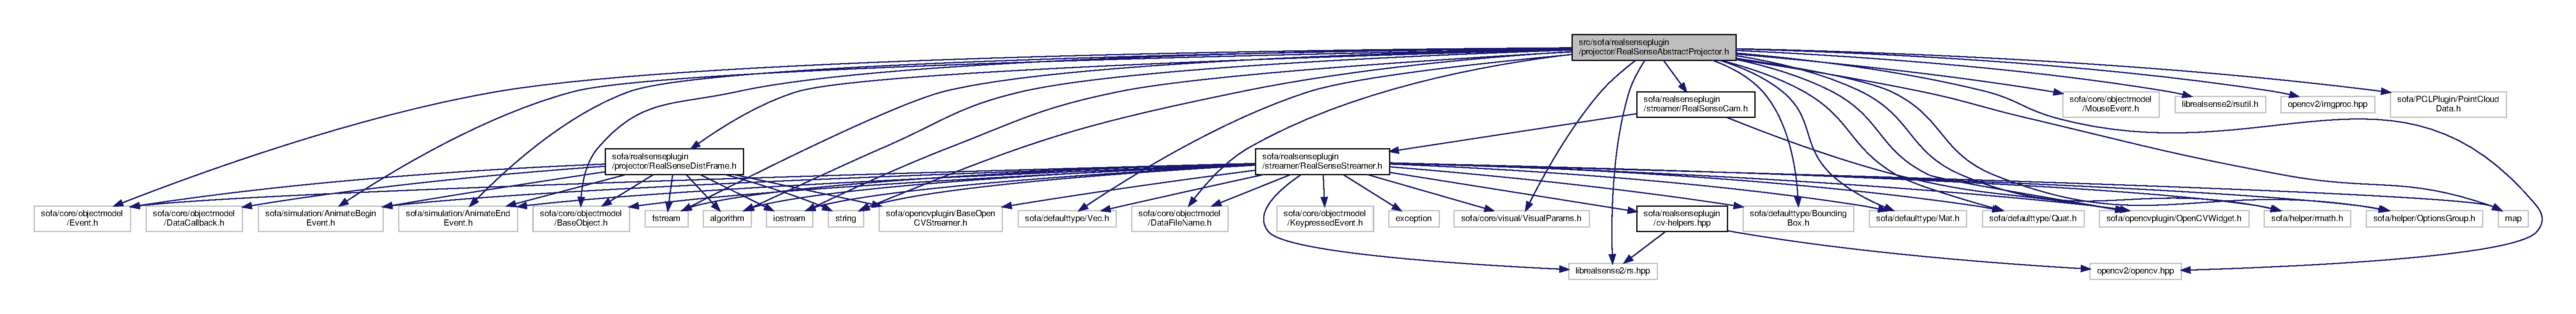
\includegraphics[width=350pt]{_real_sense_abstract_projector_8h__incl}
\end{center}
\end{figure}
This graph shows which files directly or indirectly include this file\+:\nopagebreak
\begin{figure}[H]
\begin{center}
\leavevmode
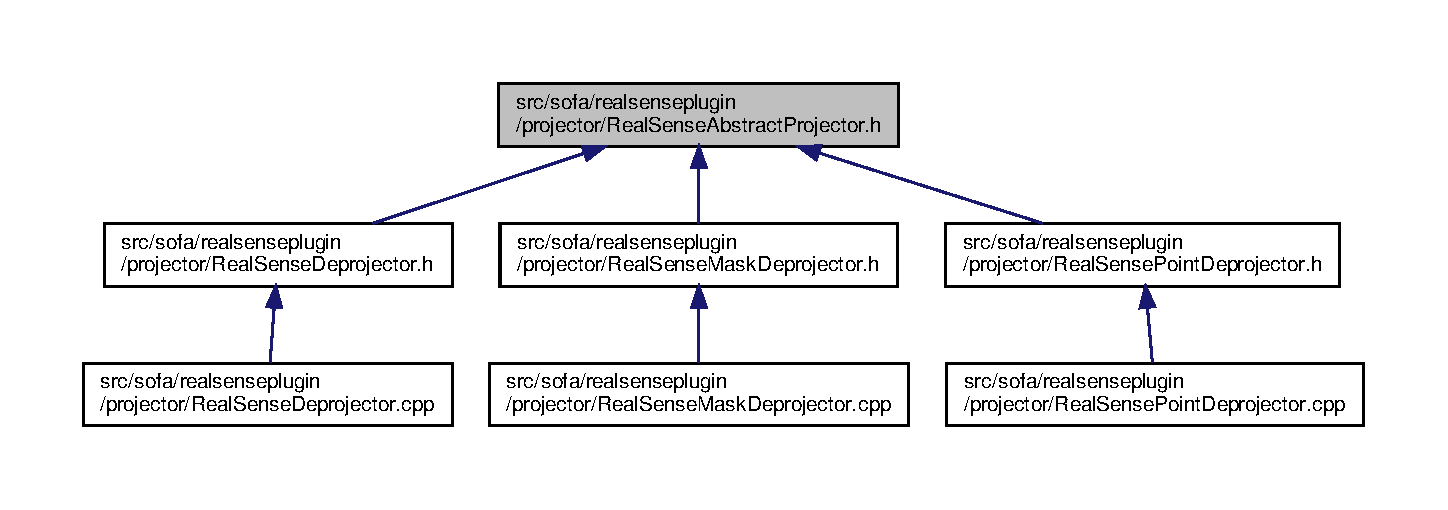
\includegraphics[width=350pt]{_real_sense_abstract_projector_8h__dep__incl}
\end{center}
\end{figure}
\subsection*{Classes}
\begin{DoxyCompactItemize}
\item 
class \hyperlink{classsofa_1_1rgbdtracking_1_1_real_sense_abstract_deprojector}{sofa\+::rgbdtracking\+::\+Real\+Sense\+Abstract\+Deprojector}
\end{DoxyCompactItemize}
\subsection*{Namespaces}
\begin{DoxyCompactItemize}
\item 
 \hyperlink{namespacesofa}{sofa}
\item 
 \hyperlink{namespacesofa_1_1rgbdtracking}{sofa\+::rgbdtracking}
\end{DoxyCompactItemize}

\hypertarget{_real_sense_deprojector_8cpp}{}\section{src/sofa/realsenseplugin/projector/\+Real\+Sense\+Deprojector.cpp File Reference}
\label{_real_sense_deprojector_8cpp}\index{src/sofa/realsenseplugin/projector/\+Real\+Sense\+Deprojector.\+cpp@{src/sofa/realsenseplugin/projector/\+Real\+Sense\+Deprojector.\+cpp}}
{\ttfamily \#include \char`\"{}Real\+Sense\+Deprojector.\+h\char`\"{}}\newline
{\ttfamily \#include $<$sofa/core/\+Object\+Factory.\+h$>$}\newline
Include dependency graph for Real\+Sense\+Deprojector.\+cpp\+:\nopagebreak
\begin{figure}[H]
\begin{center}
\leavevmode
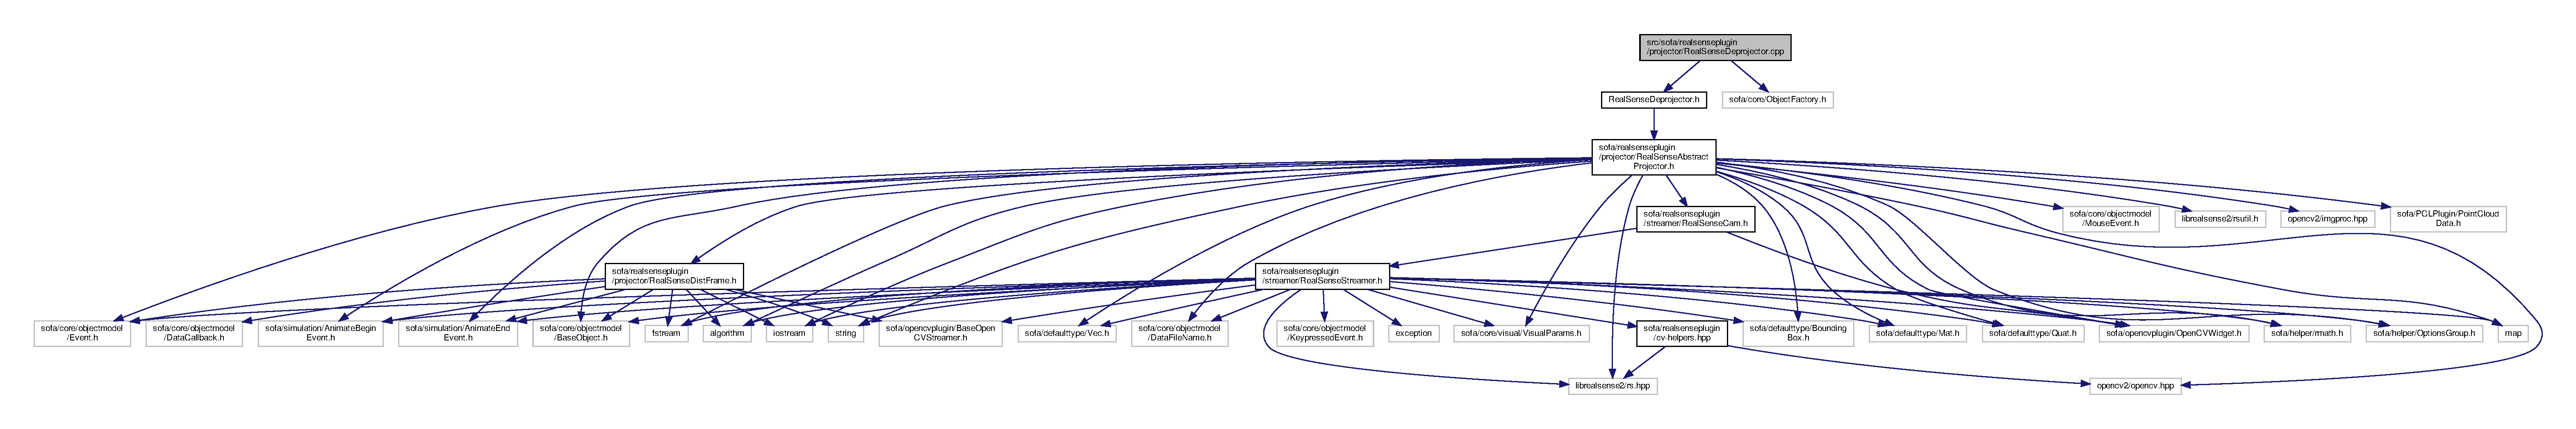
\includegraphics[width=350pt]{_real_sense_deprojector_8cpp__incl}
\end{center}
\end{figure}
\subsection*{Namespaces}
\begin{DoxyCompactItemize}
\item 
 \hyperlink{namespacesofa}{sofa}
\item 
 \hyperlink{namespacesofa_1_1rgbdtracking}{sofa\+::rgbdtracking}
\end{DoxyCompactItemize}
\subsection*{Variables}
\begin{DoxyCompactItemize}
\item 
int \hyperlink{namespacesofa_1_1rgbdtracking_ac3f6d225dbe5a6782bfbb716bc3940e9}{sofa\+::rgbdtracking\+::\+R\+S\+Deprojector\+Class}
\end{DoxyCompactItemize}

\hypertarget{_real_sense_deprojector_8h}{}\section{src/sofa/realsenseplugin/projector/\+Real\+Sense\+Deprojector.h File Reference}
\label{_real_sense_deprojector_8h}\index{src/sofa/realsenseplugin/projector/\+Real\+Sense\+Deprojector.\+h@{src/sofa/realsenseplugin/projector/\+Real\+Sense\+Deprojector.\+h}}
{\ttfamily \#include $<$sofa/realsenseplugin/projector/\+Real\+Sense\+Abstract\+Projector.\+h$>$}\newline
Include dependency graph for Real\+Sense\+Deprojector.\+h\+:\nopagebreak
\begin{figure}[H]
\begin{center}
\leavevmode
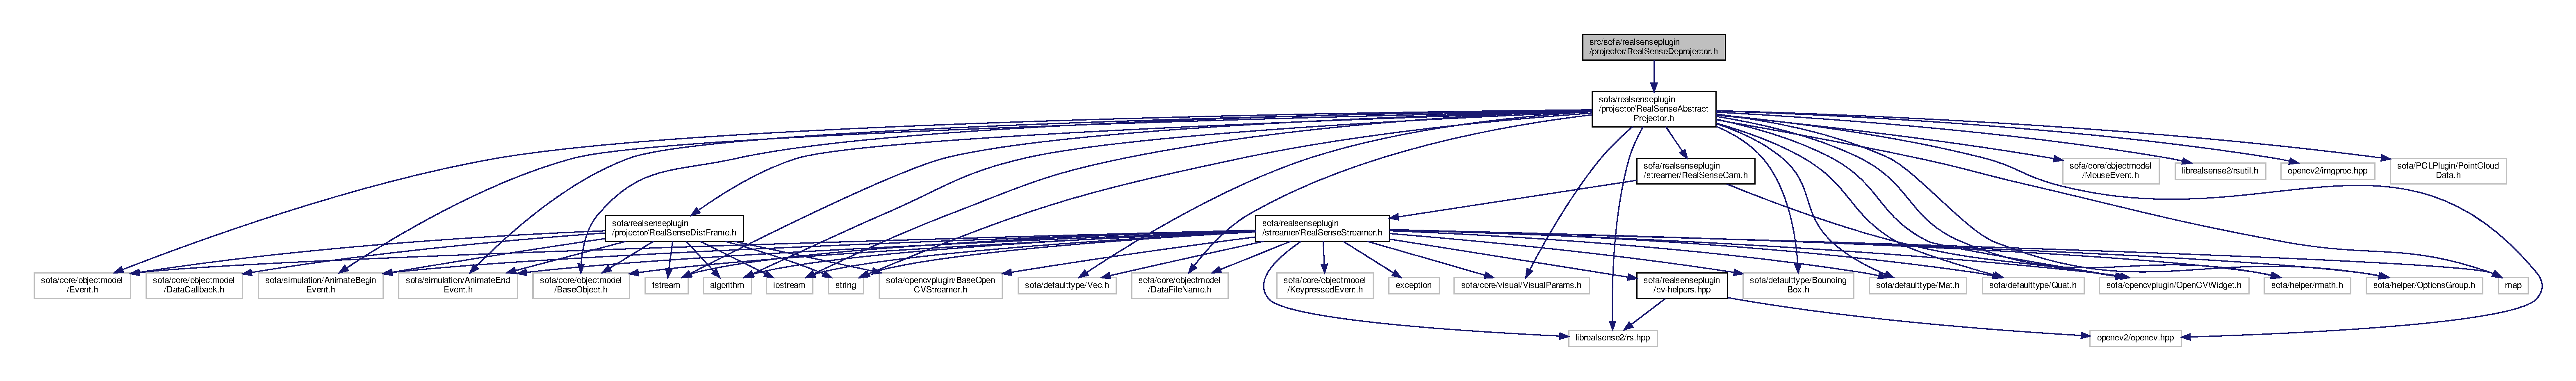
\includegraphics[width=350pt]{_real_sense_deprojector_8h__incl}
\end{center}
\end{figure}
This graph shows which files directly or indirectly include this file\+:\nopagebreak
\begin{figure}[H]
\begin{center}
\leavevmode
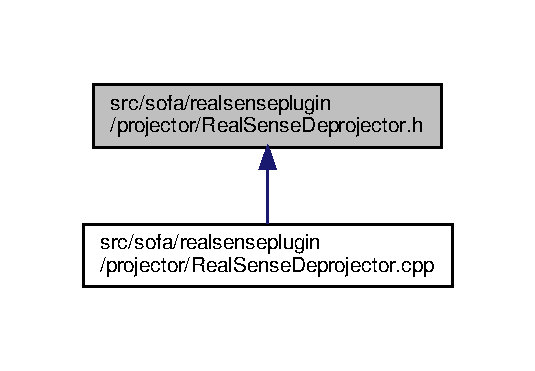
\includegraphics[width=257pt]{_real_sense_deprojector_8h__dep__incl}
\end{center}
\end{figure}
\subsection*{Classes}
\begin{DoxyCompactItemize}
\item 
class \hyperlink{classsofa_1_1rgbdtracking_1_1_real_sense_deprojector}{sofa\+::rgbdtracking\+::\+Real\+Sense\+Deprojector}
\begin{DoxyCompactList}\small\item\em The \hyperlink{classsofa_1_1rgbdtracking_1_1_real_sense_deprojector}{Real\+Sense\+Deprojector} class Online / Offline 2\+D-\/3D deprojection of whole rgb-\/d scene. \end{DoxyCompactList}\end{DoxyCompactItemize}
\subsection*{Namespaces}
\begin{DoxyCompactItemize}
\item 
 \hyperlink{namespacesofa}{sofa}
\item 
 \hyperlink{namespacesofa_1_1rgbdtracking}{sofa\+::rgbdtracking}
\end{DoxyCompactItemize}

\hypertarget{_real_sense_dist_frame_8cpp}{}\section{src/sofa/realsenseplugin/projector/\+Real\+Sense\+Dist\+Frame.cpp File Reference}
\label{_real_sense_dist_frame_8cpp}\index{src/sofa/realsenseplugin/projector/\+Real\+Sense\+Dist\+Frame.\+cpp@{src/sofa/realsenseplugin/projector/\+Real\+Sense\+Dist\+Frame.\+cpp}}
{\ttfamily \#include \char`\"{}Real\+Sense\+Dist\+Frame.\+h\char`\"{}}\newline
{\ttfamily \#include $<$sofa/core/\+Object\+Factory.\+h$>$}\newline
Include dependency graph for Real\+Sense\+Dist\+Frame.\+cpp\+:\nopagebreak
\begin{figure}[H]
\begin{center}
\leavevmode
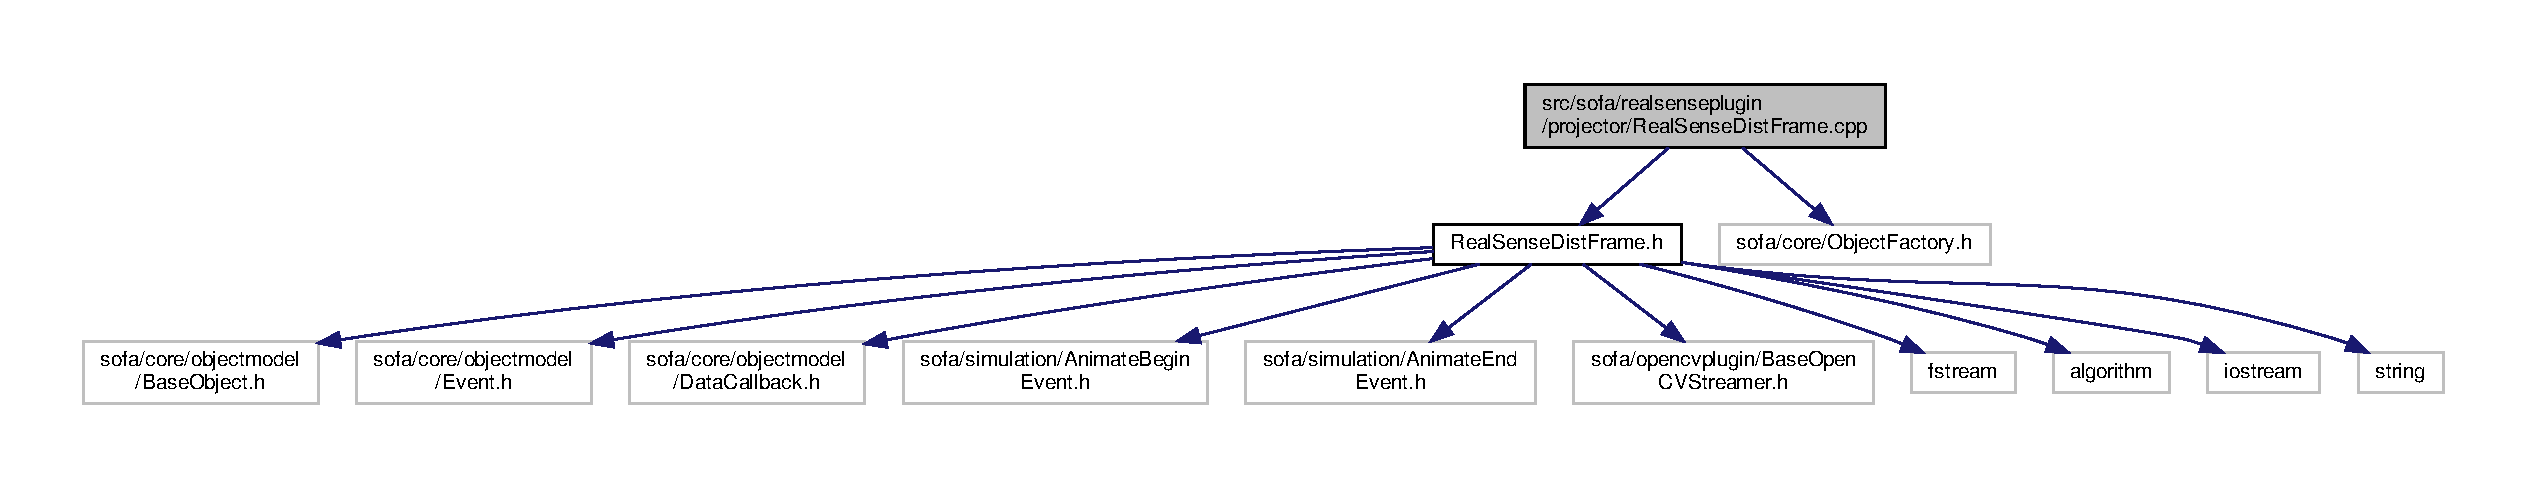
\includegraphics[width=350pt]{_real_sense_dist_frame_8cpp__incl}
\end{center}
\end{figure}
\subsection*{Namespaces}
\begin{DoxyCompactItemize}
\item 
 \hyperlink{namespacesofa}{sofa}
\item 
 \hyperlink{namespacesofa_1_1rgbdtracking}{sofa\+::rgbdtracking}
\end{DoxyCompactItemize}
\subsection*{Variables}
\begin{DoxyCompactItemize}
\item 
int \hyperlink{namespacesofa_1_1rgbdtracking_a1b9f5fecf5affbe66747355df84f3eba}{sofa\+::rgbdtracking\+::\+Dist\+Frame\+Exporter\+Class}
\item 
int \hyperlink{namespacesofa_1_1rgbdtracking_a7d552ae238bb3e3f0323220bd43f38d5}{sofa\+::rgbdtracking\+::\+Dist\+Frame\+Streamer\+Class}
\end{DoxyCompactItemize}

\hypertarget{_real_sense_dist_frame_8h}{}\section{src/sofa/realsenseplugin/projector/\+Real\+Sense\+Dist\+Frame.h File Reference}
\label{_real_sense_dist_frame_8h}\index{src/sofa/realsenseplugin/projector/\+Real\+Sense\+Dist\+Frame.\+h@{src/sofa/realsenseplugin/projector/\+Real\+Sense\+Dist\+Frame.\+h}}
{\ttfamily \#include $<$sofa/core/objectmodel/\+Base\+Object.\+h$>$}\newline
{\ttfamily \#include $<$sofa/core/objectmodel/\+Event.\+h$>$}\newline
{\ttfamily \#include $<$sofa/core/objectmodel/\+Data\+Callback.\+h$>$}\newline
{\ttfamily \#include $<$sofa/simulation/\+Animate\+Begin\+Event.\+h$>$}\newline
{\ttfamily \#include $<$sofa/simulation/\+Animate\+End\+Event.\+h$>$}\newline
{\ttfamily \#include $<$sofa/opencvplugin/\+Base\+Open\+C\+V\+Streamer.\+h$>$}\newline
{\ttfamily \#include $<$fstream$>$}\newline
{\ttfamily \#include $<$algorithm$>$}\newline
{\ttfamily \#include $<$iostream$>$}\newline
{\ttfamily \#include $<$string$>$}\newline
Include dependency graph for Real\+Sense\+Dist\+Frame.\+h\+:\nopagebreak
\begin{figure}[H]
\begin{center}
\leavevmode
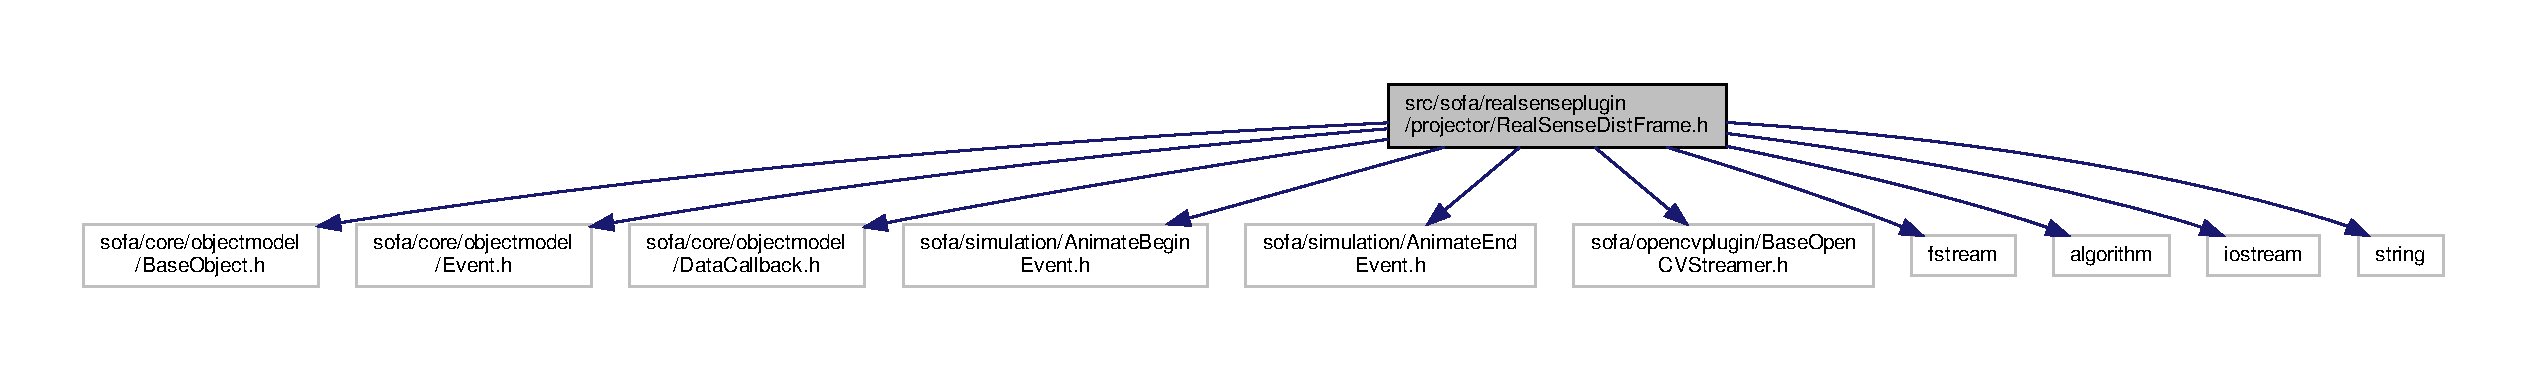
\includegraphics[width=350pt]{_real_sense_dist_frame_8h__incl}
\end{center}
\end{figure}
This graph shows which files directly or indirectly include this file\+:\nopagebreak
\begin{figure}[H]
\begin{center}
\leavevmode
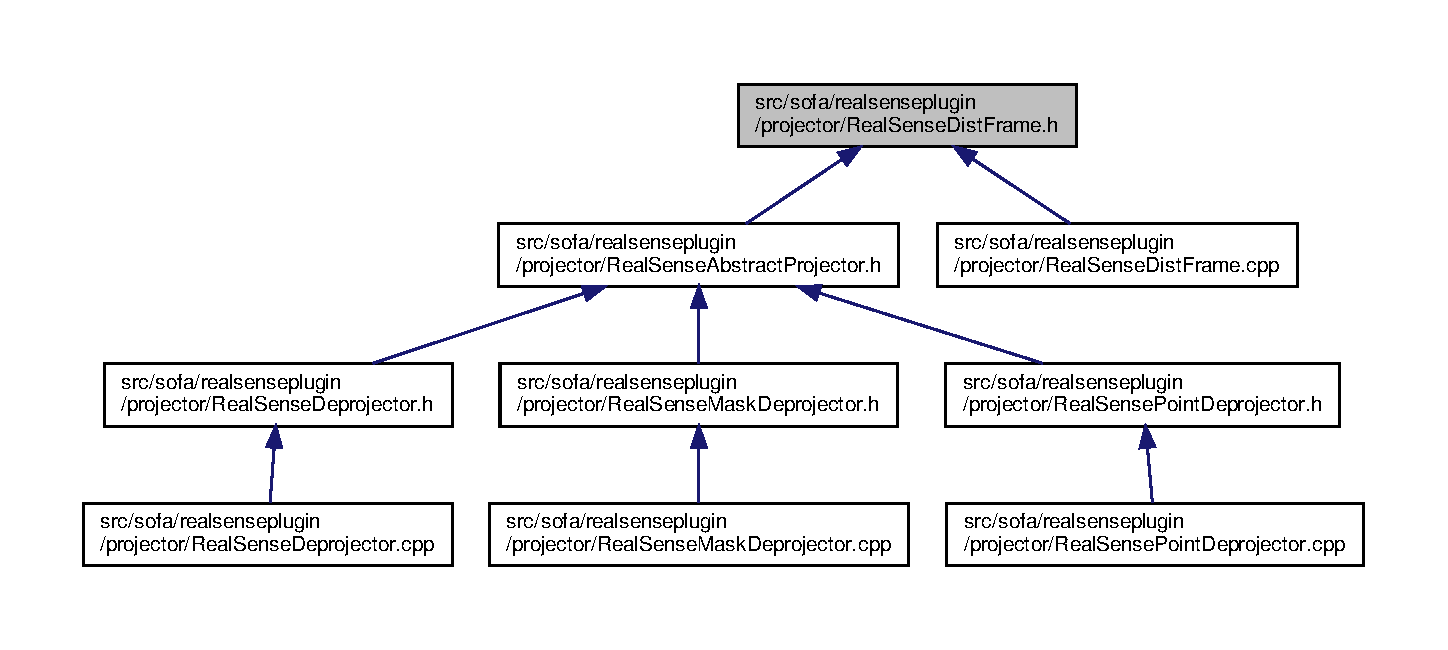
\includegraphics[width=350pt]{_real_sense_dist_frame_8h__dep__incl}
\end{center}
\end{figure}
\subsection*{Classes}
\begin{DoxyCompactItemize}
\item 
class \hyperlink{classsofa_1_1rgbdtracking_1_1_real_sense_dist_frame}{sofa\+::rgbdtracking\+::\+Real\+Sense\+Dist\+Frame}
\begin{DoxyCompactList}\small\item\em The \hyperlink{classsofa_1_1rgbdtracking_1_1_real_sense_dist_frame}{Real\+Sense\+Dist\+Frame} class Used for distance frame usage as sofa data by components. \end{DoxyCompactList}\item 
struct \hyperlink{structsofa_1_1rgbdtracking_1_1_real_sense_dist_frame_1_1_real_sense_dist_struct}{sofa\+::rgbdtracking\+::\+Real\+Sense\+Dist\+Frame\+::\+Real\+Sense\+Dist\+Struct}
\item 
class \hyperlink{classsofa_1_1rgbdtracking_1_1_real_sense_dist_frame_exporter}{sofa\+::rgbdtracking\+::\+Real\+Sense\+Dist\+Frame\+Exporter}
\begin{DoxyCompactList}\small\item\em The \hyperlink{classsofa_1_1rgbdtracking_1_1_real_sense_dist_frame_exporter}{Real\+Sense\+Dist\+Frame\+Exporter} class exports distance frames to file for offline processing. \end{DoxyCompactList}\item 
class \hyperlink{classsofa_1_1rgbdtracking_1_1_real_sense_dist_frame_streamer}{sofa\+::rgbdtracking\+::\+Real\+Sense\+Dist\+Frame\+Streamer}
\begin{DoxyCompactList}\small\item\em The \hyperlink{classsofa_1_1rgbdtracking_1_1_real_sense_dist_frame_streamer}{Real\+Sense\+Dist\+Frame\+Streamer} class Streams through distance frames in a file Implements Base\+Open\+C\+V\+Streamer. \end{DoxyCompactList}\end{DoxyCompactItemize}
\subsection*{Namespaces}
\begin{DoxyCompactItemize}
\item 
 \hyperlink{namespacesofa}{sofa}
\item 
 \hyperlink{namespacesofa_1_1rgbdtracking}{sofa\+::rgbdtracking}
\end{DoxyCompactItemize}
\subsection*{Typedefs}
\begin{DoxyCompactItemize}
\item 
using \hyperlink{namespacesofa_1_1rgbdtracking_a00834a9204a667746fef9a402ccbfb55}{sofa\+::rgbdtracking\+::\+Data\+Callback} = core\+::objectmodel\+::\+Data\+Callback
\end{DoxyCompactItemize}

\hypertarget{_real_sense_mask_deprojector_8cpp}{}\section{src/sofa/realsenseplugin/projector/\+Real\+Sense\+Mask\+Deprojector.cpp File Reference}
\label{_real_sense_mask_deprojector_8cpp}\index{src/sofa/realsenseplugin/projector/\+Real\+Sense\+Mask\+Deprojector.\+cpp@{src/sofa/realsenseplugin/projector/\+Real\+Sense\+Mask\+Deprojector.\+cpp}}
{\ttfamily \#include \char`\"{}Real\+Sense\+Mask\+Deprojector.\+h\char`\"{}}\newline
{\ttfamily \#include $<$sofa/core/\+Object\+Factory.\+h$>$}\newline
Include dependency graph for Real\+Sense\+Mask\+Deprojector.\+cpp\+:\nopagebreak
\begin{figure}[H]
\begin{center}
\leavevmode
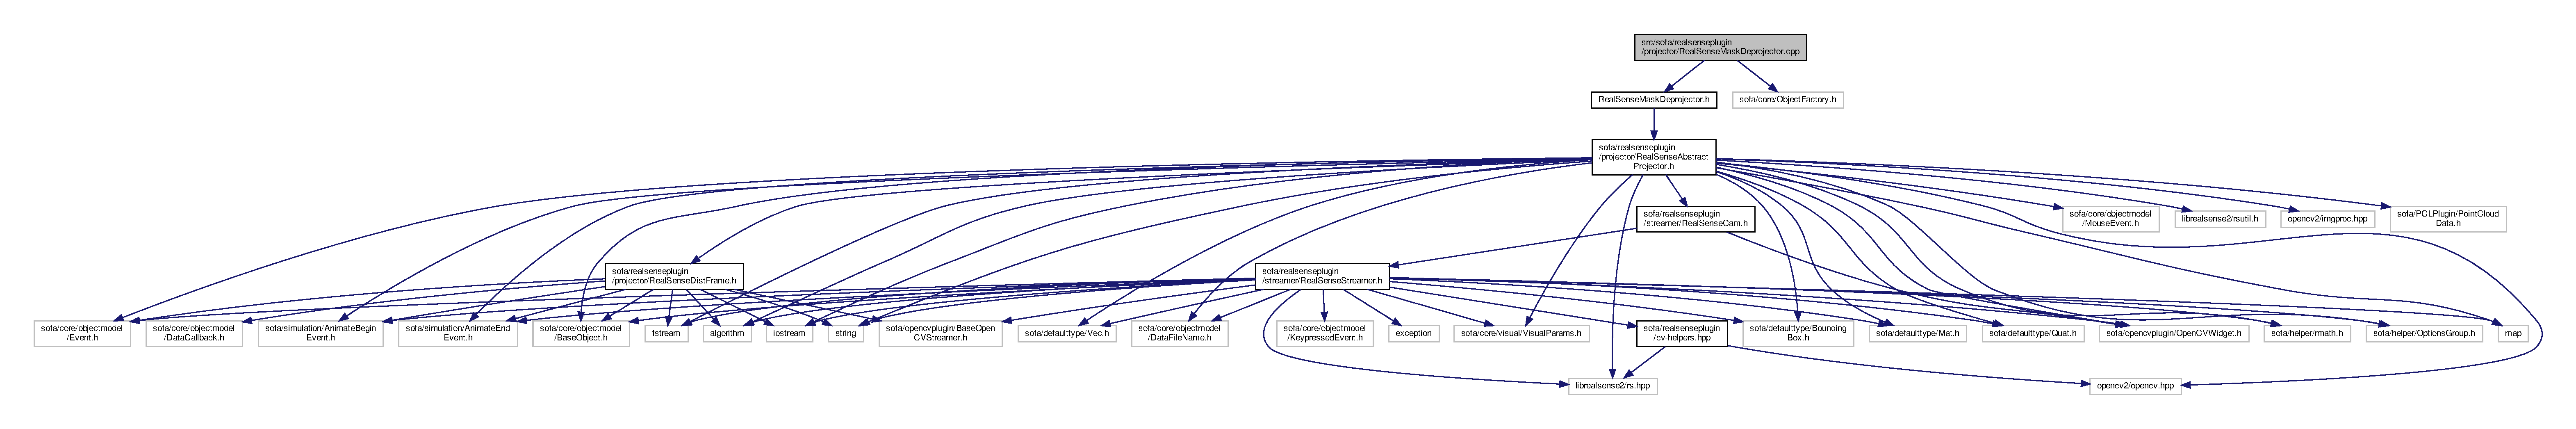
\includegraphics[width=350pt]{_real_sense_mask_deprojector_8cpp__incl}
\end{center}
\end{figure}
\subsection*{Namespaces}
\begin{DoxyCompactItemize}
\item 
 \hyperlink{namespacesofa}{sofa}
\item 
 \hyperlink{namespacesofa_1_1rgbdtracking}{sofa\+::rgbdtracking}
\end{DoxyCompactItemize}
\subsection*{Variables}
\begin{DoxyCompactItemize}
\item 
int \hyperlink{namespacesofa_1_1rgbdtracking_a585e4b070b41993d28e4c727bcd0b836}{sofa\+::rgbdtracking\+::\+R\+S\+Mask\+Deprojector\+Class}
\end{DoxyCompactItemize}

\hypertarget{_real_sense_mask_deprojector_8h}{}\section{src/sofa/realsenseplugin/projector/\+Real\+Sense\+Mask\+Deprojector.h File Reference}
\label{_real_sense_mask_deprojector_8h}\index{src/sofa/realsenseplugin/projector/\+Real\+Sense\+Mask\+Deprojector.\+h@{src/sofa/realsenseplugin/projector/\+Real\+Sense\+Mask\+Deprojector.\+h}}
{\ttfamily \#include $<$sofa/realsenseplugin/projector/\+Real\+Sense\+Abstract\+Projector.\+h$>$}\newline
Include dependency graph for Real\+Sense\+Mask\+Deprojector.\+h\+:\nopagebreak
\begin{figure}[H]
\begin{center}
\leavevmode
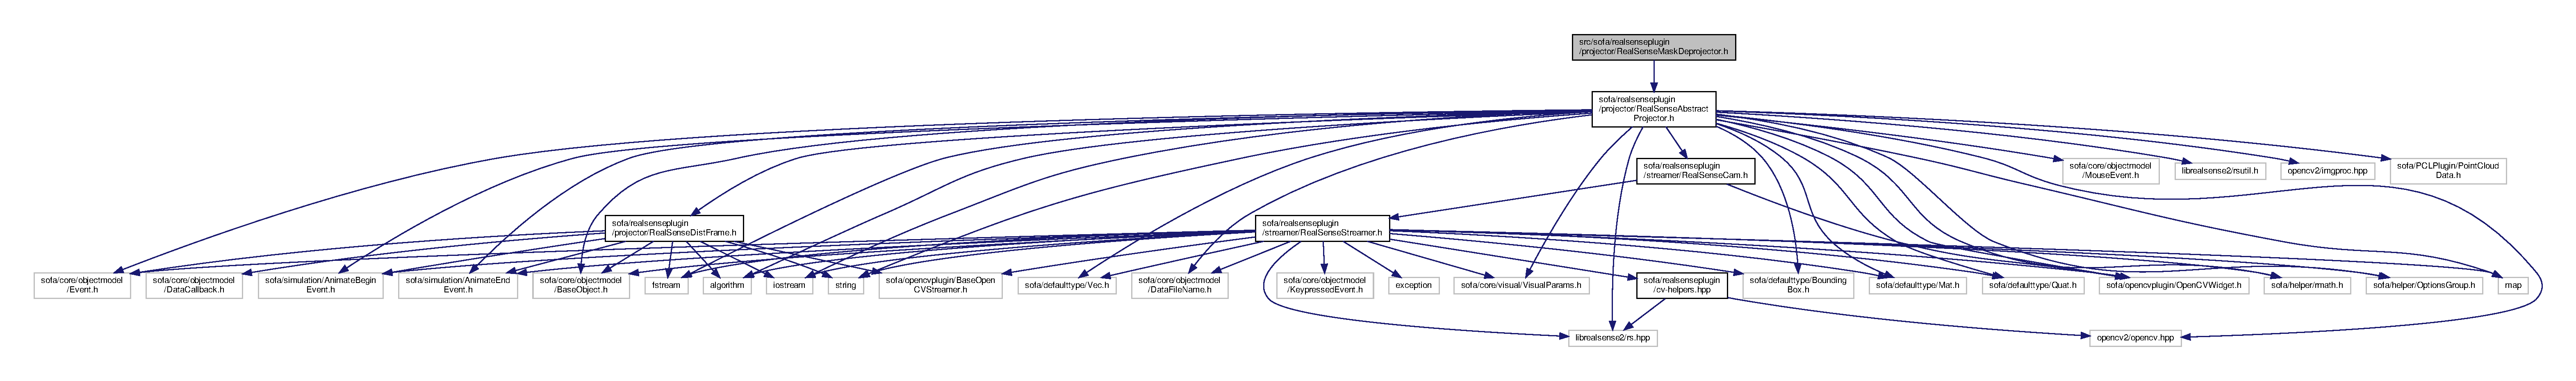
\includegraphics[width=350pt]{_real_sense_mask_deprojector_8h__incl}
\end{center}
\end{figure}
This graph shows which files directly or indirectly include this file\+:\nopagebreak
\begin{figure}[H]
\begin{center}
\leavevmode
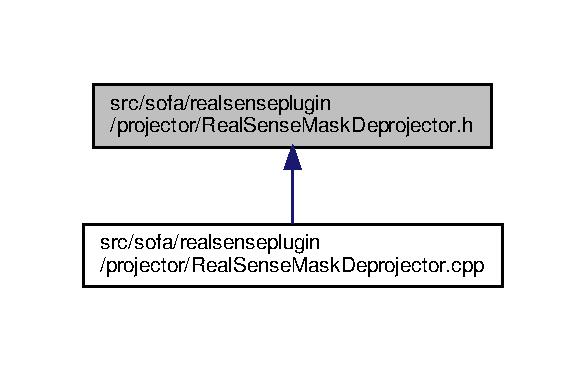
\includegraphics[width=281pt]{_real_sense_mask_deprojector_8h__dep__incl}
\end{center}
\end{figure}
\subsection*{Classes}
\begin{DoxyCompactItemize}
\item 
class \hyperlink{classsofa_1_1rgbdtracking_1_1_real_sense_mask_deprojector}{sofa\+::rgbdtracking\+::\+Real\+Sense\+Mask\+Deprojector}
\begin{DoxyCompactList}\small\item\em The \hyperlink{classsofa_1_1rgbdtracking_1_1_real_sense_mask_deprojector}{Real\+Sense\+Mask\+Deprojector} class deprojects a set of points depending on a 2D binary mask defined as an image in d\+\_\+input (label input in sofa) \end{DoxyCompactList}\end{DoxyCompactItemize}
\subsection*{Namespaces}
\begin{DoxyCompactItemize}
\item 
 \hyperlink{namespacesofa}{sofa}
\item 
 \hyperlink{namespacesofa_1_1rgbdtracking}{sofa\+::rgbdtracking}
\end{DoxyCompactItemize}

\hypertarget{_real_sense_point_deprojector_8cpp}{}\section{src/sofa/realsenseplugin/projector/\+Real\+Sense\+Point\+Deprojector.cpp File Reference}
\label{_real_sense_point_deprojector_8cpp}\index{src/sofa/realsenseplugin/projector/\+Real\+Sense\+Point\+Deprojector.\+cpp@{src/sofa/realsenseplugin/projector/\+Real\+Sense\+Point\+Deprojector.\+cpp}}
{\ttfamily \#include \char`\"{}Real\+Sense\+Point\+Deprojector.\+h\char`\"{}}\newline
{\ttfamily \#include $<$sofa/core/\+Object\+Factory.\+h$>$}\newline
Include dependency graph for Real\+Sense\+Point\+Deprojector.\+cpp\+:\nopagebreak
\begin{figure}[H]
\begin{center}
\leavevmode
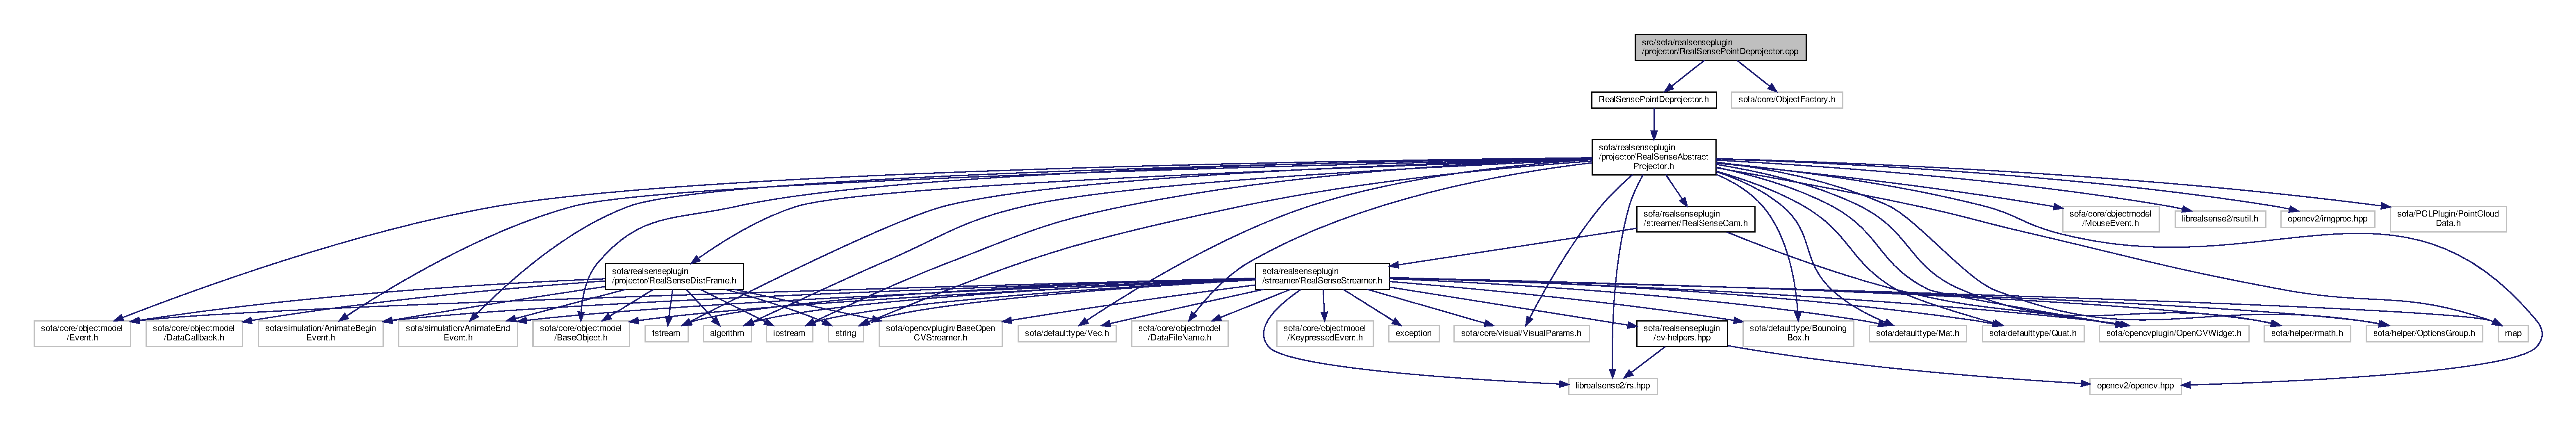
\includegraphics[width=350pt]{_real_sense_point_deprojector_8cpp__incl}
\end{center}
\end{figure}
\subsection*{Namespaces}
\begin{DoxyCompactItemize}
\item 
 \hyperlink{namespacesofa}{sofa}
\item 
 \hyperlink{namespacesofa_1_1rgbdtracking}{sofa\+::rgbdtracking}
\end{DoxyCompactItemize}
\subsection*{Variables}
\begin{DoxyCompactItemize}
\item 
int \hyperlink{namespacesofa_1_1rgbdtracking_a615e1879a9190fb07f0669c146ecc164}{sofa\+::rgbdtracking\+::\+R\+S\+Point\+Deprojector\+Class}
\end{DoxyCompactItemize}

\hypertarget{_real_sense_point_deprojector_8h}{}\section{src/sofa/realsenseplugin/projector/\+Real\+Sense\+Point\+Deprojector.h File Reference}
\label{_real_sense_point_deprojector_8h}\index{src/sofa/realsenseplugin/projector/\+Real\+Sense\+Point\+Deprojector.\+h@{src/sofa/realsenseplugin/projector/\+Real\+Sense\+Point\+Deprojector.\+h}}
{\ttfamily \#include $<$sofa/realsenseplugin/projector/\+Real\+Sense\+Abstract\+Projector.\+h$>$}\newline
Include dependency graph for Real\+Sense\+Point\+Deprojector.\+h\+:\nopagebreak
\begin{figure}[H]
\begin{center}
\leavevmode
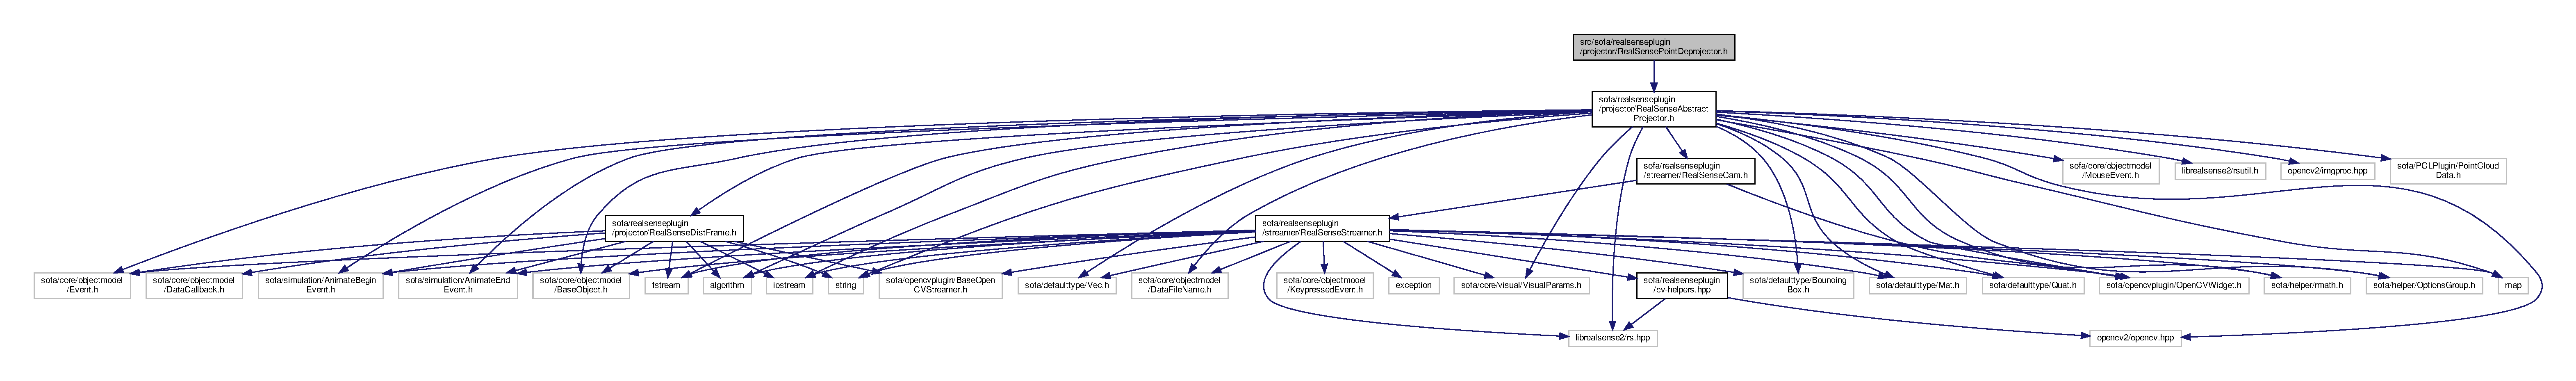
\includegraphics[width=350pt]{_real_sense_point_deprojector_8h__incl}
\end{center}
\end{figure}
This graph shows which files directly or indirectly include this file\+:\nopagebreak
\begin{figure}[H]
\begin{center}
\leavevmode
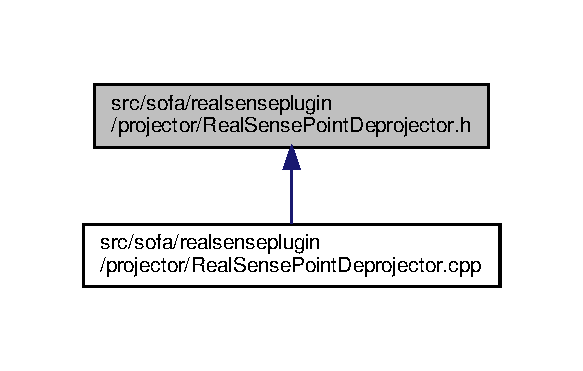
\includegraphics[width=280pt]{_real_sense_point_deprojector_8h__dep__incl}
\end{center}
\end{figure}
\subsection*{Classes}
\begin{DoxyCompactItemize}
\item 
class \hyperlink{classsofa_1_1rgbdtracking_1_1_real_sense_point_deprojector}{sofa\+::rgbdtracking\+::\+Real\+Sense\+Point\+Deprojector}
\begin{DoxyCompactList}\small\item\em The \hyperlink{classsofa_1_1rgbdtracking_1_1_real_sense_point_deprojector}{Real\+Sense\+Point\+Deprojector} class deprojects only a defined set of 2D points defined in d\+\_\+input (label input in sofa) from depth frame. \end{DoxyCompactList}\end{DoxyCompactItemize}
\subsection*{Namespaces}
\begin{DoxyCompactItemize}
\item 
 \hyperlink{namespacesofa}{sofa}
\item 
 \hyperlink{namespacesofa_1_1rgbdtracking}{sofa\+::rgbdtracking}
\end{DoxyCompactItemize}

\hypertarget{_real_sense_cam_8cpp}{}\section{src/sofa/realsenseplugin/streamer/\+Real\+Sense\+Cam.cpp File Reference}
\label{_real_sense_cam_8cpp}\index{src/sofa/realsenseplugin/streamer/\+Real\+Sense\+Cam.\+cpp@{src/sofa/realsenseplugin/streamer/\+Real\+Sense\+Cam.\+cpp}}
{\ttfamily \#include \char`\"{}Real\+Sense\+Cam.\+h\char`\"{}}\newline
{\ttfamily \#include $<$sofa/core/\+Object\+Factory.\+h$>$}\newline
Include dependency graph for Real\+Sense\+Cam.\+cpp\+:\nopagebreak
\begin{figure}[H]
\begin{center}
\leavevmode
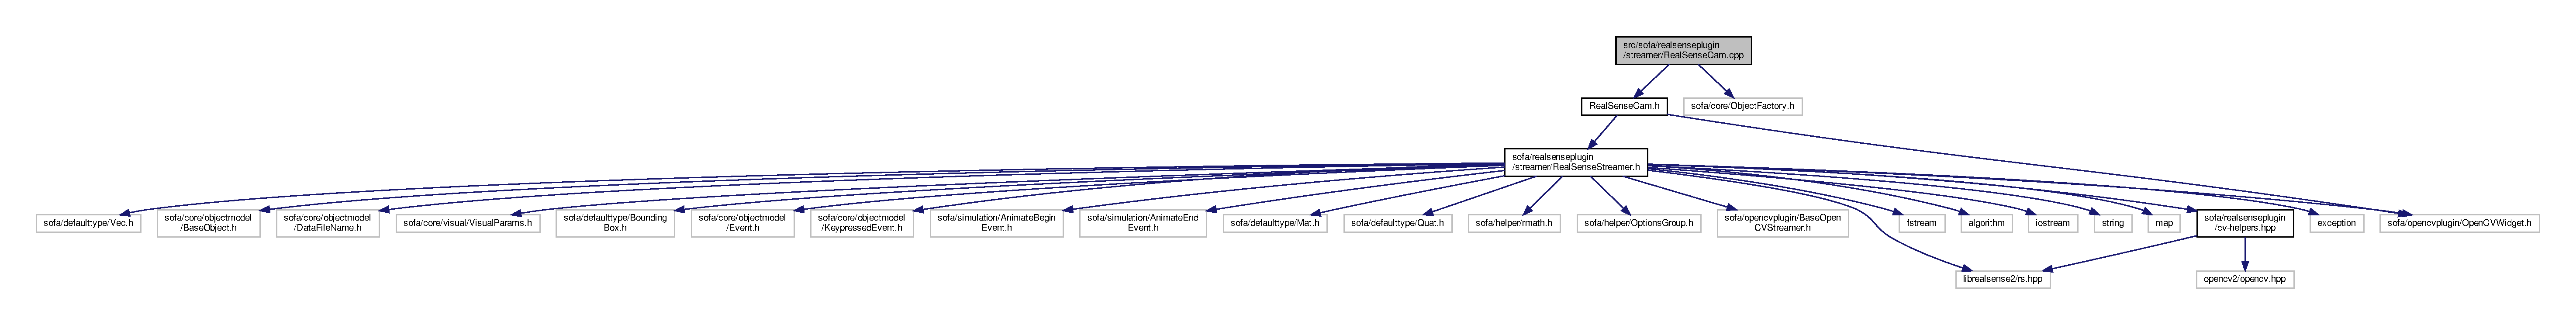
\includegraphics[width=350pt]{_real_sense_cam_8cpp__incl}
\end{center}
\end{figure}
\subsection*{Namespaces}
\begin{DoxyCompactItemize}
\item 
 \hyperlink{namespacesofa}{sofa}
\item 
 \hyperlink{namespacesofa_1_1rgbdtracking}{sofa\+::rgbdtracking}
\end{DoxyCompactItemize}
\subsection*{Variables}
\begin{DoxyCompactItemize}
\item 
int \hyperlink{namespacesofa_1_1rgbdtracking_a2430eec90f6511f570bb58f6ce29e745}{sofa\+::rgbdtracking\+::\+Real\+Sense\+Cam\+Class}
\end{DoxyCompactItemize}

\hypertarget{_real_sense_cam_8h}{}\section{src/sofa/realsenseplugin/streamer/\+Real\+Sense\+Cam.h File Reference}
\label{_real_sense_cam_8h}\index{src/sofa/realsenseplugin/streamer/\+Real\+Sense\+Cam.\+h@{src/sofa/realsenseplugin/streamer/\+Real\+Sense\+Cam.\+h}}
{\ttfamily \#include $<$sofa/realsenseplugin/streamer/\+Real\+Sense\+Streamer.\+h$>$}\newline
{\ttfamily \#include $<$sofa/opencvplugin/\+Open\+C\+V\+Widget.\+h$>$}\newline
Include dependency graph for Real\+Sense\+Cam.\+h\+:\nopagebreak
\begin{figure}[H]
\begin{center}
\leavevmode
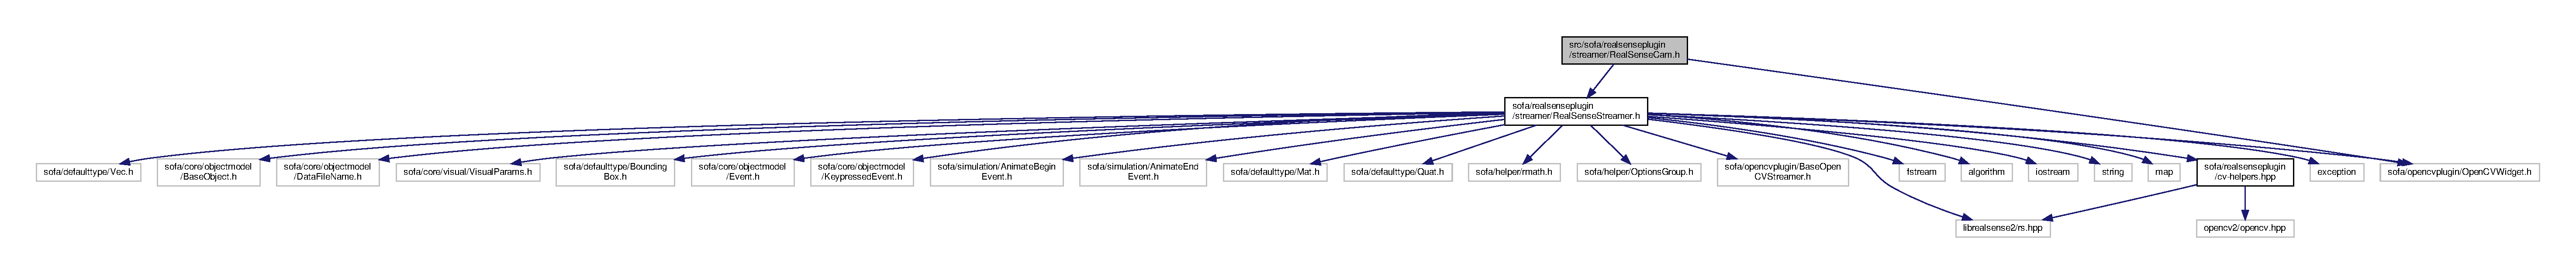
\includegraphics[width=350pt]{_real_sense_cam_8h__incl}
\end{center}
\end{figure}
This graph shows which files directly or indirectly include this file\+:\nopagebreak
\begin{figure}[H]
\begin{center}
\leavevmode
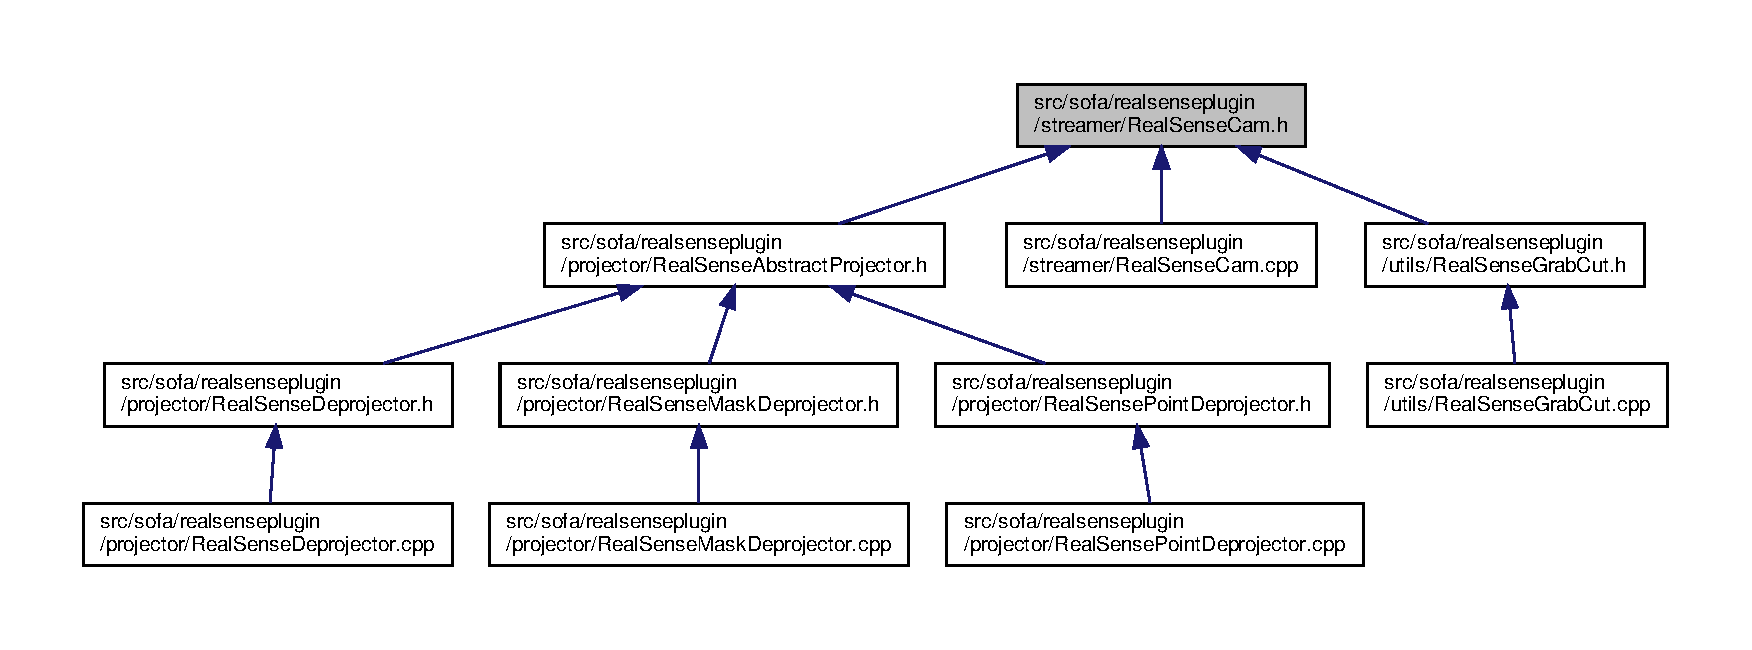
\includegraphics[width=350pt]{_real_sense_cam_8h__dep__incl}
\end{center}
\end{figure}
\subsection*{Classes}
\begin{DoxyCompactItemize}
\item 
class \hyperlink{classsofa_1_1rgbdtracking_1_1_real_sense_cam}{sofa\+::rgbdtracking\+::\+Real\+Sense\+Cam}
\begin{DoxyCompactList}\small\item\em The \hyperlink{classsofa_1_1rgbdtracking_1_1_real_sense_cam}{Real\+Sense\+Cam} class Streamer to use when only one realsense is connected. \end{DoxyCompactList}\end{DoxyCompactItemize}
\subsection*{Namespaces}
\begin{DoxyCompactItemize}
\item 
 \hyperlink{namespacesofa}{sofa}
\item 
 \hyperlink{namespacesofa_1_1rgbdtracking}{sofa\+::rgbdtracking}
\end{DoxyCompactItemize}

\hypertarget{_real_sense_multi_cam_8cpp}{}\section{src/sofa/realsenseplugin/streamer/\+Real\+Sense\+Multi\+Cam.cpp File Reference}
\label{_real_sense_multi_cam_8cpp}\index{src/sofa/realsenseplugin/streamer/\+Real\+Sense\+Multi\+Cam.\+cpp@{src/sofa/realsenseplugin/streamer/\+Real\+Sense\+Multi\+Cam.\+cpp}}
{\ttfamily \#include \char`\"{}Real\+Sense\+Multi\+Cam.\+h\char`\"{}}\newline
{\ttfamily \#include $<$sofa/core/\+Object\+Factory.\+h$>$}\newline
Include dependency graph for Real\+Sense\+Multi\+Cam.\+cpp\+:\nopagebreak
\begin{figure}[H]
\begin{center}
\leavevmode
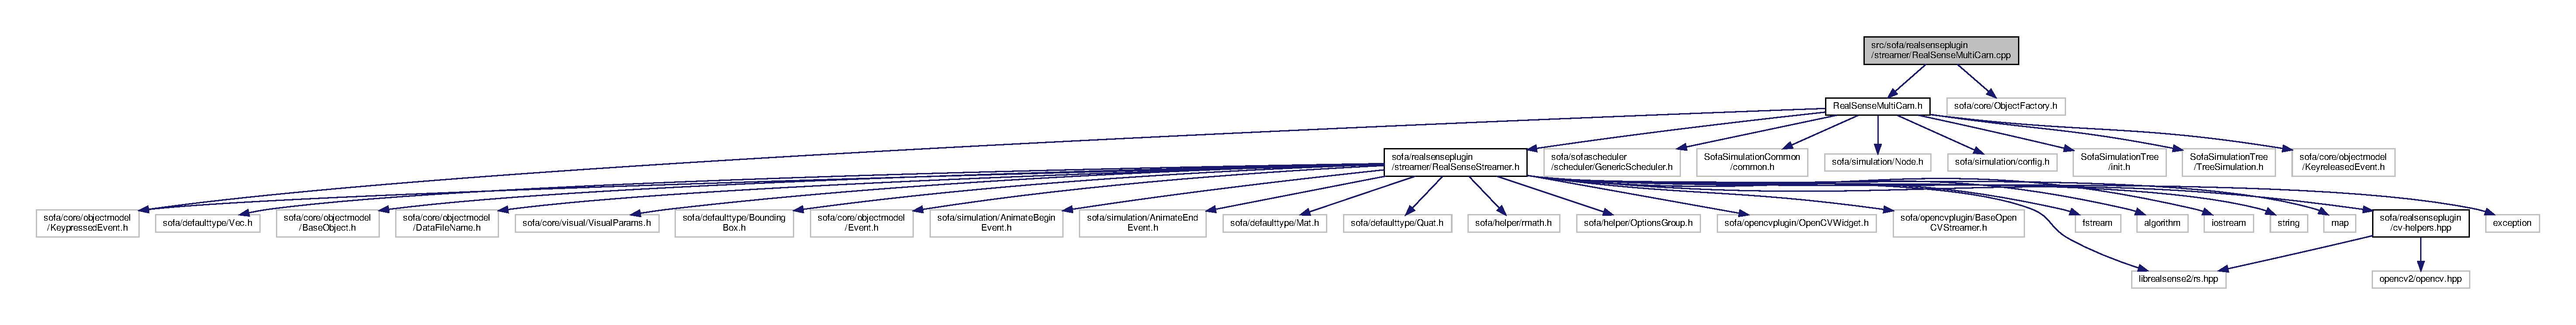
\includegraphics[width=350pt]{_real_sense_multi_cam_8cpp__incl}
\end{center}
\end{figure}
\subsection*{Namespaces}
\begin{DoxyCompactItemize}
\item 
 \hyperlink{namespacesofa}{sofa}
\item 
 \hyperlink{namespacesofa_1_1rgbdtracking}{sofa\+::rgbdtracking}
\end{DoxyCompactItemize}
\subsection*{Variables}
\begin{DoxyCompactItemize}
\item 
int \hyperlink{namespacesofa_1_1rgbdtracking_a30f0b3b59f71c94fac5ceebea2f6cf4b}{sofa\+::rgbdtracking\+::\+Real\+Sense\+Virtual\+Cam\+Class}
\item 
int \hyperlink{namespacesofa_1_1rgbdtracking_a5f7b935ae843053a8c1c4aec898c37fb}{sofa\+::rgbdtracking\+::\+Real\+Sense\+Multi\+Cam\+Class}
\end{DoxyCompactItemize}

\hypertarget{_real_sense_multi_cam_8h}{}\section{src/sofa/realsenseplugin/streamer/\+Real\+Sense\+Multi\+Cam.h File Reference}
\label{_real_sense_multi_cam_8h}\index{src/sofa/realsenseplugin/streamer/\+Real\+Sense\+Multi\+Cam.\+h@{src/sofa/realsenseplugin/streamer/\+Real\+Sense\+Multi\+Cam.\+h}}
{\ttfamily \#include $<$sofa/realsenseplugin/streamer/\+Real\+Sense\+Streamer.\+h$>$}\newline
{\ttfamily \#include $<$sofa/sofascheduler/scheduler/\+Generic\+Scheduler.\+h$>$}\newline
{\ttfamily \#include $<$Sofa\+Simulation\+Common/common.\+h$>$}\newline
{\ttfamily \#include $<$sofa/simulation/\+Node.\+h$>$}\newline
{\ttfamily \#include $<$sofa/simulation/config.\+h$>$}\newline
{\ttfamily \#include $<$Sofa\+Simulation\+Tree/init.\+h$>$}\newline
{\ttfamily \#include $<$Sofa\+Simulation\+Tree/\+Tree\+Simulation.\+h$>$}\newline
{\ttfamily \#include $<$sofa/core/objectmodel/\+Keypressed\+Event.\+h$>$}\newline
{\ttfamily \#include $<$sofa/core/objectmodel/\+Keyreleased\+Event.\+h$>$}\newline
Include dependency graph for Real\+Sense\+Multi\+Cam.\+h\+:\nopagebreak
\begin{figure}[H]
\begin{center}
\leavevmode
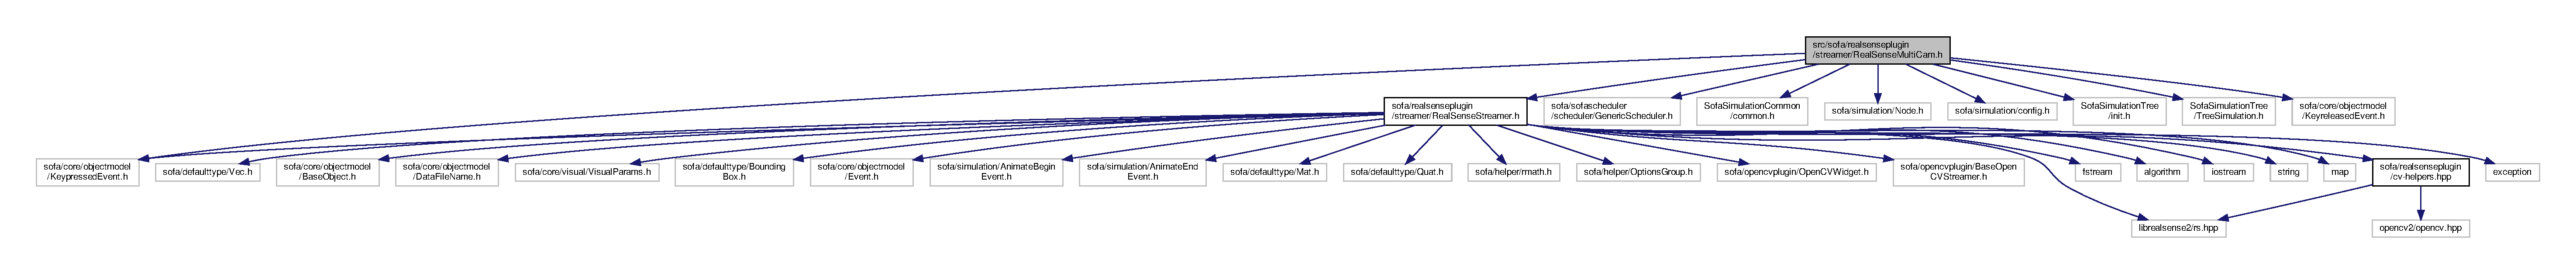
\includegraphics[width=350pt]{_real_sense_multi_cam_8h__incl}
\end{center}
\end{figure}
This graph shows which files directly or indirectly include this file\+:\nopagebreak
\begin{figure}[H]
\begin{center}
\leavevmode
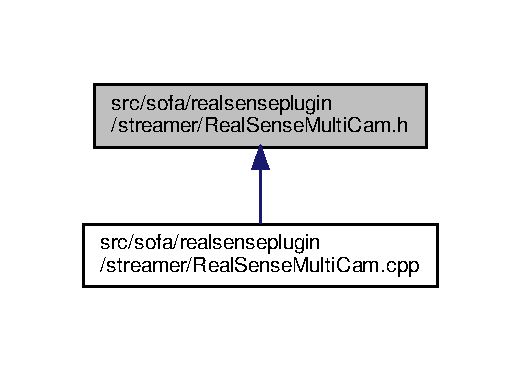
\includegraphics[width=250pt]{_real_sense_multi_cam_8h__dep__incl}
\end{center}
\end{figure}
\subsection*{Classes}
\begin{DoxyCompactItemize}
\item 
class \hyperlink{classsofa_1_1rgbdtracking_1_1_real_sense_virtual_cam}{sofa\+::rgbdtracking\+::\+Real\+Sense\+Virtual\+Cam}
\begin{DoxyCompactList}\small\item\em The \hyperlink{classsofa_1_1rgbdtracking_1_1_real_sense_virtual_cam}{Real\+Sense\+Virtual\+Cam} class virtual cam instanciated from multicam component. \end{DoxyCompactList}\item 
class \hyperlink{classsofa_1_1rgbdtracking_1_1_real_sense_multi_cam}{sofa\+::rgbdtracking\+::\+Real\+Sense\+Multi\+Cam}
\begin{DoxyCompactList}\small\item\em The \hyperlink{classsofa_1_1rgbdtracking_1_1_real_sense_multi_cam}{Real\+Sense\+Multi\+Cam} class tries listing all realsense cameras connected and instanciates Virtual\+Camera components accordingly. \end{DoxyCompactList}\end{DoxyCompactItemize}
\subsection*{Namespaces}
\begin{DoxyCompactItemize}
\item 
 \hyperlink{namespacesofa}{sofa}
\item 
 \hyperlink{namespacesofa_1_1rgbdtracking}{sofa\+::rgbdtracking}
\end{DoxyCompactItemize}

\hypertarget{_real_sense_streamer_8cpp}{}\section{src/sofa/realsenseplugin/streamer/\+Real\+Sense\+Streamer.cpp File Reference}
\label{_real_sense_streamer_8cpp}\index{src/sofa/realsenseplugin/streamer/\+Real\+Sense\+Streamer.\+cpp@{src/sofa/realsenseplugin/streamer/\+Real\+Sense\+Streamer.\+cpp}}
{\ttfamily \#include $<$sofa/realsenseplugin/streamer/\+Real\+Sense\+Streamer.\+h$>$}\newline
{\ttfamily \#include $<$sofa/core/\+Object\+Factory.\+h$>$}\newline
Include dependency graph for Real\+Sense\+Streamer.\+cpp\+:\nopagebreak
\begin{figure}[H]
\begin{center}
\leavevmode
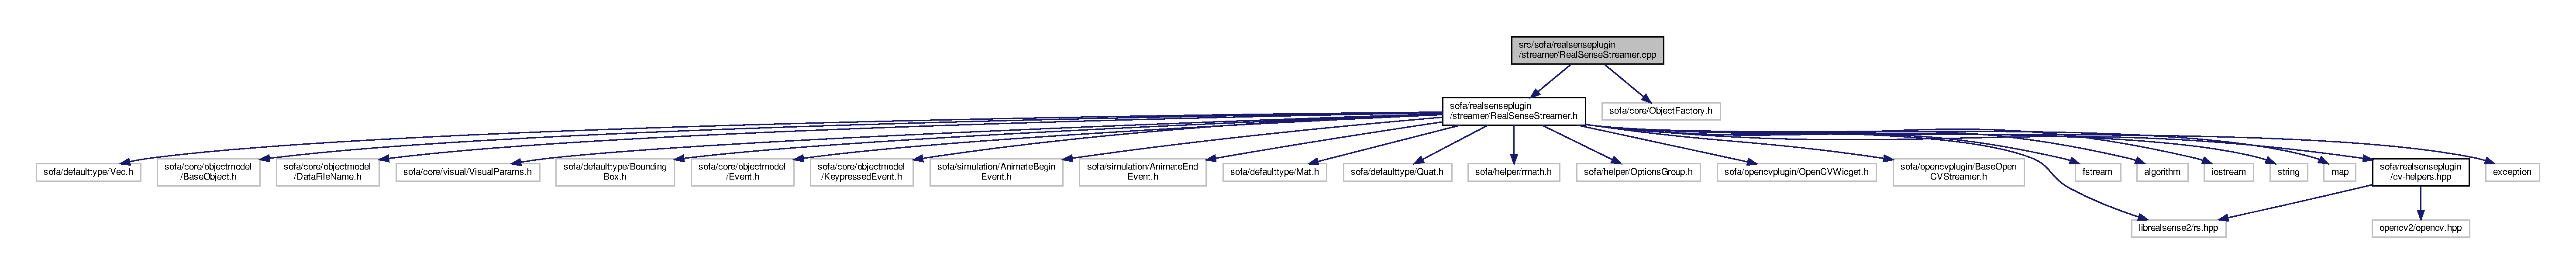
\includegraphics[width=350pt]{_real_sense_streamer_8cpp__incl}
\end{center}
\end{figure}
\subsection*{Namespaces}
\begin{DoxyCompactItemize}
\item 
 \hyperlink{namespacesofa}{sofa}
\item 
 \hyperlink{namespacesofa_1_1rgbdtracking}{sofa\+::rgbdtracking}
\end{DoxyCompactItemize}

\hypertarget{_real_sense_streamer_8h}{}\section{src/sofa/realsenseplugin/streamer/\+Real\+Sense\+Streamer.h File Reference}
\label{_real_sense_streamer_8h}\index{src/sofa/realsenseplugin/streamer/\+Real\+Sense\+Streamer.\+h@{src/sofa/realsenseplugin/streamer/\+Real\+Sense\+Streamer.\+h}}
{\ttfamily \#include $<$sofa/defaulttype/\+Vec.\+h$>$}\newline
{\ttfamily \#include $<$sofa/core/objectmodel/\+Base\+Object.\+h$>$}\newline
{\ttfamily \#include $<$sofa/core/objectmodel/\+Data\+File\+Name.\+h$>$}\newline
{\ttfamily \#include $<$sofa/core/visual/\+Visual\+Params.\+h$>$}\newline
{\ttfamily \#include $<$sofa/defaulttype/\+Bounding\+Box.\+h$>$}\newline
{\ttfamily \#include $<$sofa/core/objectmodel/\+Event.\+h$>$}\newline
{\ttfamily \#include $<$sofa/core/objectmodel/\+Keypressed\+Event.\+h$>$}\newline
{\ttfamily \#include $<$sofa/simulation/\+Animate\+Begin\+Event.\+h$>$}\newline
{\ttfamily \#include $<$sofa/simulation/\+Animate\+End\+Event.\+h$>$}\newline
{\ttfamily \#include $<$sofa/defaulttype/\+Mat.\+h$>$}\newline
{\ttfamily \#include $<$sofa/defaulttype/\+Quat.\+h$>$}\newline
{\ttfamily \#include $<$sofa/helper/rmath.\+h$>$}\newline
{\ttfamily \#include $<$sofa/helper/\+Options\+Group.\+h$>$}\newline
{\ttfamily \#include $<$sofa/opencvplugin/\+Open\+C\+V\+Widget.\+h$>$}\newline
{\ttfamily \#include $<$sofa/opencvplugin/\+Base\+Open\+C\+V\+Streamer.\+h$>$}\newline
{\ttfamily \#include $<$librealsense2/rs.\+hpp$>$}\newline
{\ttfamily \#include $<$fstream$>$}\newline
{\ttfamily \#include $<$algorithm$>$}\newline
{\ttfamily \#include $<$iostream$>$}\newline
{\ttfamily \#include $<$string$>$}\newline
{\ttfamily \#include $<$map$>$}\newline
{\ttfamily \#include $<$sofa/realsenseplugin/cv-\/helpers.\+hpp$>$}\newline
{\ttfamily \#include $<$exception$>$}\newline
Include dependency graph for Real\+Sense\+Streamer.\+h\+:\nopagebreak
\begin{figure}[H]
\begin{center}
\leavevmode
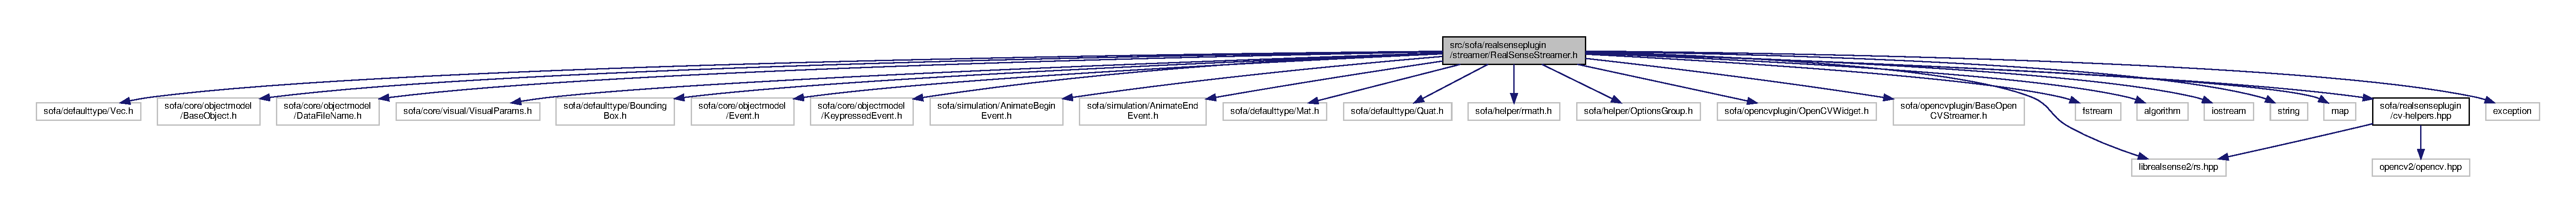
\includegraphics[width=350pt]{_real_sense_streamer_8h__incl}
\end{center}
\end{figure}
This graph shows which files directly or indirectly include this file\+:\nopagebreak
\begin{figure}[H]
\begin{center}
\leavevmode
\includegraphics[width=350pt]{_real_sense_streamer_8h__dep__incl}
\end{center}
\end{figure}
\subsection*{Classes}
\begin{DoxyCompactItemize}
\item 
class \hyperlink{classsofa_1_1rgbdtracking_1_1_real_sense_streamer}{sofa\+::rgbdtracking\+::\+Real\+Sense\+Streamer}
\begin{DoxyCompactList}\small\item\em The \hyperlink{classsofa_1_1rgbdtracking_1_1_real_sense_streamer}{Real\+Sense\+Streamer} class Abstract streamer used as a superclass for realsensecam and realsense virtual cam (used with multicam) \end{DoxyCompactList}\end{DoxyCompactItemize}
\subsection*{Namespaces}
\begin{DoxyCompactItemize}
\item 
 \hyperlink{namespacesofa}{sofa}
\item 
 \hyperlink{namespacesofa_1_1rgbdtracking}{sofa\+::rgbdtracking}
\end{DoxyCompactItemize}

\hypertarget{_real_sense_calibrator_8cpp}{}\section{src/sofa/realsenseplugin/utils/\+Real\+Sense\+Calibrator.cpp File Reference}
\label{_real_sense_calibrator_8cpp}\index{src/sofa/realsenseplugin/utils/\+Real\+Sense\+Calibrator.\+cpp@{src/sofa/realsenseplugin/utils/\+Real\+Sense\+Calibrator.\+cpp}}
{\ttfamily \#include \char`\"{}Real\+Sense\+Calibrator.\+h\char`\"{}}\newline
{\ttfamily \#include $<$sofa/core/\+Object\+Factory.\+h$>$}\newline
Include dependency graph for Real\+Sense\+Calibrator.\+cpp\+:\nopagebreak
\begin{figure}[H]
\begin{center}
\leavevmode
\includegraphics[width=350pt]{_real_sense_calibrator_8cpp__incl}
\end{center}
\end{figure}
\subsection*{Namespaces}
\begin{DoxyCompactItemize}
\item 
 \hyperlink{namespacesofa}{sofa}
\item 
 \hyperlink{namespacesofa_1_1rgbdtracking}{sofa\+::rgbdtracking}
\end{DoxyCompactItemize}
\subsection*{Variables}
\begin{DoxyCompactItemize}
\item 
int \hyperlink{namespacesofa_1_1rgbdtracking_a5a0fbb78b29abf28ac16247f111a57f6}{sofa\+::rgbdtracking\+::\+Real\+Sense\+Calibrator\+Class}
\end{DoxyCompactItemize}

\hypertarget{_real_sense_calibrator_8h}{}\section{src/sofa/realsenseplugin/utils/\+Real\+Sense\+Calibrator.h File Reference}
\label{_real_sense_calibrator_8h}\index{src/sofa/realsenseplugin/utils/\+Real\+Sense\+Calibrator.\+h@{src/sofa/realsenseplugin/utils/\+Real\+Sense\+Calibrator.\+h}}
{\ttfamily \#include $<$sofa/defaulttype/\+Vec.\+h$>$}\newline
{\ttfamily \#include $<$sofa/core/objectmodel/\+Base\+Object.\+h$>$}\newline
{\ttfamily \#include $<$sofa/core/objectmodel/\+Data\+File\+Name.\+h$>$}\newline
{\ttfamily \#include $<$sofa/core/visual/\+Visual\+Params.\+h$>$}\newline
{\ttfamily \#include $<$sofa/defaulttype/\+Bounding\+Box.\+h$>$}\newline
{\ttfamily \#include $<$sofa/core/objectmodel/\+Event.\+h$>$}\newline
{\ttfamily \#include $<$sofa/core/objectmodel/\+Keypressed\+Event.\+h$>$}\newline
{\ttfamily \#include $<$sofa/simulation/\+Animate\+Begin\+Event.\+h$>$}\newline
{\ttfamily \#include $<$sofa/simulation/\+Animate\+End\+Event.\+h$>$}\newline
{\ttfamily \#include $<$sofa/defaulttype/\+Mat.\+h$>$}\newline
{\ttfamily \#include $<$sofa/defaulttype/\+Quat.\+h$>$}\newline
{\ttfamily \#include $<$sofa/helper/rmath.\+h$>$}\newline
{\ttfamily \#include $<$sofa/helper/\+Options\+Group.\+h$>$}\newline
{\ttfamily \#include $<$sofa/opencvplugin/\+Open\+C\+V\+Widget.\+h$>$}\newline
{\ttfamily \#include $<$sofa/opencvplugin/\+Base\+Open\+C\+V\+Streamer.\+h$>$}\newline
{\ttfamily \#include $<$librealsense2/rs.\+hpp$>$}\newline
{\ttfamily \#include $<$fstream$>$}\newline
{\ttfamily \#include $<$algorithm$>$}\newline
{\ttfamily \#include $<$iostream$>$}\newline
{\ttfamily \#include $<$string$>$}\newline
{\ttfamily \#include $<$map$>$}\newline
{\ttfamily \#include $<$sofa/realsenseplugin/cv-\/helpers.\+hpp$>$}\newline
{\ttfamily \#include $<$exception$>$}\newline
Include dependency graph for Real\+Sense\+Calibrator.\+h\+:\nopagebreak
\begin{figure}[H]
\begin{center}
\leavevmode
\includegraphics[width=350pt]{_real_sense_calibrator_8h__incl}
\end{center}
\end{figure}
This graph shows which files directly or indirectly include this file\+:\nopagebreak
\begin{figure}[H]
\begin{center}
\leavevmode
\includegraphics[width=229pt]{_real_sense_calibrator_8h__dep__incl}
\end{center}
\end{figure}
\subsection*{Classes}
\begin{DoxyCompactItemize}
\item 
class \hyperlink{classsofa_1_1rgbdtracking_1_1_real_sense_calibrator}{sofa\+::rgbdtracking\+::\+Real\+Sense\+Calibrator}
\end{DoxyCompactItemize}
\subsection*{Namespaces}
\begin{DoxyCompactItemize}
\item 
 \hyperlink{namespacesofa}{sofa}
\item 
 \hyperlink{namespacesofa_1_1rgbdtracking}{sofa\+::rgbdtracking}
\end{DoxyCompactItemize}

\hypertarget{_real_sense_grab_cut_8cpp}{}\section{src/sofa/realsenseplugin/utils/\+Real\+Sense\+Grab\+Cut.cpp File Reference}
\label{_real_sense_grab_cut_8cpp}\index{src/sofa/realsenseplugin/utils/\+Real\+Sense\+Grab\+Cut.\+cpp@{src/sofa/realsenseplugin/utils/\+Real\+Sense\+Grab\+Cut.\+cpp}}
{\ttfamily \#include \char`\"{}Real\+Sense\+Grab\+Cut.\+h\char`\"{}}\newline
{\ttfamily \#include $<$sofa/core/\+Object\+Factory.\+h$>$}\newline
Include dependency graph for Real\+Sense\+Grab\+Cut.\+cpp\+:\nopagebreak
\begin{figure}[H]
\begin{center}
\leavevmode
\includegraphics[width=350pt]{_real_sense_grab_cut_8cpp__incl}
\end{center}
\end{figure}
\subsection*{Namespaces}
\begin{DoxyCompactItemize}
\item 
 \hyperlink{namespacesofa}{sofa}
\item 
 \hyperlink{namespacesofa_1_1rgbdtracking}{sofa\+::rgbdtracking}
\end{DoxyCompactItemize}
\subsection*{Variables}
\begin{DoxyCompactItemize}
\item 
int \hyperlink{namespacesofa_1_1rgbdtracking_ac0fc03382c0bfe23d9d73d844ce7ee91}{sofa\+::rgbdtracking\+::\+Real\+Sense\+Grab\+Cut\+Class}
\end{DoxyCompactItemize}

\hypertarget{_real_sense_grab_cut_8h}{}\section{src/sofa/realsenseplugin/utils/\+Real\+Sense\+Grab\+Cut.h File Reference}
\label{_real_sense_grab_cut_8h}\index{src/sofa/realsenseplugin/utils/\+Real\+Sense\+Grab\+Cut.\+h@{src/sofa/realsenseplugin/utils/\+Real\+Sense\+Grab\+Cut.\+h}}
{\ttfamily \#include $<$sofa/defaulttype/\+Vec.\+h$>$}\newline
{\ttfamily \#include $<$sofa/core/objectmodel/\+Base\+Object.\+h$>$}\newline
{\ttfamily \#include $<$sofa/core/objectmodel/\+Data\+File\+Name.\+h$>$}\newline
{\ttfamily \#include $<$sofa/core/visual/\+Visual\+Params.\+h$>$}\newline
{\ttfamily \#include $<$sofa/defaulttype/\+Bounding\+Box.\+h$>$}\newline
{\ttfamily \#include $<$sofa/core/objectmodel/\+Event.\+h$>$}\newline
{\ttfamily \#include $<$sofa/simulation/\+Animate\+Begin\+Event.\+h$>$}\newline
{\ttfamily \#include $<$sofa/simulation/\+Animate\+End\+Event.\+h$>$}\newline
{\ttfamily \#include $<$sofa/defaulttype/\+Mat.\+h$>$}\newline
{\ttfamily \#include $<$sofa/defaulttype/\+Quat.\+h$>$}\newline
{\ttfamily \#include $<$sofa/helper/rmath.\+h$>$}\newline
{\ttfamily \#include $<$sofa/helper/\+Options\+Group.\+h$>$}\newline
{\ttfamily \#include $<$opencv2/opencv.\+hpp$>$}\newline
{\ttfamily \#include $<$opencv2/imgproc.\+hpp$>$}\newline
{\ttfamily \#include $<$librealsense2/rs.\+hpp$>$}\newline
{\ttfamily \#include $<$fstream$>$}\newline
{\ttfamily \#include $<$algorithm$>$}\newline
{\ttfamily \#include $<$iostream$>$}\newline
{\ttfamily \#include $<$string$>$}\newline
{\ttfamily \#include $<$map$>$}\newline
{\ttfamily \#include $<$sofa/opencvplugin/\+Open\+C\+V\+Widget.\+h$>$}\newline
{\ttfamily \#include $<$sofa/opencvplugin/\+Base\+Open\+C\+V\+Streamer.\+h$>$}\newline
{\ttfamily \#include $<$sofa/opencvplugin/utils/\+Open\+C\+V\+Mouse\+Events.\+h$>$}\newline
{\ttfamily \#include $<$sofa/realsenseplugin/streamer/\+Real\+Sense\+Cam.\+h$>$}\newline
{\ttfamily \#include $<$sofa/realsenseplugin/cv-\/helpers.\+hpp$>$}\newline
Include dependency graph for Real\+Sense\+Grab\+Cut.\+h\+:\nopagebreak
\begin{figure}[H]
\begin{center}
\leavevmode
\includegraphics[width=350pt]{_real_sense_grab_cut_8h__incl}
\end{center}
\end{figure}
This graph shows which files directly or indirectly include this file\+:\nopagebreak
\begin{figure}[H]
\begin{center}
\leavevmode
\includegraphics[width=224pt]{_real_sense_grab_cut_8h__dep__incl}
\end{center}
\end{figure}
\subsection*{Classes}
\begin{DoxyCompactItemize}
\item 
class \hyperlink{classsofa_1_1rgbdtracking_1_1_real_sense_grab_cut}{sofa\+::rgbdtracking\+::\+Real\+Sense\+Grab\+Cut}
\end{DoxyCompactItemize}
\subsection*{Namespaces}
\begin{DoxyCompactItemize}
\item 
 \hyperlink{namespacesofa}{sofa}
\item 
 \hyperlink{namespacesofa_1_1rgbdtracking}{sofa\+::rgbdtracking}
\end{DoxyCompactItemize}
\subsection*{Macros}
\begin{DoxyCompactItemize}
\item 
\#define \hyperlink{_real_sense_grab_cut_8h_a6f89e724bdd5e5bfc46f749348191dbb}{E\+R\+O\+S\+I\+O\+N\+\_\+\+K\+E\+R\+N\+E\+L\+\_\+\+S\+I\+ZE}~cv\+::\+Size(3, 3)
\end{DoxyCompactItemize}


\subsection{Macro Definition Documentation}
\mbox{\Hypertarget{_real_sense_grab_cut_8h_a6f89e724bdd5e5bfc46f749348191dbb}\label{_real_sense_grab_cut_8h_a6f89e724bdd5e5bfc46f749348191dbb}} 
\index{Real\+Sense\+Grab\+Cut.\+h@{Real\+Sense\+Grab\+Cut.\+h}!E\+R\+O\+S\+I\+O\+N\+\_\+\+K\+E\+R\+N\+E\+L\+\_\+\+S\+I\+ZE@{E\+R\+O\+S\+I\+O\+N\+\_\+\+K\+E\+R\+N\+E\+L\+\_\+\+S\+I\+ZE}}
\index{E\+R\+O\+S\+I\+O\+N\+\_\+\+K\+E\+R\+N\+E\+L\+\_\+\+S\+I\+ZE@{E\+R\+O\+S\+I\+O\+N\+\_\+\+K\+E\+R\+N\+E\+L\+\_\+\+S\+I\+ZE}!Real\+Sense\+Grab\+Cut.\+h@{Real\+Sense\+Grab\+Cut.\+h}}
\subsubsection{\texorpdfstring{E\+R\+O\+S\+I\+O\+N\+\_\+\+K\+E\+R\+N\+E\+L\+\_\+\+S\+I\+ZE}{EROSION\_KERNEL\_SIZE}}
{\footnotesize\ttfamily \#define E\+R\+O\+S\+I\+O\+N\+\_\+\+K\+E\+R\+N\+E\+L\+\_\+\+S\+I\+ZE~cv\+::\+Size(3, 3)}


%--- End generated contents ---

% Index
\backmatter
\newpage
\phantomsection
\clearemptydoublepage
\addcontentsline{toc}{chapter}{Index}
\printindex

\end{document}
